%%
%% This is file `ubcsample.tex',
%% generated with the docstrip utility.
%
% The original source files were:
%
% ubcthesis.dtx  (with options: `ubcsampletex')
%% 
%% This file was generated from the ubcthesis package.
%% --------------------------------------------------------------
%% 
%% Copyright (C) 2001
%% Michael McNeil Forbes
%% mforbes@alum.mit.edu
%% 
%% This file may be distributed and/or modified under the
%% conditions of the LaTeX Project Public License, either version 1.2
%% of this license or (at your option) any later version.
%% The latest version of this license is in
%%    http://www.latex-project.org/lppl.txt
%% and version 1.2 or later is part of all distributions of LaTeX
%% version 1999/12/01 or later.
%% 
%% This program is distributed in the hope that it will be useful,
%% but WITHOUT ANY WARRANTY; without even the implied warranty of
%% MERCHANTABILITY or FITNESS FOR A PARTICULAR PURPOSE.  See the
%% LaTeX Project Public License for more details.
%% 
%% This program consists of the files ubcthesis.dtx, ubcthesis.ins, and
%% the sample figures fig.eps and fig.fig.
%% 
%% This file may be modified and used as a base for your thesis without
%% including the licence agreement as long as the content (i.e. textual
%% body) of the file is completely rewritten. You must, however, change
%% the name of the file.
%% 
%% This file may only be distributed together with a copy of this
%% program. You may, however, distribute this program without generated
%% files such as this one.
%% 

% This Sample thesis requires \LaTeX2e
\NeedsTeXFormat{LaTeX2e}[1995/12/01]
\ProvidesFile{ubcsample.tex}[2015/05/31 v1.72 ^^J
 University of British Columbia Sample Thesis]
% This is the \documentclass[]{} command.  The manditory argument
% specifies the "flavour" of thesis (ubcthesis for UBC).  The
% optional arguments (in []) specify options that affect how the
% thesis is displayed.  Please see the ubcthesis documentation for
% details about the options.
\documentclass[msc,twoside,final]{ubcthesis}
%
% To compile this sample thesis, issue the following commands:
% latex ubcsample
% bibtex ubcsample
% latex ubcsample
% latex ubcsample
% latex ubcsample
%
% To view use xdvi (on unix systems):
% xdvi ubcsample.dvi
%
% To make a postscript file, use dvips:
% dvips -o ubcsample.ps ubcsample.dvi
%
% To view the postscript file, use ghostview or gv (on unix systems):
% gv ubcsample.ps
%
%************************************************
% Optional packages.
%
% The use of these packages is optional, but they provide various
% tools for more flexible formating.  The sample thesis uses these,
% but if you remove the example code, you should be able to exclude
% these packages.  Only standard packages have been described here;
% they should be installed with any complete LaTeX installation, but
% if not, you can find them at the Comprehensive TeX Archive Network
% (CTAN): http://www.ctan.org/
%

%******** afterpage ***************************
% This package allows you to issue commands at the end of the current
% page.  A good use for this is to use the command
% \afterpage{\clearpage} right after a figure.  This will cause the
% figure to be inserted on the page following the current one (or on
% the current page if it will fit) but will not break the page in the
% middle.
\usepackage{afterpage}

%******** float *********************************
% This package allows you to customize the style of
% "floats"---floating objects such as figures and tables.  In
% addition, it allows you to define additional floating objects which
% may be included in a list similar to that produces by \listoftables
% and \listoffigures.  Common uses include introducing floats for
% programs and other code bits in Compute Science and Chemical Schema.
\usepackage{float}

%******** tocloft *******************************
% This package allows you to customize and define custom lists such
% as a list of programs or Chemical Scheme.  Note: if you use the
% subfigure package, you must specify that you do as an option here.
% The title option uses the default formatting.  We do not use this
% here as the default formatting is acceptable.  Use the float
% package instead unless you need the extra formatting control
% provided by tocloft.
%\usepackage[subfigure, titles]{tocloft}

%******** alltt *********************************
% The alltt package allows you to include files and have them
% formatted in a verbatim fashion.  This is useful for including
% source code from an additional file.
%\usepackage{alltt}

%******** listings ******************************
% The listings package may be used to include chunks of source code
% and has facilities for pretty-printing many languages.
%\usepackage{listings}

%******** longtable *****************************
% The longtable package allows you to define tables that span
% multiple pages.
\usepackage{longtable}

%******** graphics and graphicx *****************
% This allows you to include encapsulated postscript files.  If you
% don't have this, comment the \includegraphics{} line following the
% comment "%includegraphics" later in this file.
\usepackage{graphicx}

%******** subfigure *****************************
% The subfigure package allows you to include multiple figures and
% captions within a single figure environment.
%\usepackage{subfigure}

%******** here **********************************
% The here package gives you more control over the placement of
% figures and tables.  In particular, you can specify the placement
% "H" which means "Put the figure here" rather than [h] which means
% "I would suggest that you put the figure here if you think it looks
% good."
\usepackage{here}

%******** pdflscape ********************************
% This allows you to include landscape layout pages by using the
% |landscape| environment.  The use of |pdflscape| is preferred over
% the standard |lscape| package because it automatically rotates the
% page in the pdf file for easier reading.  (Thanks to Joseph Shea
% for pointing this out.)
\usepackage{pdflscape}

%******** natbib ********************************
% This is a very nice package for bibliographies.  It includes options
% for sorting and compressing bibliographic entries.
%\usepackage[numbers,sort&compress]{natbib}

%******** psfrag ******************************
% This allows you to replace text in postscript pictures with formated
% latex text.  This allows you to use math in graph labels
% etc. Uncomment the psfrag lines following the "%psfrag" comment
% later in this file if you don't have this package.  The replacements
% will only be visible in the final postscript file: they will be
% listed in the .dvi file but not performed.
\usepackage{psfrag}

%******** hyperref *****************************
% Please read the manual:
% http://www.tug.org/applications/hyperref/manual.html
%
% This adds hyperlinks to your document: with the right viewers (later
% versions of xdvi, acrobat with pdftex, latex2html etc.) this will
% make your equation, figure, citation references etc. hyperlinks so
% that you can click on them.  Also, your table of contents will be
% able to take you to the appropriate sections.  In the viewers that
% support this, the links often appear with an underscore.  This
% underscore will not appear in printed versions.
%
% Note: if you do not use the hypertex option, then the dvips driver
% may be loaded by default.  This will cause the entries in the list
% of figures and list of tables to be on a single line because dvips
% does not deal with hyperlinks on broken lines properly.
%
% NOTE: HYPERREF is sensitive to the ORDER in which it is LOADED.
% For example, it must be loaded AFTER natbib but BEFORE newly
% defined float environments.  See the README file with the hyperref
% for some help with this.  If you have some very obscure errors, try
% first disabling hyperref.  If that fixes the problem, try various
% orderings.
%
% Note also that there is a bug with versions before 2003/11/30
% v6.74m that cause the float package to not function correctly.
% Please ensure you have a current version of this package.  A
% warning will be issued if you leave the date below but do not have
% a current version installed.
%
% Some notes on options: depending on how you build your files, you
% may need to choose the appropriate option (such as [pdftex]) for the
% backend driver (see the hyperref manual for a complete list).  Also,
% the default here is to make links from the page numbers in the table
% of contents and lists of figures etc.  There are other options:
% excluding the [linktocpage] option will make the entire text a
% hyperref, but for some backends will prevent the text from wrapping
% which can look terrible.  There is a [breaklinks=true] option that
% will be set if the backend supports (dvipdfm for example supports
% it but does not work with psfrag.)
%
% Finally, there are many options for choosing the colours of the
% links.  These will be included by default in future versions but
% you should probably consider changing some now for the electronic
% version of your thesis.
\usepackage[unicode=true,
  linktocpage,
  linkbordercolor={0.5 0.5 1},
  citebordercolor={0.5 1 0.5},
  linkcolor=blue]{hyperref}
  
 % Here is what I have added
 %% Useful packages
\usepackage{amsmath}
\usepackage{graphicx}
\usepackage[colorinlistoftodos]{todonotes}
\usepackage{breqn}
\usepackage{multirow}


%%New packages
\usepackage{physics}
\usepackage{caption}
\usepackage{subcaption}


% If you would like to compile this sample thesis without the
% hyperref package, then you will need to comment out the previous
% \usepackage command and uncomment the following command which will
% put the URL's in a typewriter font but not link them.
%\newcommand\url[1]{\texttt{#1}}

%******** setspace *******************************
% The setspace package allows you to manually set the spacing of the
% file.  UBC may require 1.5 spacing for microfilming of theses.  In
% this case you may obtain this by including this package and issuing
% one of the following commands:
%\usepackage{setspace}
%\singlespacing
%\onehalfspacing
%\doublespacing
% Here is a way to turn off global indenting, but be able to indent still
\newlength\tindent
\setlength{\tindent}{\parindent}
\setlength{\parindent}{0pt}
\renewcommand{\indent}{\hspace*{\tindent}}

% These commands are optional.  The defaults are shown.  You only
% need to include them if you need a different value
\institution{The University Of British Columbia}

% If you are at the Okanagan campus, then you should specify these
% instead.
%\faculty{The College of Graduate Studies}
%\institutionaddress{Okanagan}
\faculty{The Faculty of Graduate and Postdoctoral Studies}
\institutionaddress{Vancouver}

% You can issue as many of these as you have...
\previousdegree{B.Sc., Metropolitan State University of Denver, 2016}

% You can override the option setting here.
% \degreetitle{Jack of All Trades}

% These commands are required.
\title{Non-Smooth Dynamics in the Stommel Model of the Thermohaline Circulation}
\author{Cody Griffith}
\copyrightyear{2018}
\submitdate{\monthname\ \number\year} % The "\ " is required after
                                      % \monthname to prevent the
                                      % command from eating the space.
\program{Mathematics}

% These commands are presently not required for UBC theses as the
% advisor's name and title are not presently required anywhere.
\advisor{Rachel Kuske}
\advisortitle{Professor of Mathematics}

% One might want to override the format of the section and chapter
% numbers.  This shows you how to do it.  Note that the current
% format is acceptable for submission to the FoGS: If you wish to modify
% these, you should check with the FoGS explicity. prior to making
% the modifications.
\renewcommand\thepart         {\Roman{part}}
\renewcommand\thechapter      {\arabic{chapter}}
\renewcommand\thesection      {\thechapter.\arabic{section}}
\renewcommand\thesubsection   {\thesection.\arabic{subsection}}
\renewcommand\thesubsubsection{\thesubsection.\arabic{subsubsection}}
\renewcommand\theparagraph    {\thesubsubsection.\arabic{paragraph}}
\renewcommand\thesubparagraph {\theparagraph.\arabic{subparagraph}}

\setcounter{tocdepth}{2}
\setcounter{secnumdepth}{2}
\setcounter{figure}{0}

% Here is an example of a "Program" environment defined with the
% "float" package.  The list of programs will be stored in the file
% ubcsample.lop and the numbering will start with the chapter
% number.  The style will be "ruled".
\floatstyle{ruled}
\newfloat{Program}{htbp}{lop}[chapter]

\usepackage[margin=1.25in]{geometry}

\raggedbottom


% Here is the start of the document.
\begin{document}

%% This starts numbering in Roman numerals as required for the thesis
%% style and is mandatory.
\frontmatter

%%% The order of the following components should be preserved.  The order
%%% listed here is the order currently required by FoGS:        \\
%%% Title (Mandatory)                                           \\
%%% Preface (Mandatory if any collaborator contributions)       \\
%%% Abstract (Mandatory)                                        \\
%%% List of Contents, Tables, Figures, etc. (As appropriate)    \\
%%% Acknowledgements (Optional)                                 \\
%%% Dedication (Optional)                                       \\

\maketitle 	%% Mandatory

%% Committee Page
The following individuals certify that they have read, and recommend to the Faculty of Graduate and Postdoctoral Studies for acceptance, a thesis entitled:
$$\textbf{Non-Smooth Dynamics in the Stommel Model of the Thermohaline Circulation}$$

submitted by \textbf{Cody Griffith} in partial fulfillment of the requirements of the degree of \textbf{Master of Science} in \textbf{Applied Mathematics}.\\
\\

\textbf{Examining Committee:}\\
\\
\textbf{Rachel Kuske, Professor of Mathematics}\\
Supervisor\\
\\
\textbf{Brian Wetton, Professor of Mathematics}\\
Supervisory Committee Member

\begin{abstract}                %% Mandatory -  maximum 350 words
We analyzed the non-smooth dynamics for the Stommel model for thermohaline circulation with additional mechanisms like slowly varying bifurcation parameters and high frequency oscillatory forcing. Our goal was to find an analytic approximation to the tipping point and forced bifurcation induced by the new features in the model. We first analyze a simpler one component model that has similar structure to the Stommel model and gradually build in more complexity into the one component problem and study the effects on the tipping point. In this context, we compare the relative strengths of the non-smooth effects on the tipping point to the smooth effects which has been previously studied. With the one component model understood, we then apply similar methods to the Stommel model and study the effects on the non-smooth tipping points and forced bifurcations. With these results we have the ability to fully describe the hysteresis found in the Stommel model.
\end{abstract}

\chapter{Lay Summary}
We study the behavior of the thermohaline circulation. This circulation is responsible for moving water from around the globe and thus a model was created to understand how it functions. Work has previously been done on certain components of this model, but the analysis we provide is done around the less studied pieces known as the non-smooth dynamics. We ultimately provide a solution to the non-smooth dynamics and even incorporate more mechanisms in the original model to account for a larger class of observable behavior. This allows for a better understanding of the thermohaline circulation and could help predict and prepare for sudden abrupt changes to the ocean currents that drive our climate.

\chapter{Preface} % Manditory if any of the conditions are met
This thesis is original, unpublished, independent work by the author, C. Griffith.

% Table of contents
\tableofcontents

\listoffigures

\newpage

\chapter{Acknowledgments}
I would like to thank my supervisor Rachel Kuske for the project idea and guidance as well as my committee member Brian Wetton for helping me professionally through graduate school.
\newline

Special thanks are given to my peers Tim Jaschek and Matthias Kl{\"o}ckner for their aide in writing and support throughout the entire degree. Couldn't have done it without you both!

\newpage

%%%%% My Work
\mainmatter
\chapter{Introduction}
\label{chap:introduction}
The main focus of studying dynamical systems is to understand the possible states an observable solution can experience and with most engineering, physics or even chemical systems, this is a cumbersome task. Often we find parameters inherent in the model for the system to play huge roles in the dynamical behavior and can be the difference between a system being capable of finding an equilibrium or not. When we find a parameter that has this effect, we call it a bifurcation parameter as there is some value that can be found that suddenly bifurcates the behavior of the system. The canonical example and one of the first to be studied was the system that contained a saddle-node bifurcation

\begin{equation}\label{eq:intro_saddlenode}
\dot{x}=a-x^2.
\end{equation}

\begin{figure}[H]
\centering
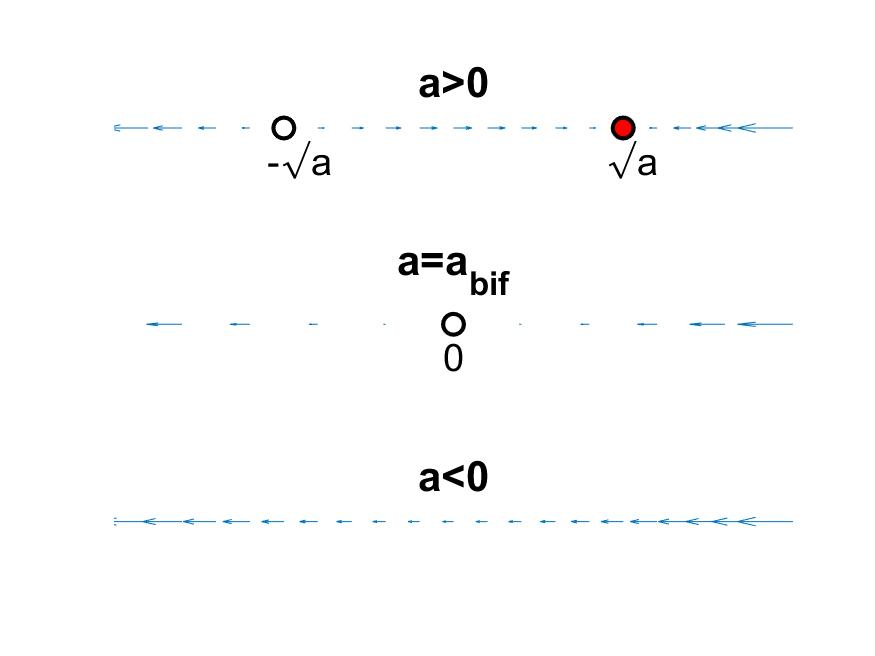
\includegraphics[width=\linewidth]{intro/saddlenode.jpg}
\caption{Vector field of a saddle-node bifurcation}
\label{fig:intro_saddlenode}
\end{figure}


\begin{figure}[H]
\centering
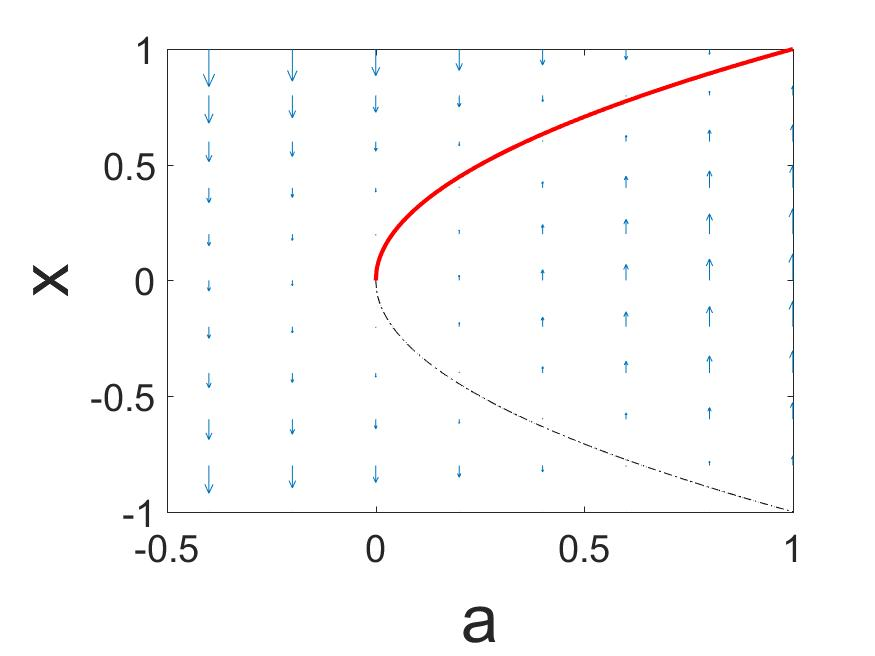
\includegraphics[width=.7\linewidth]{intro/saddlenode_bif_diagram.jpg}
\caption{Diagram of saddle-node bifurcation}
\label{fig:intro_saddlenode_bif_diagram}
\end{figure}



In figure~\ref{fig:intro_saddlenode} we show the vector field of the system that contains a saddle-node bifurcation. The equilibrium of this system is $x=\pm \sqrt{a}$ for any $a>0$ where stable equilibrium points with solid lines and unstable with dash-dotted lines. Notice that at $a=0$ and when $a<0$ we are no longer unable to find a stable equilibrium. This is known to be the simplest example of different qualitative behavior arising from a change in the parameter and it happens by two equilibria annihilating. In figure~\ref{fig:intro_saddlenode_bif_diagram} we plot the same system against the parameter $a$, which we call the phase plane. Here we still see the region with two equilibrium, the bifurcation and the region of no stability. Although, there are many types of bifurcations that have arisen in different systems that each have their own key properties. Studying these properties lead to a deeper understanding of the system on both the global and local scale. Much work has been done on systems that have smooth bifurcations due to the analysis being easier to perform, but non-smooth dynamics still are present in the physical world.

Non-smooth bifurcations are a topic that arise in special systems and for how frequent they appear, they have not been studied nearly as much as their smooth counter parts. This paper discusses the role of the non-smooth saddle-node bifurcation in a simplified one-dimensional system in \autoref{chap:oneD} as well as in the classic two-dimensional Stommel model for Thermohalcine current dynamics in \autoref{chap:twoD}. But many interesting ocean and weather mechanisms may be incorporated into the Stommel model to provide more realistic predictions for weather patterns. We choose to study slowly varying bifurcation parameters and their effect on the stability of a system while contrasting this with non-autonomous oscillatory forcing. The interaction of these features create complex dynamics around the standard bifurcations and can lead to early bifurcation or delayed tipping. For the one-dimensional system, a detailed analysis of these features is done on the smooth bifurcation by Zhu \& Kuske \cite{zhu2015tipping}.

\section*{Stommel Model}

Global circulation models have primarily focused on three different categories: 
\begin{itemize}
\item Atmospheric- the effect of greenhouse gases have on the atmosphere,
\item Oceanic- the effect of tides and interaction of temperature with salinity in the ocean,
\item Sea ice and land surface components.
\end{itemize}
These categories all contribute significantly to the overall prediction of weather and climate for the planet, which has importance to just about every industry and economy. Failure to adhere to and prepare for sudden changes in the climate led to drastic situations like severe droughts or ocean acidification. Atmospheric models have been vastly studied but far less work has been done on the contribution from the ocean and the dynamics that drive the tides and current.

A key feature of oceanic contributions is when patterns form around regions of bi-stability of temperature and salinity. An example of this is the thermohaline circulation (THC) which experience abrupt qualitative changes at certain points, see Alley \cite{alley2003abrupt},
Marotzke \cite{marotzke2000abrupt},
or Rahmstorf \cite{rahmstorf2000thermohaline} and
\cite{rahmstorf2002ocean}. Just earlier this year Rahmstorf was able to find evidence of weakening occurring around these abrupt changes in a system of ocean patterns known as the Atlantic meridional overturning circulation (AMOC) \cite{caesar2018AMOC}. This is the first evidence of ocean dynamics responding to temperature change on the surface and can help further predict the future of the system. It is imperative that appropriate action is taken to prepare for the future of these type of systems as they are outside our realm of control. 

To study these phenomenon we create parametric models to replicate the dynamics we observe. Initially, Henry Stommel proposed the two box model in 1961 to understand the physics of the THC, shown in figure~\ref{fig:stommel_boxes}. In Stommel \cite{stommel1961thermohaline}, it is suggested that there are actually two different stability regimes which even overlap in the system that is proposed and concluded that oceanic dynamics behave very similarly about these equilibria. These type of systems have since been a heavily studied area for both climatology due to the wide ranging applications and dynamical systems for its generalization into dual stability.

\begin{figure}[H]
\centering
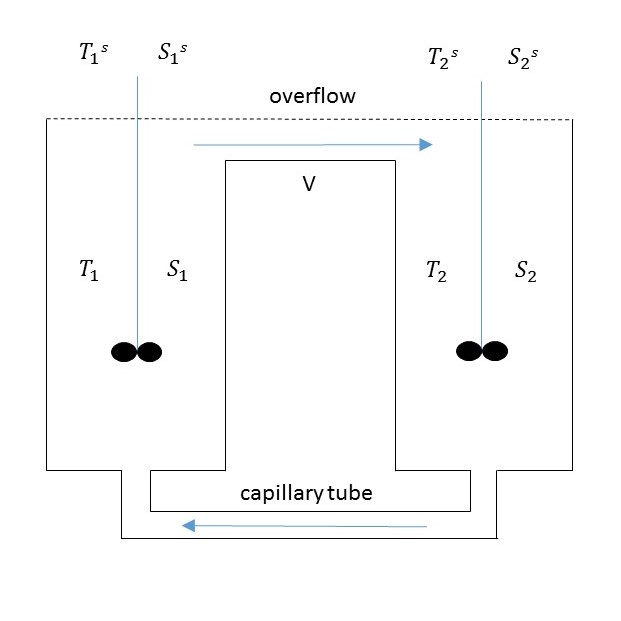
\includegraphics[width=0.7\textwidth]{intro/box.jpg}
\caption{The Stommel Two Box Model: Differing volume boxes with a temperature and salinity, $T_i$ and $S_i$. The boxes are connected by an overflow and capillary tube that has a flow $V$. There is also a surface temperature and salinity for each box, ${T_i}^s$ and ${S_i}^s$. We assume that there is some stirring to give a well mixed structure.}
\label{fig:stommel_boxes}
\end{figure}

With emphasis on mathematics, the focus of this paper is on developing an effective approach to problems with bi-stability and additional mechanisms and thus the physical quantities are brushed aside in favor of their non-dimensional alternatives. The non-dimensionalized Stommel Model is represented with the system

\begin{equation}
  \begin{aligned}
   \dot{T} & =  \eta_1-T(1+|T-S|), \\
   \dot{S}     & =  \eta_2-S(\eta_3+|T-S|). 
  \end{aligned}
\end{equation}

The variables $T$ and $S$ are the temperature and salinity respectively, the parameters $\eta_1$, $\eta_2$, and $\eta_3$ are all dimensionless quantities that all have physical interpretation to the relaxation times and volumes of the box. Where $\eta_1$ is thought of as the thermal variation, $\eta_2$ as the saline variation otherwise known as the freshwater flux, and $\eta_3$ as the ratio of relaxation times of temperature and salinity. Here $\eta_1$ is a positive quantity that takes any value whereas $\eta_3$ is also positive but has the property to determine the orientation of the equilibria. A standard orientation will be when $\eta_3<1$, $\eta_3=1$ is a special case and $\eta_3>1$ will have reverse orientation, this is seen in figure~\ref{fig:Stommel_bif_plots}. This is due to the nature of the parameter, when $\eta_3=1$, the relaxation rates for both the thermal and salinity variables are the same and hence we lose the dual stability.

The parameter $\eta_2$ is the most interesting as different values cause major qualitative and quantitative changes in the dynamics of the system. These changes have been discovered at two different points in the system, each being called either a smooth or a non-smooth saddle-node bifurcation.

It is convenient to view this system in terms of the variable $V=T-S$, which leads to the system

\begin{equation}\label{eq:basic_stommel}
  \begin{aligned}
   \dot{T} & =  \eta_1-T(1+|V|), \\
   \dot{V}     & =  (\eta_1-\eta_2)-V|V|-T+\eta_3(T-V).
  \end{aligned}
\end{equation}

\begin{figure}[H]
\centering
\begin{subfigure}{.5\textwidth}
  \centering
  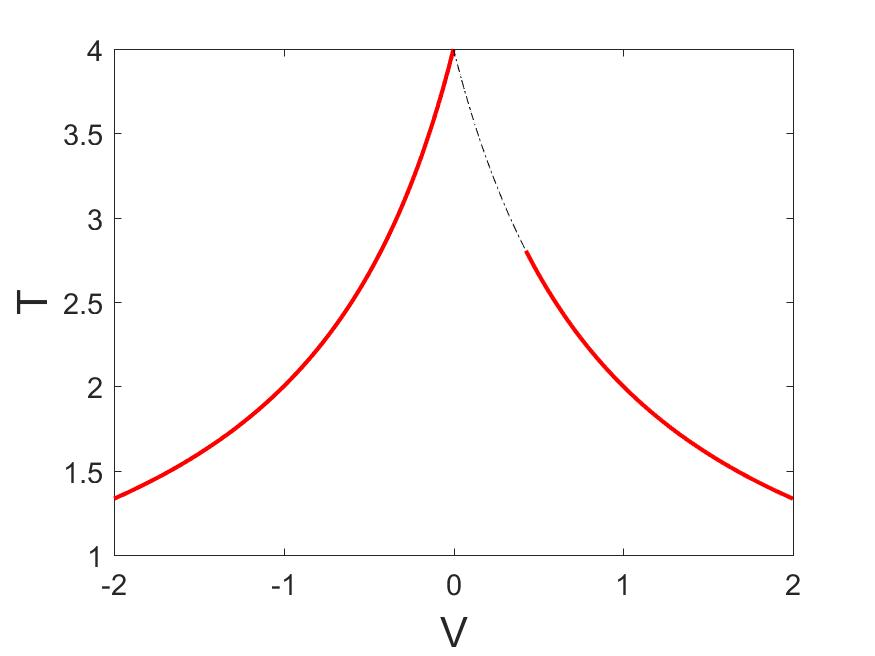
\includegraphics[width=\linewidth]{intro/T_equil.jpg}
  \caption{$V$ vs. $T$}
  \label{fig:Tequil}
\end{subfigure}%
\begin{subfigure}{.5\textwidth}
  \centering
  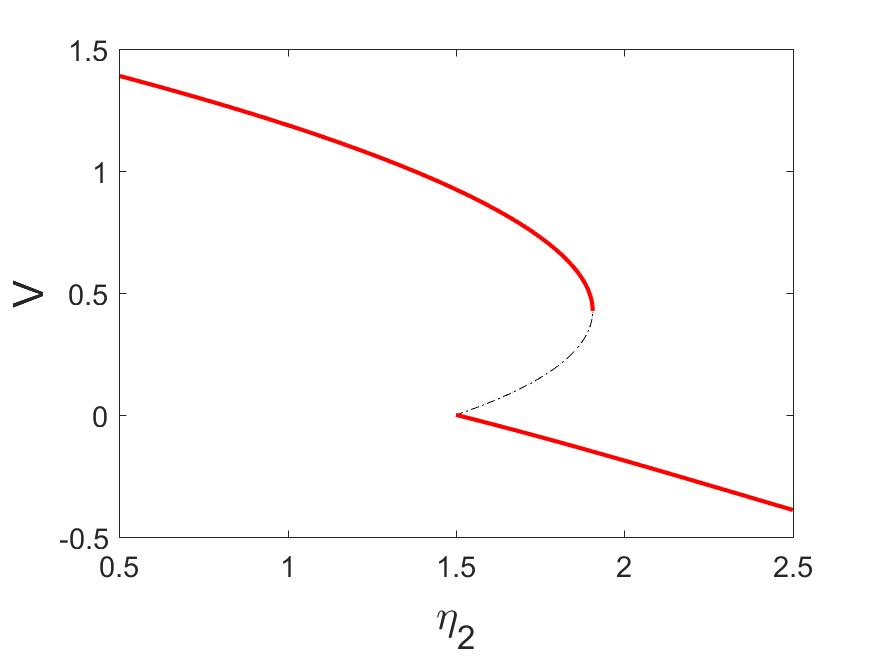
\includegraphics[width=\linewidth]{intro/V_bif.jpg}
  \caption{$\eta_2$ vs. $V$}
  \label{fig:Vbif}
\end{subfigure}
\caption{The equilibria of the non-dimensionalized system \eqref{eq:basic_stommel}. Parameters values are $\eta_1=4$ and $\eta_3=.375$. We see non-smooth behavior happening in both plots when $V=0$. The red line indicates a stable branch where the dashed dotted line is for an unstable branch.}
\label{fig:systemequil}
\end{figure}

As shown in figure~\ref{fig:systemequil}, the equilibrium curves reveal much about the dynamics. In (a) the graph of the equilibria for $V$ vs. $T$ shows non-smooth behavior occurring at $V=0$ and in (b) the two types of bifurcation appear clearly in the graph of equilibria for $\eta_2$ vs. $V$. In this plot, both the upper and lower branches of the equilibrium are stable with the middle branch being unstable. The stable branches relate to which variable is dominate. For the lower branch, we call this the halcine branch, and the upper branch the thermal branch. The location of the non-smooth bifurcation is found analytically, $({\eta_2}_{ns}V_{ns},T_{ns})=(\eta_1\eta_3,0,\eta_1)$, and the smooth bifurcation, $({\eta_2}_{\text{smooth}},V_{\text{smooth}},T_{\text{smooth}})$, is the only real solution to a cubic polynomial. The smoothness of each bifurcation is apparent and arise from the absolute value term in the defining dynamics of \eqref{eq:basic_stommel}, which is non-smooth only at $V=0$.

\begin{figure}[H]
\centering
\begin{subfigure}{.5\textwidth}
  \centering
  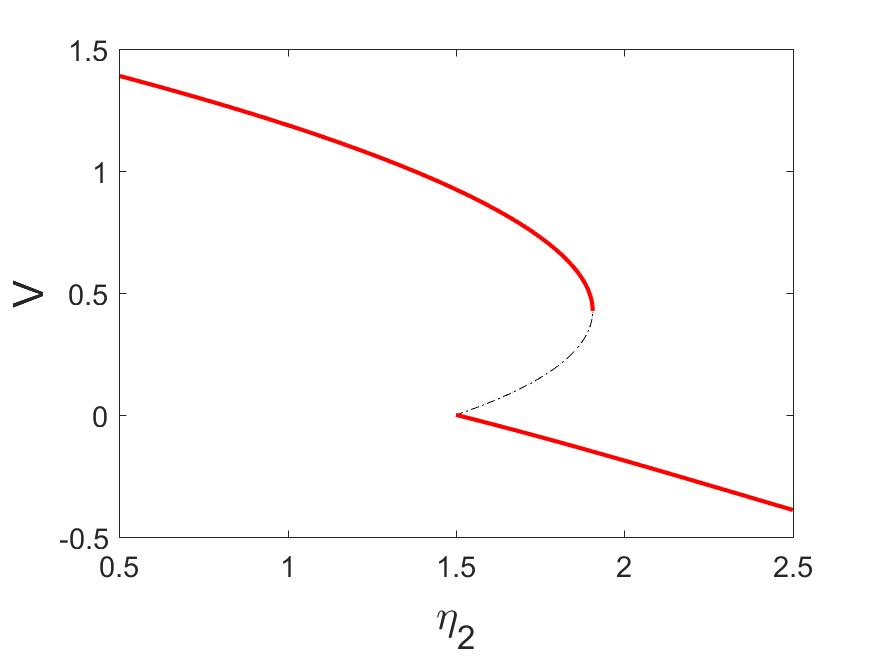
\includegraphics[width=\linewidth]{intro/V_bif.jpg}
  \caption{$\eta_3=.375$}
\end{subfigure}%
\begin{subfigure}{.5\textwidth}
  \centering
  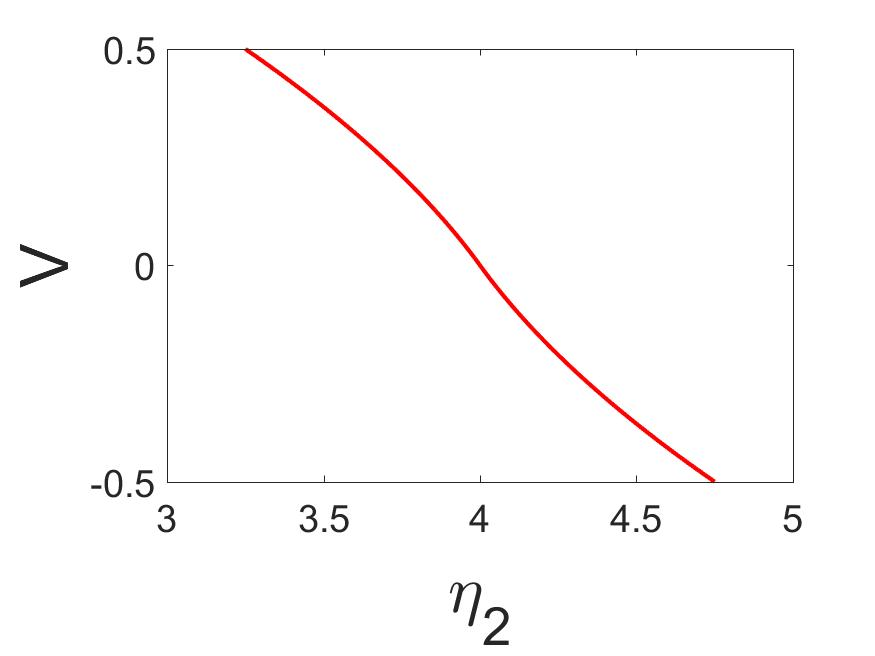
\includegraphics[width=\linewidth]{intro/V_bif_collapse.jpg}
  \caption{$\eta_3=1$}
\end{subfigure}
\begin{subfigure}{.5\textwidth}
  \centering
  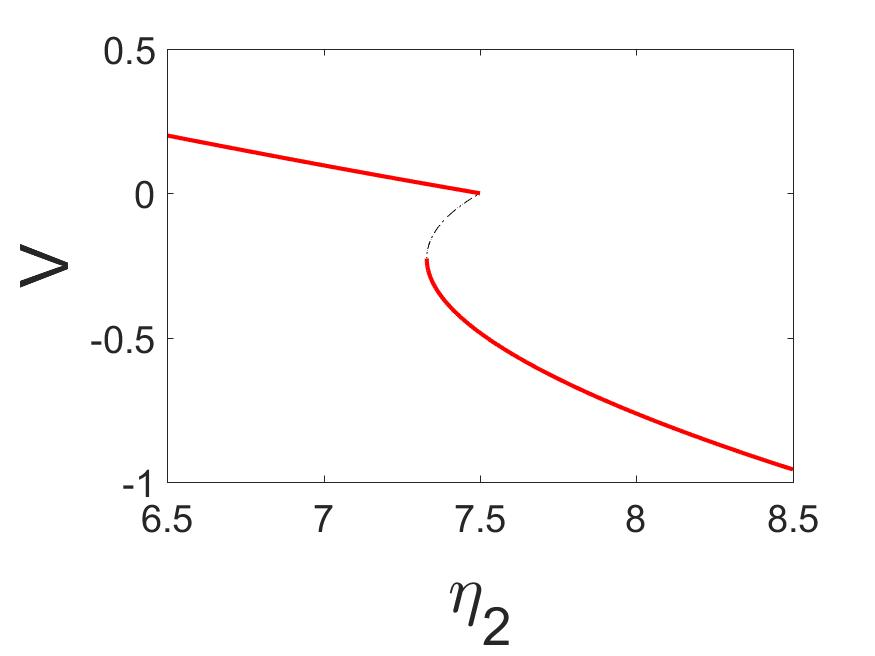
\includegraphics[width=\linewidth]{intro/V_bif_reverse.jpg}
  \caption{$\eta_3=1.875$}
\end{subfigure}
\caption{The choice in $\eta_3$ dictates the orientation of the problem, in each plot we have fixed $\eta_1=4$. The case for $\eta_3=1$ is special due to the two bifurcations overlapping and the unstable equilibrium vanishing.}
\label{fig:Stommel_bif_plots}
\end{figure}

Much is known about the Stommel model in the case where $\eta_2$ is fixed to be a constant value throughout the analysis but realistically this is not the case. In Rahmstorf \cite{rahmstorf2000thermohaline}, this parameter is described as the influx of freshwater into the Atlantic and the changing nature of $\eta_2$ is justified by a positive feedback loop for salinity that drives the THC to move high-salinity water towards deep oceans. This loop causes the abrupt smooth bifurcation but then afterwards, a salinity deficit causes the parameter to decrease back towards the non-smooth bifurcation.

This type of behavior is known as hysteresis, where there is some bi-stability region that the solution cycles through and hits both states of the equilibria. A similar analysis to the Stommel model's hysteresis can be found in Roberts \cite{roberts2017relaxation}. The phenomenon of hysteresis appears in many physical systems, for example Jung \cite{jung1990scaling}, Hohl \cite{hohl1995scaling} or Joshi \cite{joshi2005dynamical}. The smooth component of the hysteresis curve has been studied in a reduced one dimensional model, see Zhu \& Kuske \cite{zhu2015tipping}, we provide the other half of the analysis for the non-smooth component here.

\section*{Slowly Varying Tipping}
A system with a parameter known to cause a bifurcation will no longer admit a bifurcation in the standard sense when there is slow variation. Instead, these conditions give rise to a smooth but rapid change in the system's equilibria and where this occurs is called a tipping point.

A tipping point is a point that causes an abrupt smooth transition in dynamical behavior as the system moves into a qualitatively different state. The idea being that some positive feedback pushes change towards a different state once a critical point has been passed, for example with biological systems seen in Angeli \cite{angeli2004detection}. These are known to be caused by small changes in one or more parameters in the system. An analysis that lays the theoretic backing of slow varying tipping with algebraic bifurcations is found in Haberman \cite{haberman1979slowly}.

Tipping points have been discovered to occur in a wide variety of systems and have become a big staple in the study of areas like catastrophe theory and dynamical systems. They aid in predicting the future of a system and even could be a warning for irreversible change like in the case of the Stommel model. A tipping point thus shares similar characteristics of a bifurcation and typically occurs close to the standard bifurcation location.

An important paper that we extend the results of is Zhu \& Kuske \cite{zhu2015tipping} where work was done on the system

\begin{equation}\label{eq:intro_Zhueq}
\begin{aligned}
\dot{x} =& Da + k_0 +k_1 x + k_2 x^2,\\
\dot{a} =& -\epsilon,
\end{aligned}
\end{equation}

where $\mu\ll 1$. This system is a slowly varying quadratic differential equation containing a smooth saddle-node bifurcation and appears in many physical problems like Erneux \cite{erneux1989jump}. A major result from \cite{zhu2015tipping} is that the solution and tipping point for \eqref{eq:intro_Zhueq} have the form

\begin{equation}\label{eq:intro_Zhuairy}
x\sim \frac{1}{|k_2|}\left(\frac{k_1}{2}+\left(\frac{D|k_2|}{\epsilon}\right)^{1/3}\right)\frac{Ai'\left([D|k_2|\epsilon]^{-2/3}\left(\frac{k_1^2}{4}+k_0|k_2|+D|k_2|a\right)\right)}{Ai\left([D|k_2|\epsilon]^{-2/3}\left(\frac{k_1^2}{4}+k_0|k_2|+D|k_2|a\right)\right)}
\end{equation}

\begin{equation}\label{eq:intro_Zhuresult}
a_{\text{tip}}=(D|k_2|)^{-1/3}a_{\text{Airy}}-\frac{a_s}{D}\quad \text{for} \quad a_s = k_0+\frac{k_1^2}{4|k_2|},
\end{equation}

with $Ai(\cdot)$ being the Airy function and $a_{\text{Airy}}=\epsilon^{2/3}\cdot(-2.33810\ldots)$ corresponding to the first zero of the Airy function. The tipping found in \eqref{eq:intro_Zhuresult} is a recurring tool for the work presented in this paper, even though we deal with a version of \eqref{eq:intro_Zhueq} that has a non-smooth bifurcation.

\begin{figure}[H]
\centering
\begin{subfigure}{.5\textwidth}
  \centering
  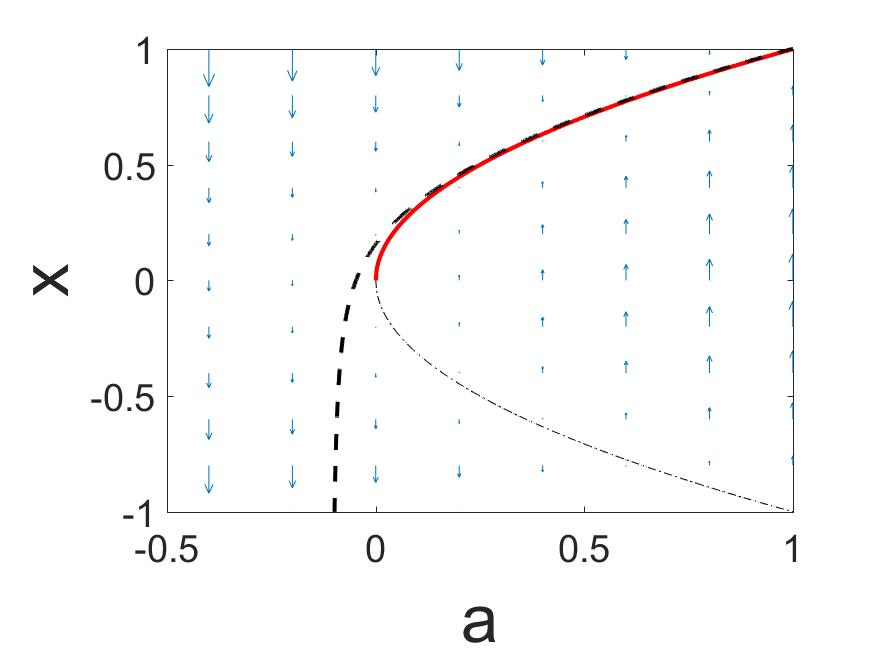
\includegraphics[width=\linewidth]{intro/saddlenode_tipping.jpg}
  \caption{}
\end{subfigure}%
\begin{subfigure}{.5\textwidth}
  \centering
  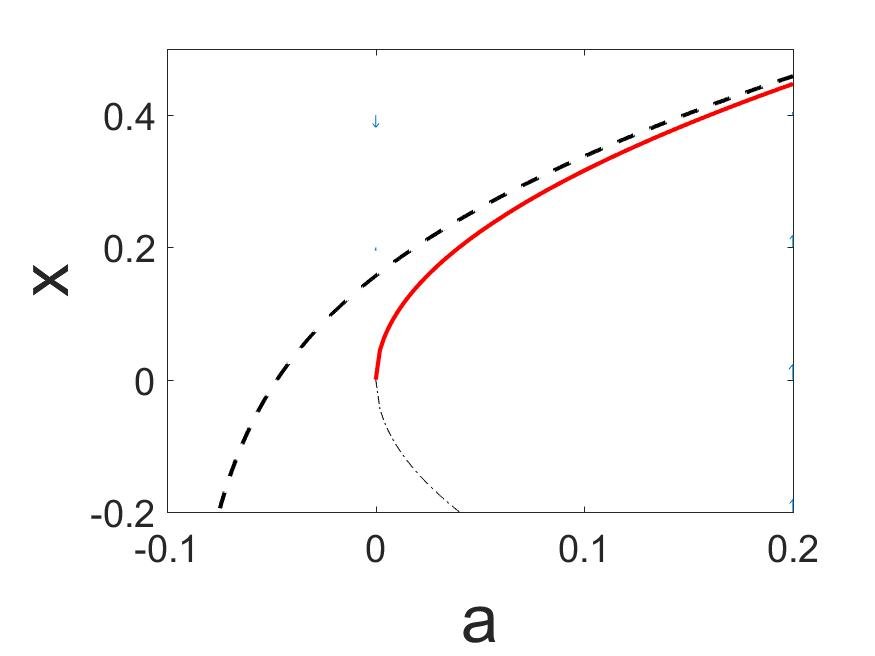
\includegraphics[width=\linewidth]{intro/saddlenode_tipping_zoom.jpg}
  \caption{}
\end{subfigure}
\caption{An example of tipping occurring in the saddle-node around the saddle-node bifurcation.}
\label{fig:intro_tipping}
\end{figure}


In figure~\ref{fig:intro_tipping} we show a numerical solution to the simple saddle-node system with tipping \eqref{eq:intro_Zhueq}. Here we have $D=1$, $k_0=k_1=0$ and $k_2=-1$ which is the model in \eqref{eq:intro_saddlenode} we saw earlier. The solution follows closely to the stable branch even after the bifurcation would have occurred, which is indicative of this delayed-typed behavior.


The task of finding where tipping occurs depends on the situation, but in general the approach is to search for when a solution to a problem fails or becomes uncontrollable. This happens when the solution fails to be real or when an exponential term grows too quickly, both of which we see throughout this paper.


\chapter{One Component Model}
\label{chap:oneD}
We consider a simpler system to give insight into the more complex two-dimensional Stommel model with the following one-dimensional model

\begin{equation}\label{eq:oneD_canonical}
\begin{aligned}
\dot{x}=-\mu+2|x|&-x|x|+A\sin(\Omega t),\\
\dot{\mu}=&-\epsilon,
\end{aligned}
\end{equation}

\begin{equation*}
x(0)=x^0,\quad\mu(0)=\mu^0,
\end{equation*}

where the constants are the slow variation rate of $\epsilon \ll 1$, the amplitude of oscillation $A$ and the frequency of oscillation $\Omega$. We also assume the initial conditions to be ${x^0=1-\sqrt{1+\mu^0}}$ and $\mu^0>\mu_{ns}$ which focuses our calculations on the lower equilibrium branch where $x<0$ and study nearby behavior. The value $\mu_{ns}$ refers to the non-smooth bifurcation and this is discussed below in \autoref{sec:oneD_static}.

The system \eqref{eq:oneD_canonical} is generalized from a basic model that contains both a smooth and non-smooth saddle-node bifurcation. This structure is similar to the Stommel model and hence a good model to test features like slow variation or oscillatory forcing. In each case, emphasis is put on the non-smooth component of the model to study the non-smooth bifurcation and the role it plays in the hysteresis curve we anticipate in the Stommel model.

\section{Static Bifurcations}
\label{sec:oneD_static}

The foundation to our understanding comes from the simplest structure lying within the canonical system \eqref{eq:oneD_canonical} which is the bifurcation structure. This means finding the general form for the equilibria in \eqref{eq:oneD_canonical} with $A=0$ and $\epsilon=0$, which is our basic model with a static $\mu$ and no forcing. As we have a fixed parameter value, we search for a point or set of points that the solution relaxes to as $t\to \infty$. We call these points the equilibrium points and they are either stable or unstable. But as we are considering all possible $\mu$, we want all of the equilibrium points for each $\mu$ and thus we call these the equilibrium branches.

To find all equilibrium branches, we search for when the solution has come to a rest, which is equivalent to setting the derivative of $x$ to zero. Thus we set \eqref{eq:oneD_canonical} to zero with

\begin{equation}\label{eq:oneD_static_equil}
0=-\mu +2|x|-x|x|.
\end{equation}

Solving \eqref{eq:oneD_static_equil} results in 3 solutions, the stability of each is characterized by small perturbations to the equilibrium either linearly growing or decaying. We denote the stable equilibria as $x_l$ and $x_u$ for the lower and upper branches respectively, and a single unstable middle branch, $x_{m}$. These are given by

\begin{equation*}
x_l=1-\sqrt{1+\mu},\quad x_u=1+\sqrt{1-\mu},\quad
x_{m}=1-\sqrt{1-\mu}.
\end{equation*}

We note that $x_l$ is valid for $\mu\ge 0$ and both $x_u$ and $x_{m}$ for $\mu\le 1$. Thus this system has a stable equilibrium for each value of the parameter and has a region of bi-stability for $0\le \mu\le 1$. The boundaries of this region are ${(\mu_{ns},x_{ns})=(0,0)}$ and $(\mu_{\text{smooth}},x_{\text{smooth}})=(1,1)$ which are the non-smooth and smooth saddle-node bifurcations respectively. Both are saddle-node due to pairs of equilibria annihilating at these locations which is shown in figure~\ref{fig:oneD_static_bifdiagram}.

\begin{figure}[H]
\centering
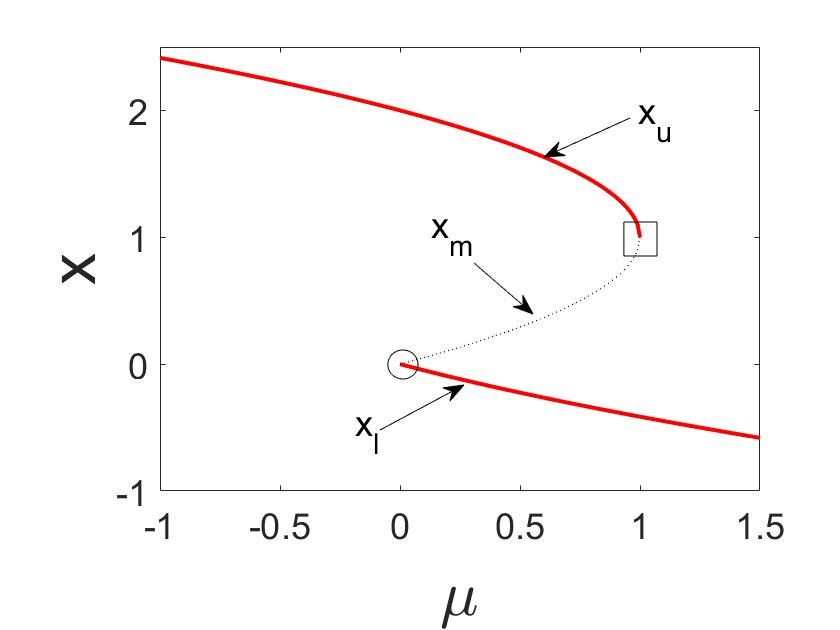
\includegraphics[width=.8\textwidth]{oneD/bif_diagram.jpg}
\caption{The one-dimensional bifurcation diagram with the upper and lower equilibrium branches as well as the unstable middle branch. The non-smooth bifurcation occurs at (0,0) denoted by the circle and the smooth bifurcation occurs at (1,1) by the box. }
\label{fig:oneD_static_bifdiagram}
\end{figure}


\section{Slowly Varying Bifurcation Parameter}
\label{sec:oneD_slow}

To develop a method for the slowly varying Stommel model, we consider \eqref{eq:oneD_canonical} with $\epsilon\ll 1$ and $A=0$. Under these conditions, $\mu(t)$ is a function of time and thus a bifurcation no longer occurs. Instead, it is expected that a tipping point occurs nearby the static bifurcation points as long as $\epsilon$ is small. Also, due to $\mu(t)$ being a function of time, we will find equilibria that are also functions in time, which we call pseudo-equilibira. The smooth case is well understood, see \cite{zhu2015tipping}, so we consider the behavior of the non-smooth bifurcation with $x<0$. From \cite{haberman1979slowly} as well as the smooth model \cite{zhu2015tipping}, it is common practice to rescale time in a model with slow variation to put the dynamics on the same order and allow for algebraic solutions to be found. Here the parameter $\mu(t)$ is slowly varying in time so it makes sense to rescale using this as our slow time, $\tau=\epsilon t$. Applying both $x<0$ and this slow time approach to the system \eqref{eq:oneD_canonical} then gives

\begin{equation}\label{eq:oneD_slow_scaled}
\begin{aligned}
\epsilon x_\tau=&-\mu(\tau)-2x+x^2,\\
\mu_\tau=&-1.
\end{aligned}
\end{equation}

A standard approach to extracting information out of complicated models is to find reduced equations by separating the behavior at each order of the slow time. This approach is known as using an asymptotic expansion and further details can be found in Murray's \textit{Asymptotic Analysis} \cite{murray2012asymptotic}. With $\epsilon$ being the small quantity that dictates our slow time, we choose to use an asymptotic expansion of $x$ with

\begin{equation}\label{eq:oneD_slow_asympexpan}
x(\tau)\sim x_0(\tau)+\epsilon x_1(\tau)+\epsilon^2 x_2(\tau)+O(\epsilon^3).
\end{equation}

This approach captures the slowly varying behavior of the solution in terms of this small quantity $\epsilon$ and aims to relate the slow variation to the solution. We substitute the expansion \eqref{eq:oneD_slow_asympexpan} into the scaled system \eqref{eq:oneD_slow_scaled} to get

\begin{equation*}
\epsilon {x_0}_\tau +\epsilon^2 {x_1}_\tau+\ldots= -\mu(\tau) -2x_0+x_0^2+\epsilon(-2x_1+2x_1x_0)+\epsilon^2(-2x_1+2x_2x_0+x_1^2)+\ldots
\end{equation*}

Once we separate the equations at each order of $\epsilon$, we find the following system of equations

\begin{align}
\label{eq:oneD_slow_outerO1}
O(1):& \quad 0=-\mu(\tau)-2x_0+x_0^2,\\
\label{eq:oneD_slow_outerO2}
O(\epsilon):& \quad 0=-{x_0}_\tau-2x_1+2x_1 x_0,\\
\label{eq:oneD_slow_outerO3}
O(\epsilon^2):& \quad 0=-{x_1}_\tau-2x_2+2x_2x_0+x_1^2.
\end{align}

Each of the equations \eqref{eq:oneD_slow_outerO1}-\eqref{eq:oneD_slow_outerO3} gives the respective order's pseudo-equilibrium. Thus we solve each equation progressively to find the terms of our asymptotic expansion \eqref{eq:oneD_slow_asympexpan} as

\begin{equation}\label{eq:oneD_slow_outersoln}
x(t)\sim 1-\sqrt{1+\mu(t)}+ \frac{\epsilon}{4(1+\mu(t))}-\frac{3\epsilon^2}{32(1+\mu(t))^{5/2}}+O(\epsilon^3).
\end{equation}

We call \eqref{eq:oneD_slow_outersoln} the outer solution as it approximates the solution well for values of $x(t)$ away from the bifurcation value $\mu_{ns}$. But since the dynamics of the system \eqref{eq:oneD_canonical} change at $x=0$ due to the non-smooth bifurcation of the underlying static system, this solution is valid only for $x<0$ and $\mu>0$.


It is a key assumption of an asymptotic expansion that the terms are clearly separated by order of $\epsilon$. We observe a scaling of $\mu$ and $x$ for which \eqref{eq:oneD_slow_outersoln} is no longer valid under this assumption of order separation, here when $x_0\sim \epsilon x_1$, which occurs for $\mu\sim O(\epsilon)$. We conduct a simple scale analysis to determine the appropriate scaling for the local analysis about $x=0$. Hence we consider the general scales

\begin{equation*}
x=\epsilon^\alpha y,\quad \mu = \epsilon^\beta m,
\end{equation*}

with $\alpha>0$ and $\beta>0$ for an inner scaling. We apply these local variables in \eqref{eq:oneD_canonical} to give the system

\begin{equation}\label{eq:oneD_slow_scalesearch}
\begin{aligned}
\epsilon^\alpha \dot{y}=&-\epsilon^\beta m +\epsilon^\alpha 2|y|-\epsilon^{2\alpha}y|y|,\\
 \epsilon^\beta \dot{m}=&-\epsilon.
\end{aligned}
\end{equation}

We balance the leading order terms $\epsilon^\alpha\dot{y}$ with $\epsilon^\beta m$ to give $\alpha=\beta$. But the equation for $m$ calls for $\beta=1$, thus we have the scaling for the local analysis

\begin{equation}\label{eq:oneD_slow_scales}
x=\epsilon y,\quad \mu=\epsilon m.
\end{equation}

We have found that the scalings in \eqref{eq:oneD_slow_scales} apply to all $x$ and thus we consider the region of $x>0$. Substituting the local variables \eqref{eq:oneD_slow_scales} into the original model \eqref{eq:oneD_canonical} we find the following inner system for the region of $x>0$

\begin{equation}\label{eq:oneD_slow_innereq}
\begin{aligned}
\dot{y}=&-m(t)+2 y-\epsilon y^2,\\
\dot{m}=&-1.
\end{aligned}
\end{equation}

We recall that we are searching for a link between $y$ and $m$, and from \cite{haberman1979slowly} we use that it is then convenient to change the differentiation on $y$ to be with respect to the parameter $m$. This incorporates the behavior of $m(t)$ directly into the equation we solve and gives us a direct method for finding the tipping point. Then the leading order equation is

\begin{equation}\label{eq:oneD_slow_innerm}
y_m = m-2y.
\end{equation}

The leading order solution to \eqref{eq:oneD_slow_innerm} is found explicitly as follows

\begin{equation*}
y(m) = C e^{-2m}+\frac{m}{2}-\frac{1}{4}+O(\epsilon).
\end{equation*}

With the inner solution found in terms of the parameter $m$, we write this in terms of the original variables with

\begin{equation}\label{eq:oneD_slow_innersoln}
x(t)\sim Ce^{-2\mu(t)/\epsilon}+\frac{\mu(t)}{2}+O(\epsilon).
\end{equation}

Since the solution \eqref{eq:oneD_slow_innersoln} behaves exponentially, the tipping point, $\mu_{\text{slow}}$, occurs when the exponential term begins to grow rapidly. Here we consider tipping to occur when the solution becomes $O(1/\epsilon)$. Thus we find the tipping point $\mu_{\text{slow}}$ to take the form

\begin{equation}\label{eq:oneD_slow_tipping}
\mu_{\text{slow}}= \frac{1}{2}\epsilon \log (\epsilon).
\end{equation}

Thus we have the tipping point for the slowly varying model. Notice that for small values of $\epsilon$, $\mu_{\text{slow}}<\mu_{ns}$ and this is consistent with considering the inner equation \eqref{eq:oneD_slow_innereq} for the region $x>0$ as we found in the analysis. Thus we find that a slowly varying bifurcation parameter causes a delay in the rapid transition to the upper branch and we expect the solution to remain near the lower branch for longer than in the static problem. In terms of hysteresis, then slow variation allows for a longer period before the states switch from the lower to the upper branch.

In figure~\ref{fig:oneD_slow_numerics} (a,b), an example of this tipping is shown for a choice in $\epsilon$ along with the standard bifurcation diagram where (c) demonstrates the tipping approximation across a range of $\epsilon$. The concavities match as well as clear agreement in the estimation of the tipping point as $\epsilon$ goes to 0.

\begin{figure}[H]
\centering
\begin{subfigure}{.5\textwidth}
 \centering
 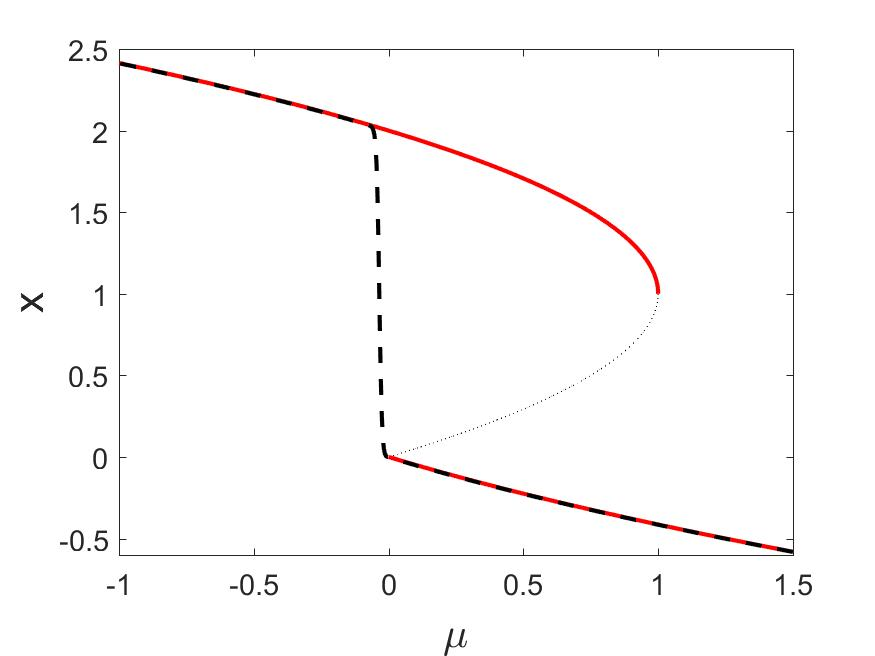
\includegraphics[width=\linewidth]{oneD/slow_bif_diagram.jpg}
 \caption{}
\end{subfigure}%
\begin{subfigure}{.5\textwidth}
 \centering
 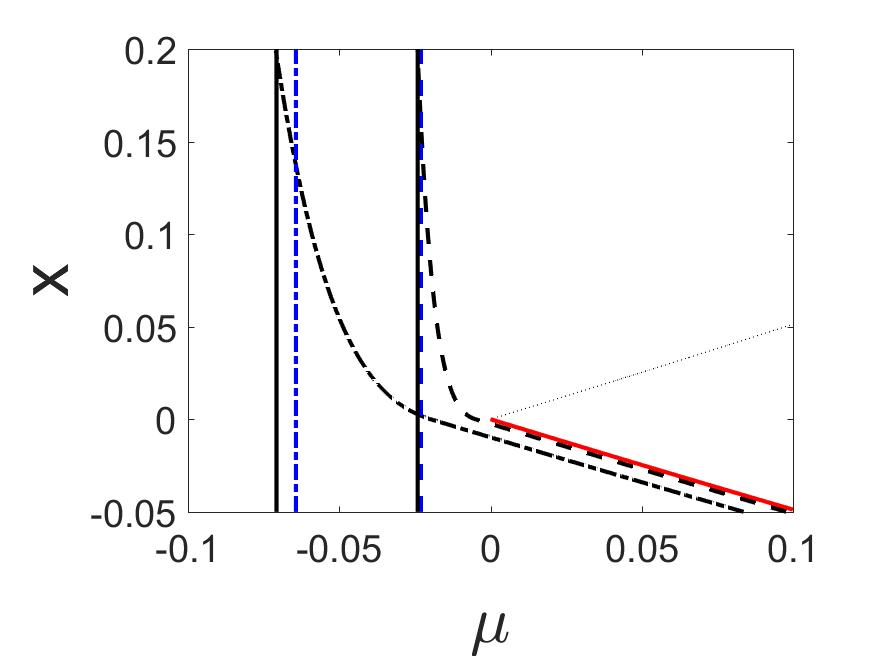
\includegraphics[width=\linewidth]{oneD/slow_bif_diagram_zoom.jpg}
 \caption{}
\end{subfigure}
\begin{subfigure}{.5\textwidth}
\centering
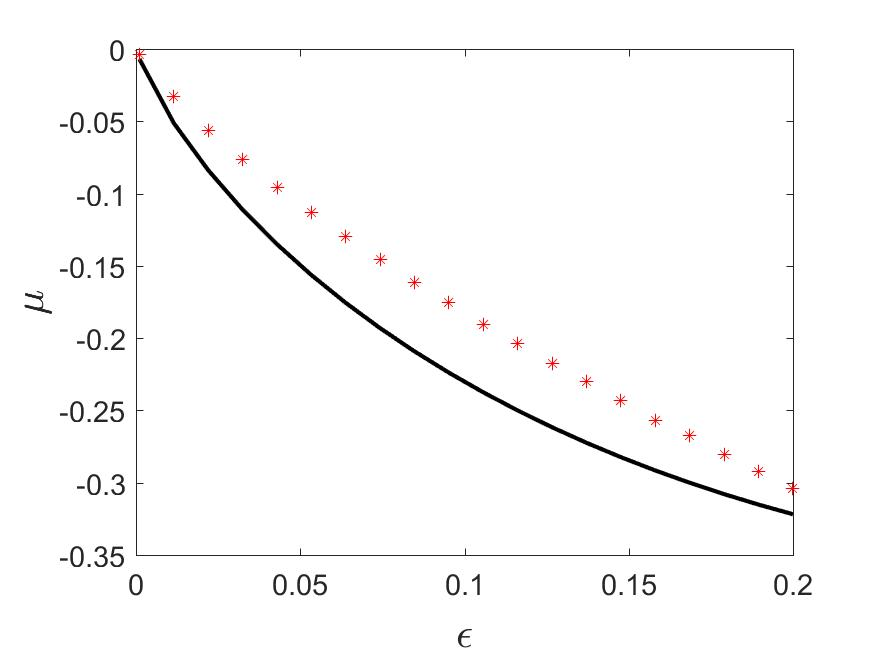
\includegraphics[width=\linewidth]{oneD/slow_epscomp.jpg}
\caption{}
\label{fig:oneD_slow_comp}
\end{subfigure}
\caption{In (a) the numerical solution (black dotted line) to \eqref{eq:oneD_canonical} is given with $A=0$ and $\epsilon=.01$. The bifurcation plot is overlayed for convenience. In (b) a zoom in of what happens near the non-smooth bifurcation. The solid vertical line (black) is the numerical tipping for which we use the criteria $x>.5$ and the dotted vertical line (blue) is the tipping estimate. In (c) a range of $\epsilon$ and their corresponding tipping (red stars) are compared to our estimate (solid black line) from \eqref{eq:oneD_slow_tipping}.}
\label{fig:oneD_slow_numerics}
\end{figure}


\subsection{Stability}
From the static model we know our outer solution \eqref{eq:oneD_slow_outersoln} to be stable, but to verify that the inner solution \eqref{eq:oneD_slow_innersoln} is stable, we use a simple linear stability analysis on the inner system. Typically to do this, an analysis would be performed about an equilibrium to see if perturbations would grow or decay. But as this problem has a parameter that is allowed to vary, we instead must be careful to note the analysis must be done on the pseudo-equilibrium instead. In the first region of interest, $m(t)\ge 0$, the following inner equation and pseudo-equilibrium, $z^0(t)$, hold below the axis

\begin{equation}\label{eq:oneD_slow_stability1}
\dot{y}=-m(t)-2y=f(t,y), \quad z^0(t)=-\frac{m(t)}{2}.
\end{equation}

We then consider simple perturbations about the pseudo-equilibrium in \eqref{eq:oneD_slow_stability1} with

\begin{equation*}
y(t)=z^0(t)+u(t), \quad \lVert u(t) \rVert \ll 1.
\end{equation*}

Normally a Taylor expansion would result in expressing the perturbations with their own equation that we could use to determine stability. Since $z^0(t)$ is not fixed, we must consider its contribution to the derivative in this region of the parameter space with $m(t)\ge 0$. Thus we find

\begin{equation}\label{eq:oneD_slow_stability2}
\begin{aligned}
\dot{y} =& \,\dot{z}^0+\dot{u},\\
\dot{z}^0= & \begin{cases}
\frac{1}{2} & m(t)>0,\\
0 & m(t)=0.
\end{cases}
\end{aligned}
\end{equation}

Now we apply the standard Taylor expansion to see the behavior of these perturbations and with the contributions in \eqref{eq:oneD_slow_stability2}, the inner equation \eqref{eq:oneD_slow_stability1} becomes

\begin{equation}\label{eq:oneD_slow_perturbeq}
\begin{aligned}
\dot{y}=& f(t,z^0)+f_y(t,z^0)(y-z^0)
= f_y(t,z^0)u,\\
\dot{u}=&\begin{cases}
-\frac{1}{2}-2u, & m(t)>0,\\
-2u, & m(t)=0.
\end{cases}
\end{aligned}
\end{equation}

If this were the static parameter problem, we would always have the second case in \eqref{eq:oneD_slow_perturbeq}, which is always stable due to the sign. Since we allow for a varying parameter, we learn that the solution is attracted to just below the pseudo-equilibrium $z^0(t)$. As this system always experiences the critical point $m=0$ due to the continuous decrease in $m(t)$, the slowly varying parameter eventually acts like the static parameter in \autoref{sec:oneD_static}. Hence we have that for $x<0$, the pseudo-equilibrium is hyperbolic and asymptotically stable. But here there is a critical point at $(\mu_{ns},x_{ns})=(0,0)$ which corresponds to a non-hyperbolic equilibrium point. Generally, non-hyperbolic behavior signals equilibrium structure to be changing. Here, this signals a transition in behavior for $x>0$ and helps identify that the tipping occurs here.

For the second region of interest, $m(t)<0$, we found a solution that had the following inner equation which has the pseudo-equilibrium above the axis with

\begin{equation}\label{eq:oneD_slow_innerstability}
\dot{y}=-m(t)+2y, \quad z^0(t) = \frac{m(t)}{2}.
\end{equation}

But we find a contradiction from \eqref{eq:oneD_slow_innerstability}, here $m(t)<0$ yet the solution of this region is above the axis $x=0$. Thus we may conclude that this inner equation has no equilibrium in this region and further verifies that the critical point $(\mu_{ns},x_{ns})$ was non-hyperbolic and tipping occurs for $m(t)<0$.

\section{High Frequency Oscillatory Forcing}
\label{sec:oneD_highfreqosc}

To understand the oscillatory forcing in the Stommel model, consider the canonical system \eqref{eq:oneD_canonical} with $A\sim O(1)$, $\Omega\gg 1$ and $\epsilon=0$, which gives high frequency oscillatory forcing in the system. Under these conditions, we have a static parameter and for each parameter value there is oscillatory forcing with solutions characterized by oscillations about a fixed point. Thus we should expect to find a bifurcation influenced by oscillations occurring under these conditions. Here we develop a method to find oscillatory solutions to determine what the effect of oscillatory forcing has on the bifurcation of \eqref{eq:oneD_canonical}. In \autoref{sec:oneD_slow}, we focused only on the slowly varying dynamics but here we have both a slow time scale $t$ and a fast time scale $T=\Omega t$. This naturally suggests a multiple scales approach where we search for a solution that is dependent on both of these scales, $x(t)=x(t,T)$. This method is commonly used in problems that have behavior observable on multiple scalings, and we use it here to find a way to accurately analyze each scale and effectively combine their behavior into a single unifying solution. Further discussion on this method can be found in \cite{sanchez1996method}.

Recall that our focus is on the non-smooth behavior and hence we restrict the solution to follow along the lower stable equilibrium branch where $x<0$. Using this multiple scales approach, our canonical system \eqref{eq:oneD_canonical} has the following form

\begin{equation}\label{eq:oneD_osc_multiscale}
x_T+\Omega^{-1}x_t=\Omega^{-1}\left(-\mu-2x+x^2+A\sin(T)\right).
\end{equation}

In \eqref{eq:oneD_osc_multiscale}, the small quantity $\Omega^{-1}$ appears which suggests an asymptotic expansion in powers of this quantity

\begin{equation}\label{eq:oneD_osc_asymptotic}
x(t,T)\sim x_0(t,T)+\Omega^{-1}x_1(t,T)+\Omega^{-2}x_2(t,T)+O(\Omega^{-3}).
\end{equation}

Substituting \eqref{eq:oneD_osc_asymptotic} into \eqref{eq:oneD_osc_multiscale}, we find

\begin{equation*}
{x_0}_T+\Omega^{-1}{x_0}_t+\Omega^{-1}{x_1}_T+\ldots=\Omega^{-1}(-\mu-2x_0+x_0^2+A\sin(T))+\Omega^{-2}(-2x_1+2x_1x_0)+\ldots
\end{equation*}

Here we separate by each order of $\Omega$ to find the following system of reduced equations

\begin{align}
\label{eq:oneD_osc_outerO1}
O(1):& \quad {x_0}_T=0, \\
\label{eq:oneD_osc_outerO2}
O(\Omega^{-1}):& \quad {x_1}_T+{x_0}_t =-\mu-2x_0+x_0^2+A\sin(T),\\
\label{eq:oneD_osc_outerO3}
O(\Omega^{-2}):& \quad {x_2}_T + {x_1}_t= -2x_1+2x_0 x_1.
\end{align}

With an equation at each order, we must able to solve each to proceed to the next but we must also further restrict our solution from having resonant or linearly growing terms to prevent any multiplicity or exponential growth. This assures that the terms in the asymptotic expansion are compatible with one another and we find a robust solution. A common method to guarantee compatible solutions with sublinear growth at each order is the Fredholm alternative. This provides a solvability condition for each equation of the form ${x_i}_T=R_i(t,T)$ with

\begin{equation*}
\lim\limits_{T\to\infty}\frac{1}{T}\int_0^T R_i(t,u)\,du=0,
\end{equation*}

although for this system we consider the periodic form of the Fredholm alternative

\begin{equation} \label{eq:Fredholm}
\frac{1}{2\pi}\int_0^{2\pi}R_i(t,T)\,dT=0.
\end{equation}

Both the general and periodic form of the Fredholm alternative have been well studied and a more theoretic approach to the periodic version is discussed in Bensoussan's \textit{Asymptotic analysis for periodic structures} \cite{bensoussan2011asymptotic}. From \eqref{eq:oneD_osc_outerO1}, we learn the leading order term is only dependent on the slow time, $x_0=x_0(t)$. Applying the Fredholm alternative \eqref{eq:Fredholm} to \eqref{eq:oneD_osc_outerO2} gives

\begin{equation}\label{eq:oneD_osc_outerO2soln}
\begin{aligned}
0=&\frac{1}{2\pi}\int_0^{2\pi} -{x_0}_t(t) -\mu -2x_0(t)+x_0(t)^2+A\sin(T)\,dT ,\\
{x_0}_t=& -\mu -2x_0+x_0^2 ,\\
{x_1}_T =& A\sin(T).
\end{aligned}
\end{equation}

Solving for the equilibrium solution of \eqref{eq:oneD_osc_outerO2soln} leads to the leading order solution, $x_0$, and also allows us to partially solve for the first correction term $x_1$ with

\begin{equation*}
\begin{aligned}
x_0 =& 1-\sqrt{1+\mu},\\
x_1(t,T) =& v_1(t) - A\cos(T).
\end{aligned}
\end{equation*}

Repeating this procedure in \eqref{eq:oneD_osc_outerO3}, as shown in \autoref{app:oneD}, results in the expansion \eqref{eq:oneD_osc_asymptotic} written in the original variables

\begin{equation}\label{eq:oneD_osc_outersoln}
x\sim 1-\sqrt{1+\mu}-\Omega^{-1} A \cos(\Omega t)+O(\Omega^{-2}).
\end{equation}

Once again, the explicit outer solution \eqref{eq:oneD_osc_outersoln} performs well for $x$ away from the axis $x=0$, we search for when the assumptions of the asymptotic series fail indicating where an inner analysis is needed. This is when $x_0\sim \epsilon x_1$ which occurs for $\mu\sim O(\Omega^{-1})$.

We consider a general scaling for $x=\Omega^{-\alpha}y$ and $\mu = \Omega^{-\beta}m$ where $\alpha>0$ and $\beta>0$ allows for an inner equation. Applying these local variables to \eqref{eq:oneD_canonical} results in

\begin{equation}\label{eq:oneD_osc_generalinner}
\dot{y} = -\Omega^{\alpha-\beta}m+2|y|-\Omega^{-\alpha}y|y|+\Omega^{\alpha}A\sin(\Omega t)
\end{equation}

In this local system \eqref{eq:oneD_osc_generalinner}, we find similar behavior occurring across multiple scales and thus we are able to use the same time scales from the outer analysis, $t=t$ and $T=\Omega t$. Then we have that $y(t)=y(t,T)$ and hence a similar multiple scales argument in \eqref{eq:oneD_osc_generalinner} leads to

\begin{equation}\label{eq:oneD_osc_innergeneralmulti}
y_T+\Omega^{-1}y_t = - \Omega^{\alpha-\beta-1}m+\Omega^{-1}2|y|-\Omega^{-\alpha-1}y|y|+\Omega^{\alpha-1}A\sin(T).
\end{equation}

With a standard balancing argument between the leading order terms in \eqref{eq:oneD_osc_innergeneralmulti} $y_T$ and $\Omega^{\alpha-1} A\sin(T)$, we see that $\alpha=1$. But we also want to see the terms $\Omega^{\alpha-\beta-1}m$ balance with $\Omega^{-1}2|y|$, which gives us that $\beta=1$ as well. This results in the inner equation

\begin{equation}\label{eq:oneD_osc_naivemultiscales}
y_T+\Omega^{-1}y_t = \Omega^{-1}\left(-m+2|y|\right)-\Omega^{-2}y|y|+A\sin(T).
\end{equation}

Similarly to the outer equation, we approximate the solution with an asymptotic expansion in terms of $\Omega^{-1}$ 

\begin{equation}\label{eq:oneD_osc_innerasymptotic}
y(t,T)\sim y_0(t,T)+\Omega^{-1}y_1(t,T)+O(\Omega^{-2}).
\end{equation}

Substituting the expansion \eqref{eq:oneD_osc_innerasymptotic} into the inner equation \eqref{eq:oneD_osc_naivemultiscales} we find

\begin{equation*}
{y_0}_T+\Omega^{-1}{y_0}_t+\Omega^{-1}{y_1}_T+\ldots =\begin{aligned}[t]\Omega^{-1}&(-m+2|y_0+\Omega^{-1}y_1+\ldots|)+A\sin(T)\\
&+\Omega^{-2}(y_0+\Omega^{-1}y_1+\ldots)|y_0+\Omega^{-1}y_1+\ldots|
\end{aligned}
\end{equation*}

Here we then find the following system of equations at each order of $\Omega$

\begin{align}
\label{eq:oneD_osc_innerO1}
O(1):\quad & {y_0}_T = A\sin(T),\\
\label{eq:oneD_osc_innerO2}
O(\Omega^{-1}):\quad & {y_1}_T+{y_0}_t = -m+2|y_0|.
\end{align}

Solving the leading order equation \eqref{eq:oneD_osc_innerO1} gives that the leading order term has the form, $y_0(t,T)=v_0(t)-A\cos(T)$. But applying the Fredholm alternative \eqref{eq:Fredholm} to \eqref{eq:oneD_osc_innerO2} leads to

\begin{equation}\label{eq:oneD_osc_integral}
{v_0}_t(t)=-m+\frac{1}{\pi}\int_0^{2\pi} |v_0(t)-A\cos(T)|\,dT.
\end{equation}

Here we must consider two cases of $v_0(t)$ that determine the nature of this integrand, Case I: if $v_0(t)$ is large enough to keep $y_0$ from ever changing signs and Case II: if $v_0(t)$ is too small and $y_0$ changes sign. In figure~\ref{fig:oneD_osc_cases} we show the range of each case where the region on the right is following under Case I, the green dotted vertical line defining the parameter range between the cases, the middle region for Case II and the blue vertical line giving the bifurcation, $\mu_{\text{osc}}$, which is determined below.

\begin{figure}[H]
\centering
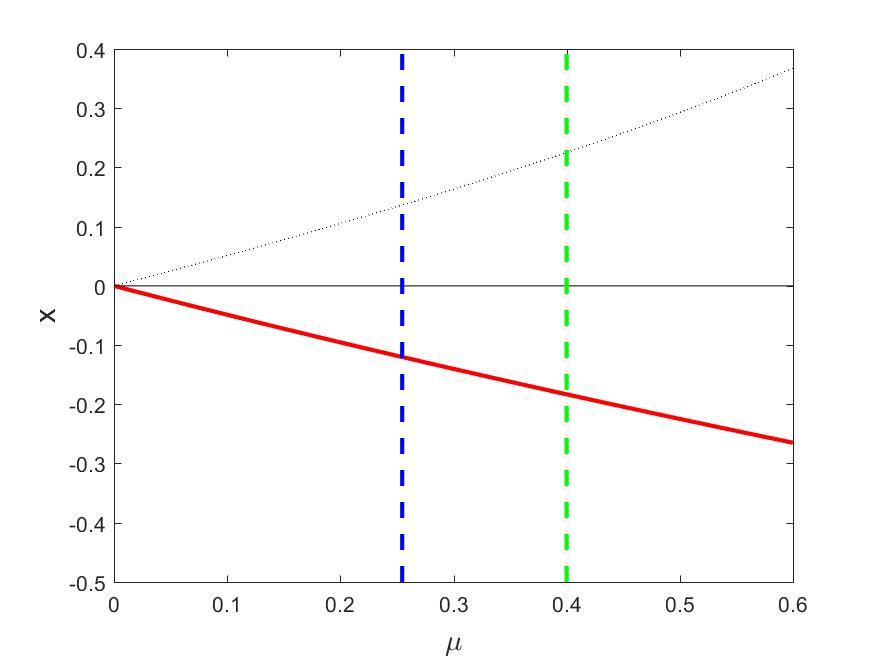
\includegraphics[width=.7\textwidth]{oneD/osc_cases.jpg}
\caption{The parameter ranges for each case is shown here with $A=2$. For reference, the original bifurcation diagram is overlayed.}
\label{fig:oneD_osc_cases}
\end{figure}

\subsection{Case I: $v_0(t) \le -|A|$}
\label{subsec:oneD_osc_CaseI}

We call this the entirely below axis case as the solution stays far from the axis $x=0$ for most of the oscillation and thus the behavior is not influenced by the non-smooth dynamics. We do not expect to see the bifurcation occur under these conditions but instead we find the parameter range for the cases. Here the integral in equation \eqref{eq:oneD_osc_integral} is straightforward to evaluate as $v_0(t)$ is a constant with respect to the fast time $T$, thus we find the inner equation and equilibrium

\begin{equation*}
{v_0}_t=-m-2v_0,\quad v_0=-\frac{m}{2}.
\end{equation*}

This gives the leading order equilibrium solution with oscillations to the local variables for this case which we write in the original variables

\begin{equation}\label{eq:oneD_osc_caseIsoln}
\begin{aligned}
y(t,T)\sim& -\frac{m}{2}-A\cos(T)+O(\Omega^{-1}),\\ 
x(t)\sim& -\frac{\mu}{2}-\Omega^{-1} A\cos(\Omega t)+O(\Omega^{-2}).
\end{aligned}
\end{equation}

The condition $v_0(t)\le -|A|$ combined with the equilibrium allows us to establish when \eqref{eq:oneD_osc_caseIsoln} holds

\begin{equation}\label{eq:oneD_osc_caseboundary}
\mu\ge \frac{2|A|}{\Omega}.
\end{equation}

Following the equilibrium to \eqref{eq:oneD_osc_caseboundary} leads us to Case II where the oscillations cross the axis and the assumptions of this case no longer hold.

\subsection{Case II: $|v_0(t)|< |A|$}
\label{subsec:oneD_osc_CaseII}

We call this the crossing case; here the equilibrium is small enough that the oscillations can now push the solution above the axis. Under these conditions, the solution spends time near the axis $x=0$ and thus experiences the non-smooth influence. As the crossing continues, the non-smooth behavior drives the solution to gradually grow and thus we expect to find the bifurcation here. From \eqref{eq:oneD_osc_caseboundary}, we have a range of $\mu$ for when this case applies, $\mu<\frac{2|A|}{\Omega}$. But the integrand in \eqref{eq:oneD_osc_integral} is non-trivial when $|v_0(t)|<|A|$. In order to deal with the sign changing inside the integral, we break the integration into regions based on sign. Recall that we are searching for equilibrium behavior, and so we may make the assumption that we are dealing with a fixed value of $v_0$ such that $|v_0|\le |A|$. In figure~\ref{fig:oneD_osc_t1t2_graphic} we observe the function that we are integrating.

\begin{figure}[H]
\centering
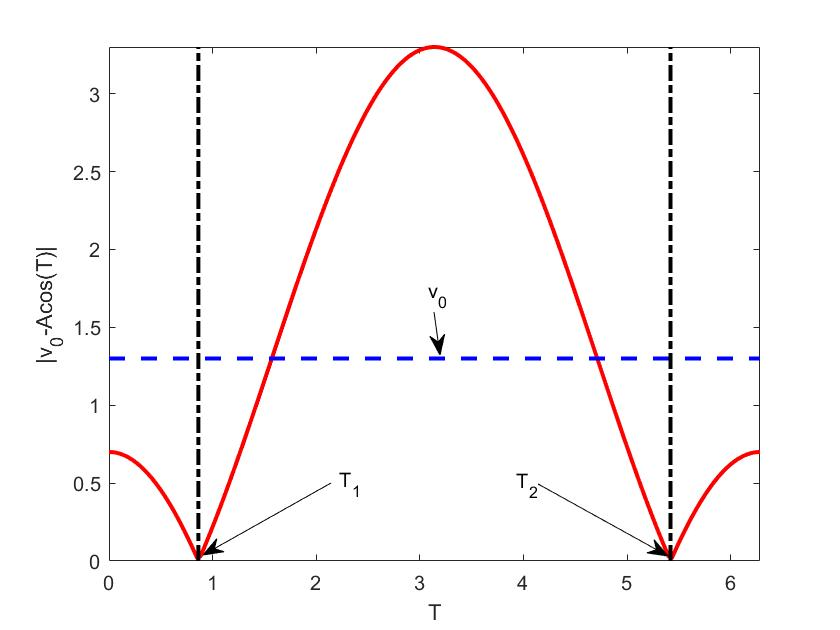
\includegraphics[width=0.7\textwidth]{oneD/t1t2_graphic.jpg}
\caption{The non-smooth function $|y_0|=|v_0-A\cos(T)|$ that we integrate is shown as the solid red line. We also show an example of $v_0$ as a horizontal blue dotted line. Here the value of $|v_0|\le|A|$, which causes kinks to appear at the roots of $|y_0|$: $T_1$ and $T_2$ respectively. These are the vertical black dashed dotted lines. }
\label{fig:oneD_osc_t1t2_graphic}
\end{figure}

We now consider the following roots of the integrand with 

\begin{equation*}
T_1=\arccos (v_0/A),\qquad T_2= 2\pi - \arccos (v_0/A).
\end{equation*}

Here we notice $0<T_1<T_2<2\pi$ and that the sign of the integrand stays the same on each interval. We only assume that the interval $[0,T_1]$ is following the solution while the center is still negative, thus the integrand will also be negative. From this, the integral is

\begin{equation}\label{eq:oneD_osc_expandedintegral}
\begin{aligned}
\int_0^{2\pi}|v_0-A\cos(T)|\,dT=&-\int_0^{T_1}(v_0-A\cos(T))\,dT+\\
&\int_{T_1}^{T_2}(v_0-A\cos(T))\,dT-\int_{T_2}^{2\pi}(v_0-A\cos(T))\,dT.
\end{aligned}
\end{equation}

Evaluating \eqref{eq:oneD_osc_expandedintegral} and using a trig identity, $\sin(\arccos(x))=\sqrt{1-x^2}$, we find the integral to be

\begin{equation*}
\int_0^{2\pi}|v_0-A\cos(T)|\,dT=\frac{2}{\pi}\left(\arcsin(v_0/A)v_0+\sqrt{A^2-v_0^2}\right).
\end{equation*}

Now, we notice that our argument above is simple for $v_0$ in equilibrium, but we have used a multiple scales approach for our fast time with $t\ll T$ implying that $v_0(t)$ is approximately fixed over $T\in [0,2\pi]$. This holds true due to having a high frequency $\Omega$ and otherwise would not be a valid approximation. Thus we can evaluate \eqref{eq:oneD_osc_integral} to find the inner equation 

\begin{equation}\label{eq:oneD_osc_caseIIexact}
{v_0}_t=-m+\frac{4}{\pi}\left(\arcsin(v_0/A)v_0+\sqrt{A^2-v_0^2}\right).
\end{equation}

But in its current form, \eqref{eq:oneD_osc_caseIIexact} restricts an explicit form for $v_0(t)$, so we use a quadratic Taylor approximation to be able to solve this equation explicitly

\begin{equation}\label{eq:oneD_osc_caseIItaylor}
{v_0}_t \approx -m + \frac{4|A|}{\pi} + \frac{2}{\pi |A|}v_0^2,
\end{equation}

which has the following equilibrium with positive constant $C$

\begin{equation}\label{eq:oneD_osc_caseIIequil}
v_0=-C\sqrt{m-\frac{4|A|}{\pi}}.
\end{equation}

Thus we have the leading order inner equilibrium \eqref{eq:oneD_osc_caseIIequil} and we write this back in the original variables with

\begin{equation}\label{eq:oneD_osc_innersoln}
\begin{aligned}
y\sim& -C\sqrt{m-\frac{4|A|}{\pi}}-A\cos(T)+O(\Omega^{-1}),\\ 
x(t)\sim& -C\sqrt{\Omega \left(\mu-\frac{4|A|}{\pi \Omega}\right)}-\Omega^{-1} A\cos(\Omega t)+O(\Omega^{-2}).
\end{aligned}
\end{equation}

It then is clear that the bifurcation, $\mu_{\text{osc}}$, occurs when \eqref{eq:oneD_osc_innersoln} fails to be real valued. Thus we find $\mu_{\text{osc}}$ to take the form

\begin{equation}\label{eq:oneD_osc_bif}
\mu_{\text{osc}}=\frac{4|A|}{\pi \Omega}.
\end{equation}

From the result \eqref{eq:oneD_osc_bif}, we gather that the oscillatory forcing in the system causes the bifurcation to occur sooner, $\mu_{\text{osc}}>\mu_{ns}$, and this is controlled by the size of $A$ and $\Omega$. This should be expected as the model experiences the non-smooth behavior sooner in $\mu$ with the oscillations, but we can see as $\Omega\to\infty$ then $\mu_{\text{osc}}\to\mu_{ns}$. This effect is contrary to the slow variation where the solution experienced a delayed tipping, $\mu_{\text{slow}}<\mu_{ns}$. This also indicates that the region of bi-stability is shrunk with oscillatory forcing and thus can be used to eliminate the region entirely with $A$ and $\Omega$ chosen properly, effectively destroying any hysteresis. We compare our estimate to numerical results for varying sizes of $\Omega^{-1}$.

\begin{figure}[H]
\centering
\begin{subfigure}{.5\textwidth}
 \centering
 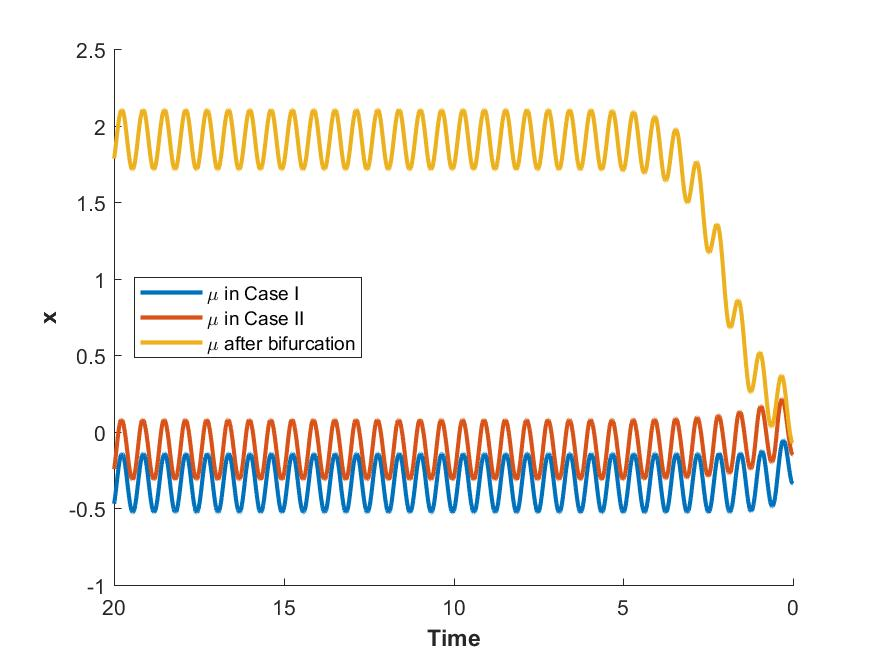
\includegraphics[width=\linewidth]{oneD/osc_timeseries.jpg}
 \caption{}
\end{subfigure}%
\begin{subfigure}{.5\textwidth}
 \centering
 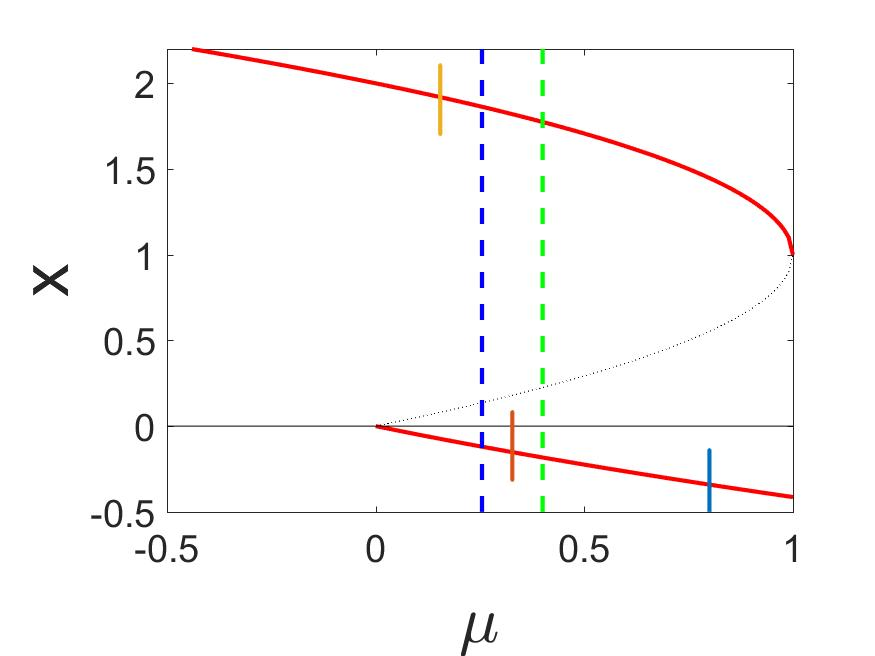
\includegraphics[width=\linewidth]{oneD/osc_bif_diagram.jpg}
 \caption{}
\end{subfigure}
\begin{subfigure}{.5\textwidth}
 \centering
 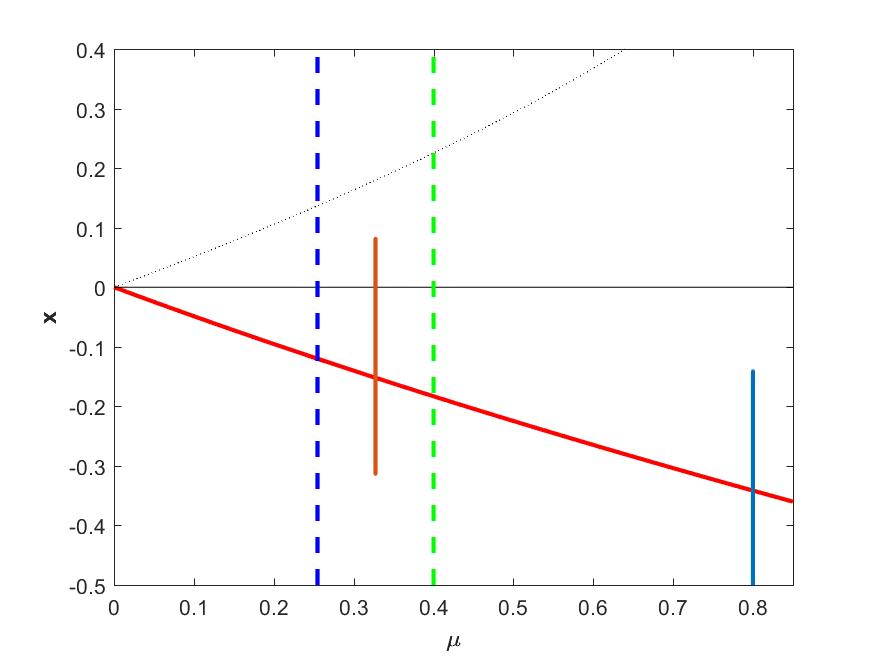
\includegraphics[width=\linewidth]{oneD/osc_bif_diagram_zoom.jpg}
 \caption{}
\end{subfigure}%
\begin{subfigure}{.5\textwidth}
\centering
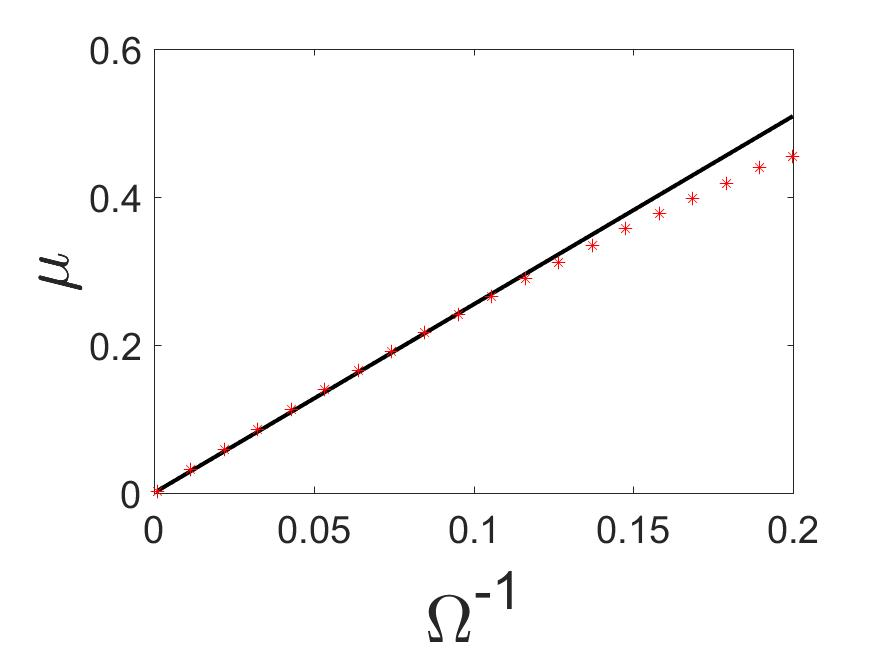
\includegraphics[width=\linewidth]{oneD/osc_Omegacomp.jpg}
\caption{}
\label{fig:oneD_osc_comp}
\end{subfigure}
\caption{In (a) the numerical time series solutions to \eqref{eq:oneD_canonical} are given from bottom to top with $\mu=\{.8,.33,.15\}$ in Case I, Case II and $\mu<\mu_{\text{osc}}$ in \eqref{eq:oneD_osc_bif} respectively with $A=2$, $\Omega=10$ and $\epsilon=0$. In (b) we show the time series on the bifurcation diagram. In (c), a zoom in closer to the non-smooth bifurcation, where the dotted vertical lines dictate the region between Case I and Case II (green) as well as the bifurcation estimate (blue) respectively. In (d) a range of $\Omega^{-1}$ and their corresponding numerical bifurcations (red stars) are compared to our estimate of the bifurcation (black solid line). We consider the numeric bifurcation to be when the solution has passed $x>.5$.}
\label{fig:oneD_osc_numerics}
\end{figure}

In figure~\ref{fig:oneD_osc_numerics} an example is shown of the effect oscillatory forcing has given a choice of $A$ and $\Omega$ with (a), (b) and (c), but (d) shows the bifurcation approximation across a range of $\Omega^{-1}$. There is an allowed range of $\Omega$ from our assumption of $\Omega \gg 1$ and in this region we see agreement. The concavity is well represented and the behavior as $\Omega^{-1}\to 0$ converges to the static bifurcation. Thus we expect that our methodology is valuable for the Stommel problem.

\subsection{Stability}

Once more, we have that the outer solution \eqref{eq:oneD_osc_outersoln} is stable from the static model in \autoref{sec:oneD_static}. In this section, we have two regions of interest and establish their stabilities agree with our analysis. Each region has a particular version of the same inner equation dictating the solution's behavior

\begin{equation}\label{eq:oneD_osc_stabilityI}
{v_0}_t=-m+\frac{1}{\pi}\int_0^{2\pi}|v_0-A\cos(T)|\,dT.
\end{equation}

\subsubsection{Case I: $v_0(t)< -|A|$}

In this region we did not find any bifurcating behavior and \eqref{eq:oneD_osc_stabilityI} simplifies to the inner equation with equilibrium $z^0$ as follows

\begin{equation*}
{v_0}_t=-m-2v_0=f(v_0), \quad z^0=-\frac{m}{2}.
\end{equation*}

Similarly to \autoref{sec:oneD_slow}, we have a fixed parameter equation that we have shown to cause perturbations to decay exponentially and hence we find the equilibrium to be hyperbolic and asymptotically stable in the paramter range found in the analysis \eqref{eq:oneD_osc_caseboundary}

\begin{equation*}
\mu \ge \frac{2|A|}{\Omega}.
\end{equation*}

\subsubsection{Case II: $|v_0(t)|<|A|$}

For this region we found a bifurcation and the Taylor approximation \eqref{eq:oneD_osc_caseIItaylor} for the inner equation with equilibrium $z^0$ to be

\begin{equation}\label{eq:oneD_osc_stabilityII}
{v_0}_t= -m +\frac{4|A|}{\pi}+\frac{2}{\pi |A|}v_0^2,\quad z^0=-C \sqrt{m-\frac{4|A|}{\pi}}.
\end{equation}

We consider a simple linear perturbation of \eqref{eq:oneD_osc_stabilityII}, $v_0(t)=z^0+u(t)$ with $\lVert u(t) \rVert \ll 1$. Applying the standard Taylor expansion to determine the equation for the perturbations, we find

\begin{equation}\label{eq:oneD_osc_innerpertubation}
\begin{aligned}
{v_0}_t =& f(z^0)+f_{v_0}(z^0)(v_0-z^0)+ O(\lVert v_0-z^0\rVert^2),\\ 
u_t =& -2\sqrt{m-\frac{4|A|}{\pi}} u .
\end{aligned}
\end{equation}

From \eqref{eq:oneD_osc_innerpertubation}, the sign gives that the perturbations decay exponentially and hence the equilibrium is hyperbolic and asymptotically stable as long as $m>\frac{4|A|}{\pi}$ or $\mu>\frac{4|A|}{\pi \Omega}$. We find that once $\mu$ reaches the value in \eqref{eq:oneD_osc_bif}, then the stability of \eqref{eq:oneD_osc_innerpertubation} is non-hyperbolic. When the stability switches like this, we expect a bifurcation, thus we have further evidence to support that \eqref{eq:oneD_osc_bif} is the oscillatory bifurcation we seek.

\section{Slowly Varying and Oscillatory Forcing}
\label{sec:oneD_slowosc}

Since we have established an approach for each feature of the model individually, we combine them in the full one-dimensional model \eqref{eq:oneD_canonical} with $\epsilon\ll 1$ and ${A\sim O(1)}$. Once again, due to the slow variation in $\mu$, we do not see a bifurcation occur under these conditions but rather a tipping point. Hence we must find the behavior of the solution and search for when a rapid transition towards the upper branch occurs. Since the high frequency could be approximated by a power of slow variation, we choose to relate these mechanisms with a generic polynomial $\Omega = \epsilon^{-\lambda}$ with parameter $\lambda>0$ relationship. With a general $\lambda$, we classify regions of behavior by ranges of $\lambda$ and have are able to determine where mixed behavior occurs or when one of the mechanisms becomes dominant. With both mechanisms in effect, we again choose to use a multiple scales approach to capture both slow behavior and fast oscillations. But now, we truly have slow time, the slowly varying parameter $\mu(t)$, as well as fast time, the rapid oscillations $\sin(\Omega t)$. The choice in time scales is then $\tau=\epsilon t$ and $T=\epsilon^{-\lambda} t$, which leads to the system

\begin{equation*}
\begin{aligned}
x_T+\epsilon^{\lambda+1}x_\tau =&\, \epsilon^\lambda (-\mu(\tau)+2|x|-x|x|+A\sin(T)),\\
\mu_\tau(\tau)=&-1.
\end{aligned}
\end{equation*}

Once again, we assume initial conditions in the region $x<0$ and start far enough out before any crossing occurs to find the outer solution. Thus we have the system

\begin{equation}\label{eq:oneD_slowosc_outereq}
\begin{aligned}
x_T+\epsilon^{\lambda+1}x_\tau =& \, \epsilon^\lambda (-\mu(\tau)-2x+x^2+A\sin(T)),\\
\mu_\tau(\tau)=&-1.
\end{aligned}
\end{equation}

We consider an asymptotic expansion in terms of the small quantity $\epsilon^\lambda$, where we note that this is the same as $\Omega^{-1}$,

\begin{equation}\label{eq:oneD_slowosc_asympexpansion}
x(\tau,T)\sim x_0(\tau,T)+\epsilon^\lambda x_1(\tau,T)+O(\epsilon^{1+\lambda},\epsilon^{2\lambda}).
\end{equation}

Introducing the expansion \eqref{eq:oneD_slowosc_asympexpansion} into the outer multi-scaled equation \eqref{eq:oneD_slowosc_outereq} gives 

\begin{equation}\label{eq:oneD_slowosc_outerexplicit}
{x_0}_T+\epsilon^{\lambda+1}{x_0}_\tau+\epsilon^\lambda {x_1}_T+\ldots=\epsilon^\lambda(-\mu(\tau)-2x_0+x_0^2+A\sin(T))+\epsilon^{2\lambda}(-2x_1+x_1x_0)+\ldots
\end{equation}

Here we separate \eqref{eq:oneD_slowosc_outerexplicit} at each order of $\epsilon^\lambda$ to find the following system of equations

\begin{align}
\label{eq:oneD_slowosc_outerO1}
O(1):\quad & {x_0}_T=0, \\
\label{eq:oneD_slowosc_outerO2}
O(\epsilon^\lambda):\quad& {x_1}_T=-\mu(\tau)-2x_0+x_0^2+A\sin(T),\\
\label{eq:oneD_slowosc_outerO3}
O(\epsilon^{2\lambda}):\quad& {x_2}_T+\epsilon^{1-\lambda}{x_0}_\tau= -2x_1+2x_0x_1.
\end{align}

Depending on the value of $\lambda$, $O(\epsilon^{\lambda+1})$ may be the next order before $O(\epsilon^{2\lambda})$, although considering either produce the same equation at their respective order and hence our choice in $\lambda$ does not change the calculations up to this correction term. Thus for the outer solution, we consider the system with $O(\epsilon^{2\lambda})$. Each equation gives the behavior of each order of the solution; \eqref{eq:oneD_slowosc_outerO1} indicates that the leading order term is only slow time dependent, $x_0=x_0(\tau)$. In \autoref{app:oneD} we apply the Fredholm alternative \eqref{eq:Fredholm} to \eqref{eq:oneD_slowosc_outerO2} and \eqref{eq:oneD_slowosc_outerO3} to find the first few terms of the expansion in \eqref{eq:oneD_slowosc_asympexpansion} explicitly. The resulting solution is

\begin{equation}\label{eq:oneD_slowosc_outersoln}
x\sim 1-\sqrt{1+\mu(t)}-\frac{\epsilon}{4(1+\mu(t))}-\epsilon^\lambda A \cos(\Omega t)+O(\epsilon^{1+\lambda},\epsilon^{2\lambda}).
\end{equation}

In the outer solution \eqref{eq:oneD_slowosc_outersoln}, we consider when the terms violate the assumptions of the expansion to find where we need to use an inner equation. This happens either when $x_0\sim O(\epsilon)$ or when $x_0\sim O(\epsilon^\lambda)$ which is when $\mu\sim O(\epsilon)$ or $\mu\sim O(\epsilon^\lambda)$ respectively and depends on the value of $\lambda$.

To find an inner equation we use a general scaling for both $x$ and $\mu$ given the ambiguity of choice in $\mu$ with

\begin{equation}\label{eq:oneD_slowosc_general_scaling}
x=\epsilon^\alpha y ,\quad \mu(t)=\epsilon^\beta m(t),
\end{equation}

where $\alpha>0$ and $\beta>0$ allow for inner equations. Applying the local variables \eqref{eq:oneD_slowosc_general_scaling} to the canonical equation \eqref{eq:oneD_canonical} gives

\begin{equation}\label{eq:oneD_slowosc_innerscaled}
\begin{aligned}
\epsilon^\alpha \dot{y}=& -\epsilon^\beta m(t)+\epsilon^\alpha 2|y| - \epsilon^{2\alpha}y|y| +A\sin(\epsilon^{-\lambda}t),\\
\dot{m}(t)=&-\epsilon^{1-\beta}.
\end{aligned}
\end{equation}

From \eqref{eq:oneD_slowosc_innerscaled} we find the fast time still appears but the slow time has multiple choices depending on $\lambda$. For convenience we choose to take a multiple scales approach with scales $t$ and $T=\epsilon^{-\lambda}t$ in \eqref{eq:oneD_slowosc_innerscaled} to find

\begin{equation}\label{eq:oneD_slowosc_innergeneral}
\begin{aligned}
\epsilon^{\alpha-\lambda} y_T+\epsilon^{\alpha}y_t=& -\epsilon^{\beta}m(t)+\epsilon^{\alpha}2|y|-\epsilon^{2\alpha}y|y|+A\sin(T),\\
m_t(t)=&-\epsilon^{1-\beta}.
\end{aligned}
\end{equation}

To determine the correct scalings in \eqref{eq:oneD_slowosc_general_scaling}, we balance the leading order terms on both sides of \eqref{eq:oneD_slowosc_innergeneral} $\epsilon^{\alpha-\lambda}y_T$ and $A\sin(T)$, which gives us that $\alpha=\lambda$. This suggests the oscillatory term persists in the inner asymptotic expansion of \eqref{eq:oneD_canonical} regardless of choice in $\lambda$.

We now consider the same scales $t$ and $T=\epsilon^{-\lambda}t$ on the canonical system \eqref{eq:oneD_canonical} 

\begin{equation}\label{eq:oneD_slowosc_general_outermulti}
\begin{aligned}
x_T+\epsilon^{\lambda}x_t =& -\epsilon^{\lambda+\beta}m(t)+\epsilon^{\lambda}2|x|-\epsilon^{\lambda}x|x|+\epsilon^{\lambda}A\sin(T),\\
m_t(t) =&-\epsilon^{1-\beta}.
\end{aligned}
\end{equation}

Here we use the expansion 

\begin{equation*}
x(t,T) = \epsilon^{\lambda}y_0(t,T) +\ldots 
\end{equation*}

where the next terms of this expansion depend on whether $\lambda\le1$ or if $\lambda> 1$. We consider these ranges as Case I and Case II respectively.

\subsection{Case I: $\lambda \le 1$}
\label{subsec:oneD_slowosc_caseI}

We call this the mixed effects case due to both slow variation and oscillatory forcing causing noticeable effects on the solution for this range of $\lambda$. Hence we consider the expansion

\begin{equation}\label{eq:oneD_slowosc_caseI_expansion}
x(t,T)\sim \epsilon^{\lambda} y_0(t,T)+\epsilon^q y_1(t,T)+\ldots
\end{equation}

with $q>\lambda$ to be consistent with the local analysis above that determined inner behavior to start at $O(\epsilon^\lambda)$. Substituting \eqref{eq:oneD_slowosc_caseI_expansion} into \eqref{eq:oneD_slowosc_general_outermulti} gives

\begin{equation*}
\begin{aligned}
{y_0}_T+\epsilon^{\lambda}{y_0}_t+\epsilon^{q-\lambda} {y_1}_T+\epsilon^{q} {y_1}_t+\ldots={} & -\epsilon^{\beta}m(t)+\epsilon^\lambda 2|y_0 +\epsilon^{q-\lambda} y_1+\ldots|+ A\sin(T) \\
& + \epsilon^{2\lambda}( y_0 +\epsilon^{q-\lambda} y_1+\ldots)|y_0 +\epsilon^{q-\lambda} y_1+\ldots |
\end{aligned}
\end{equation*}

Separating by distinct orders of $\epsilon$ then gives the following equations at each order

\begin{align} \label{eq:oneD_slowosc_caseI_O1}
O(1): & \,{y_0}_T = A\sin(T),\\ \label{eq:oneD_slowosc_caseI_O2}
O(\epsilon^\lambda):  &\, \epsilon^{q-2\lambda}{y_1}_T+{y_0}_t=-\epsilon^{\beta-\lambda}m(s)+2|y_0|.
\end{align}

In \eqref{eq:oneD_slowosc_caseI_O2} we find the appropriate next term in the expansion \eqref{eq:oneD_slowosc_caseI_expansion} is with $q=2\lambda$. This choice in $q$ keeps the equations balanced but $q$ implies that $\lambda> \frac{1}{2}$ for an expansion to be found. Otherwise, the quadratic terms must be included and we no longer find local equations. This indicates that the range of $\lambda\le\frac{1}{2}$ behaves differently and we discuss this further in \autoref{chap:conclusion}. We also have the choice between $\beta=\lambda$ or $\beta=1$ and each has a particular appeal. With $\beta=\lambda$, the form of \eqref{eq:oneD_slowosc_caseI_O2} is simple, but the equation for the slow variation is $m_t=-\epsilon^{1-\lambda}$. This then suggests a slower time scale to approach the problem. We instead choose to allow $\beta=1$ for convenience and track the small coefficient on $m(t)$ now in exchange for staying on the same time scale with $m_t=-1$. This is valid as long as we are tracking small coefficients and not large ones as this would suggest we used an incorrect scaling, but both of these choices lead to the same conclusion. Using \eqref{eq:oneD_slowosc_caseI_O1} gives the appropriate form, $y_0(t,T)=v_0(t)-A\cos(T)$. We then apply the Fredholm alternative \eqref{eq:Fredholm} to \eqref{eq:oneD_slowosc_caseI_O2} which gives a similar equation to the integral \eqref{eq:oneD_osc_integral} in \autoref{sec:oneD_highfreqosc} with

\begin{equation}\label{eq:oneD_slowosc_caseIintegral}
{v_0}_t = -\epsilon^{1-\lambda}m(t)+\frac{1}{\pi}\int_0^{2\pi} |v_0(t)-A\cos(T)|\,dT.
\end{equation}

The approach developed in \autoref{sec:oneD_highfreqosc} is applied here to \eqref{eq:oneD_slowosc_caseIintegral}, where we separate the behavior of the integral based on the relative size of $v_0(t)$ to $A$. We have the following situations, Sub-Case I: $v_0(t)\le -|A|$ and Sub-Case II: $|v_0(t)|<|A|$.

\subsubsection{Sub-Case I: $v_0(t) \le -|A|$} 
\label{subsubsec:oneD_slowosc_subcaseI}

Once more, we call this the entirely below axis sub-case and we do not expect tipping to occur under these conditions since the solution is entirely negative and far from the axis $x=0$ for most of the oscillation. Under these conditions, \eqref{eq:oneD_slowosc_caseIintegral} gives the simple inner equation

\begin{equation}\label{eq:oneD_slowosc_innersubcaseI}
{v_0}_t= -\epsilon^{1-\lambda}m(t)-2v_0.
\end{equation}

Solving \eqref{eq:oneD_slowosc_innersubcaseI} can be done under our assumptions much like in \autoref{subsec:oneD_osc_CaseI} but instead we focus on the pseudo-equilibrium. This choice results in finding the effective parameter range for $\mu$ which distinguishes these sub-cases and helps to determine when the solution enters Sub-Case II. Since $m(t)$ is allowed to vary, this must be thought of more as a pseudo-equilibrium and we are only interested in when the pseudo-equilibrium violates the assumptions of this case. Finding the pseudo-equilibrium of \eqref{eq:oneD_slowosc_innersubcaseI} gives

\begin{equation*}
v_0(t)=-\epsilon^{1-\lambda}\frac{m(t)}{2}.
\end{equation*}

Using the condition $v_0(t)\le -|A|$ gives that $m(t)\ge \epsilon^{\lambda-1}2|A|$. Writing this result in original variables gives us the parameter range for Sub-Case I

\begin{equation}\label{eq:oneD_slowosc_subcaseboundary}
\mu(t)\ge \frac{2 |A|}{\Omega},
\end{equation}

which agrees with the range from \eqref{eq:oneD_osc_caseboundary} in \autoref{sec:oneD_highfreqosc}. Following the pseudo-equilibrium to the boundary \eqref{eq:oneD_slowosc_subcaseboundary}, we eventually reach Sub-Case II where we see the oscillations crossing the axis.

\subsubsection{Sub-Case II: $|v_0(t)|< |A|$}
\label{subsubsec:oneD_slowosc_subcaseII}

Again, we call this the crossing sub-case. Here the behavior of the solution depends strongly on the sign of the solution similarly to \autoref{sec:oneD_highfreqosc}, but we seek the relationship between slow variation and oscillatory forcing on the tipping point. As the pseudo-equilibrium get closer to the $x=0$ axis, the solution spends more time above this axis and more complicated contributions from the sign changing appears. With this behavior, we expect tipping to happen under these conditions.

The methodology of solving the integral in \eqref{eq:oneD_slowosc_caseIintegral} holds identically to that of \autoref{subsec:oneD_osc_CaseII}. Here, we have a slow time function $v_0(t)$ that is approximately fixed with respects to the fast time $T$ under the multiple scales approach. Thus we evaluate by separating the sign of the integrand with the values $T_1=\arccos(v_0/A)$ and $T_2 = 2\pi-\arccos(v_0/A)$ to find

\begin{equation}\label{eq:oneD_slowosc_subcaseIIexact}
{v_0}_t=-\epsilon^{1-\lambda}m(t)+\frac{4}{\pi}\left(\arcsin(v_0/A)v_0+\sqrt{A^2-v_0^2}\right).
\end{equation}

We then chose to find an explicit analytic expression by approximating \eqref{eq:oneD_slowosc_subcaseIIexact} with a quadratic Taylor expansion. This gives

\begin{equation}\label{eq:oneD_slowosc_subcaseIItaylor}
\begin{aligned}
{v_0}_t =& -\epsilon^{1-\lambda}m(t) + \frac{4|A|}{\pi} + \frac{2}{\pi |A|}v_0^2,\\
m_t =& -1.
\end{aligned}
\end{equation}

But as \eqref{eq:oneD_slowosc_subcaseIItaylor} is in terms of slow time, it restricts any analytical approaches to the effects of the varying parameter. Instead we take the same approach from \cite{haberman1979slowly} and switch the differentiation onto the parameter $m$ with

\begin{equation}\label{eq:oneD_slowosc_subcaseIItaylorm}
{v_0}_m = \epsilon^{1-\lambda}m - \frac{4|A|}{\pi} - \frac{2}{\pi |A|}v_0^2.
\end{equation}

It is here we take advantage of the form of \eqref{eq:oneD_slowosc_subcaseIItaylorm} with the form from \eqref{eq:intro_Zhuairy} to solve, resulting in

\begin{equation*}
v_0(m)\sim \epsilon^{(1-\lambda)/3}\left( \frac{\pi |A|}{2} \right)^{2/3}\frac{Ai'\left(\epsilon^{2(\lambda-1)/3}\left(\frac{2}{\pi |A|}\right)^{1/3}(\epsilon^{1-\lambda}m-\frac{4|A|}{\pi})\right)}{Ai\left(\epsilon^{2(\lambda-1)/3}\left(\frac{2}{\pi |A|}\right)^{1/3}(\epsilon^{1-\lambda}m-\frac{4|A|}{\pi})\right)}.
\end{equation*}

With the solution to \eqref{eq:oneD_slowosc_caseI_expansion} we rewrite back into the original variables

\begin{equation}\label{eq:oneD_slowosc_caseIsoln}
\begin{aligned}
y_0(t,T)\sim& C\frac{Ai'\left(\epsilon^{2(\lambda-1)/3}\left(\frac{2}{\pi |A|}\right)^{1/3}(\epsilon^{1-\lambda}m(t)-\frac{4|A|}{\pi})\right)}{Ai\left(\epsilon^{2(\lambda-1)/3}\left(\frac{2}{\pi |A|}\right)^{1/3}(m(t)-\frac{4|A|}{\pi})\right)}-\epsilon^\lambda A\cos(T)+\ldots,\\
x(t) \sim& C\frac{Ai'\left(\left(\frac{\Omega}{\epsilon^2}\right)^{1/3}\left(\frac{2}{\pi |A|}\right)^{1/3}(\mu(t)-\frac{4|A|}{\pi \Omega})\right)}{Ai\left(\left(\frac{\Omega}{\epsilon^2}\right)^{1/3}\left(\frac{2}{\pi |A|}\right)^{1/3}(\mu(t)-\frac{4|A|}{\pi \Omega})\right)}-\epsilon^\lambda A\cos(\Omega t) +\ldots.
\end{aligned}
\end{equation}

With the inner solution \eqref{eq:oneD_slowosc_caseIsoln} we search for the singularity of this solution in order to identify tipping. Recall from \eqref{eq:intro_Zhuresult} that the singularity relates to the first root of the Airy equation. Here we find the singularity $\mu_{\text{mixed}}$ to be

\begin{equation}\label{eq:oneD_slowosc_uglymu}
\mu_{\text{mixed}}=\left(\frac{\epsilon^2}{\Omega}\right)^{1/3}\left(\frac{\pi |A|}{2}\right)^{1/3}(-2.33811\ldots)+\frac{4|A|}{\pi \Omega}.
\end{equation}

This value $\mu_{\text{mixed}}$ which causes this singularity is our tipping point, where we rewrite \eqref{eq:oneD_slowosc_uglymu} to show the contributions from slow variation of the parameter and the oscillatory forcing

\begin{equation}\label{eq:oneD_slowosc_caseItipping}
\mu_{\text{mixed}} = \left(\frac{1}{\epsilon\Omega}\right)^{1/3}\left(\frac{\pi |A|}{2}\right)^{1/3} \mu_{\text{smooth}}+\mu_{\text{osc}},
\end{equation}

with $\mu_{\text{smooth}}=\epsilon\left(-2.33811\ldots\right)$, similarly to the smooth problem from \cite{zhu2015tipping}, and $\mu_{\text{osc}}$ from \eqref{eq:oneD_osc_bif} respectively.

The resulting tipping approximation \eqref{eq:oneD_slowosc_caseItipping} indicates that the size of the amplitude $A$ determines whether the tipping occurs early or late relative to the bifurcation, naturally we see a larger amplitude cause more contribution from the oscillations and hence an earlier tipping. On the other hand, larger values in $\epsilon$ cause this tipping to occur later. So these effects have opposite pulls on the tipping and can effectively cancel one another out under the proper conditions. It would even be possible to break the hysteresis cycle by eliminating the region of bi-stability in this model with sufficiently large amplitude and small $\epsilon$. This tipping point holds for any $\lambda\in (\frac{1}{2},1]$ and we see different behavior for larger $\lambda$.

\subsection{Case II: $\lambda>1$}
\label{subsec:oneD_slowosc_caseII}

We call this the slowly varying dominant case as this is when we see that the oscillations contribute less than the slow variation. For this range of $\lambda$ the scaling for $\mu$ is simple, $\mu=\epsilon m$ and thus we expect to see integer powers in the leading order along with $\lambda$ powers so we choose the expansion

\begin{equation}\label{eq:oneD_slowosc_caseII_expansion}
x(t,T) \sim \epsilon^\lambda y_0(t,T)+\epsilon y_1(t,T)+\epsilon^q y_2(t,T)+\ldots
\end{equation}


where $q>\lambda$ to allow for consistency with the scale analysis but not necessarily the same value as in Case I. Substituting \eqref{eq:oneD_slowosc_caseII_expansion} into \eqref{eq:oneD_slowosc_general_outermulti} gives

\begin{equation*}
\begin{aligned}
\epsilon {y_0}_T+\epsilon^{\lambda+1} {y_0}_t+\epsilon^\lambda {y_1}_T+\epsilon^q {y_2}_T+\ldots=&-\epsilon^{\lambda+1}m(t)+\epsilon^{\lambda+1} 2|y_0+\epsilon^{\lambda-1} y_1 +\ldots|\\
&+ \epsilon^{\lambda+2}( y_0+\epsilon^{\lambda-1} y_1 +\ldots)| y_0+\epsilon^{\lambda-1} y_1 +\ldots|\\
&+\epsilon^\lambda A\sin(T) 
\end{aligned}
\end{equation*}

Here we separate out each order of $\epsilon$ to find the equations at each order

\begin{align} \label{eq:oneD_slowosc_caseII_O1}
O(\epsilon): &\, {y_0}_T=0,\\ \label{eq:oneD_slowosc_caseII_O2}
O(\epsilon^\lambda):  &\, {y_1}_T = A\sin(T),\\ \label{eq:oneD_slowosc_caseII_O3}
O(\epsilon^{\lambda+1}): &\, \epsilon^{q-\lambda-1}{y_2}_T+ {y_0}_t = -m(t) +2|y_0+\epsilon^{\lambda-1}y_1|.
\end{align}

We learn in \eqref{eq:oneD_slowosc_caseII_O3} that $q=\lambda+1$ keeps the terms balanced. From \eqref{eq:oneD_slowosc_caseII_O1} we find that the dominant behavior for this case is only slow time dependent, $y_0=y_0(t)$ and from \eqref{eq:oneD_slowosc_caseII_O2} that the oscillatory behavior occurs in $y_1$ with $y_1(t,T)=v_1(t)-A\cos(T)$. But as we have $y_1$ as a correction to $y_0$, we may absorb the slow behavior into $y_0$. Thus we treat $y_0(t)=y_0(t)+\epsilon^{\lambda+1} v_1(t)\approx y_0(t)$. Applying Fredholm to \eqref{eq:oneD_slowosc_caseII_O3} gives 

\begin{equation}\label{eq:oneD_slowosc_caseII_integral}
\begin{aligned}
{y_0}_t=& -m(t)+\frac{1}{\pi}\int_0^{2\pi}|y_0(t)-\epsilon^{\lambda-1}A\cos(T)|\,dT.
\end{aligned}
\end{equation}

With $\lambda\approx1$, we see nearly identical behavior in \eqref{eq:oneD_slowosc_caseII_integral} as that of what we explored in \autoref{subsec:oneD_slowosc_caseI} as long as the amplitude of oscillations inside the integral are $\epsilon^{\lambda-1}A\sim O(1)$, then this integral is similar to the integral in Case I \eqref{eq:oneD_slowosc_caseIintegral}. To see this, we follow the same approach as to integrate \eqref{eq:oneD_slowosc_caseII_integral} with $T_1=\arccos(y_0/\epsilon^{\lambda-1}A)$ and $T_2=2\pi- \arccos(y_0/\epsilon^{\lambda-1}A)$ which gives

\begin{equation}\label{eq:oneD_slowosc_caseIIexact}
{y_0}_t=-m(t)+\frac{4}{\pi}\left(\arcsin(y_0/\epsilon^{\lambda-1}A)y_0+\sqrt{(\epsilon^{\lambda-1}A)^2-y_0^2}\right).
\end{equation}

Here we apply the same quadratic Taylor approximation to \eqref{eq:oneD_slowosc_caseIIexact} to find

\begin{equation}\label{eq:oneD_slowosc_caseII_taylor}
\begin{aligned}
{y_0}_t=&-m(t)+\epsilon^{\lambda-1}\frac{2|A|}{\pi}+\epsilon^{1-\lambda}\frac{2}{\pi |A|}y_0^2,\\
m=&-1.
\end{aligned}
\end{equation}

We again use the result from \eqref{eq:intro_Zhuresult} to find the tipping, which we then write into original variables

\begin{equation*}
\begin{aligned}
m_{\text{mixed}}=&\epsilon^{(\lambda-1)/3}\left(\frac{\pi |A|}{2}\right)^{1/3}(-2.33811\ldots)+\epsilon^{\lambda-1}\frac{4|A|}{\pi},\\
\mu_{\text{mixed}}=&\left(\frac{1}{\epsilon\Omega}\right)^{1/3}\left(\frac{\pi |A|}{2}\right)^{1/3} \mu_{\text{smooth}}+\mu_{\text{osc}}.
\end{aligned}
\end{equation*}

We conclude that there is a natural transition into Case II from Case I with almost the same behavior and identical tipping as in \eqref{eq:oneD_slowosc_caseItipping}. As $\lambda$ continues to grow, the amplitude of oscillation in \eqref{eq:oneD_slowosc_caseII_integral} decays and the contribution from the oscillations weaken. This allows us to say that the integral is approaching

\begin{equation}\label{eq:oneD_slowosc_caseII_inner}
{y_0}_t = -m(t) +2|y_0|.
\end{equation}

But \eqref{eq:oneD_slowosc_caseII_inner} has the same form as in \autoref{sec:oneD_slow} allowing us to use the results there to find the solution, where we put this back in terms of the original variables

\begin{equation}\label{eq:oneD_slowosc_caseIIsoln}
\begin{aligned}
y_0(t,T)\sim& C e^{-2m(t)}+\frac{m(t)}{2}-1/4 +\epsilon^\lambda A\cos(T),\\
x(t)\sim& C e^{-2\mu(t)/\epsilon}+\frac{\mu(t)}{2} -\epsilon^\lambda A\cos(\Omega t)+O(\epsilon^{2\lambda}).
\end{aligned}
\end{equation}

This then leads to the same tipping from the slowly varying model with 

\begin{equation*}
\mu_{\text{slow}}=\frac{1}{2}\epsilon\log\epsilon.
\end{equation*}

Thus we find that in this case that for $\lambda$ near 1, the same $\mu_{\text{mixed}}$ tipping as in \eqref{eq:oneD_slowosc_caseItipping} occurs from \autoref{subsec:oneD_slowosc_caseI}. But for large $\lambda$, the oscillations have less of an impact and the solution tips entirely like $\mu_{\text{slow}}$ as in \eqref{eq:oneD_slow_tipping} from \autoref{sec:oneD_slow}. For convenience, this is summarized in the following table.

\begin{center}
\begin{table}[H]\label{table:oneD_tipping}
\centering
\begin{tabular}{|c|c|}
\hline 
 \multicolumn{2}{|c|}{One-Dimensional Tipping} \\ 
\hline
$\epsilon>0$ and $A=0$ & $\mu_{\text{slow}}=\epsilon\ln(\epsilon)/2$ \\ 
\hline 
$\epsilon=0$ and $A\not=0$ with $\Omega\gg1$ & $\mu_{\text{osc}}=\frac{4|A|}{\pi \Omega}$\\ 
\hline 
$\epsilon>0$, $A\not=0$ and $\lambda\le 1$: & $\mu_{\text{mixed}}=\epsilon^{(\lambda-1)/3}\left(\frac{\pi |A|}{2}\right)^{1/3} \mu_{smooth}+\mu_{osc}$ \\ 
\hline 
$\epsilon>0$, $A\not=0$ and $\lambda> 1$ with $\lambda\approx 1$: & $\mu_{\text{mixed}}=\epsilon^{(\lambda-1)/3}\left(\frac{\pi |A|}{2}\right)^{1/3} \mu_{smooth}+\mu_{osc}$ \\
\hline
$\epsilon>0$, $A\not=0$ and $\lambda>1$: & $ \mu_{\text{slow}}=\epsilon\ln(\epsilon)/2$\\
\hline
\end{tabular} 
\caption{The tipping of the one-dimensional model for each mechanism and case.}
\end{table}
\end{center}

In figure~\ref{fig:oneD_slowosc_numerical_small}, we see an example of the numerical solution to the canonical system \eqref{eq:oneD_canonical} with slow variation and oscillatory forcing. This example has a tipping point occurring in Case I due to $\lambda\in (\frac{1}{2},1]$ allowing the slow variation and oscillatory forcing to produce a mixed effect on the tipping point. Although we see noticeable contributions from the slow varying parameter the tipping point still occurs near the oscillatory bifurcation. This tells us that for these choices in the values the strongest effect is the oscillatory forcing. It is possible to find values of $\epsilon$, $A$ and $\lambda$ that cause the non-smooth tipping to occur at the same place as the smooth bifurcation. This would eliminate the region of bi-stability and destroy the hysteresis curve entirely for this model.

\begin{figure}[H]
\centering
\begin{subfigure}{.5\textwidth}
 \centering
 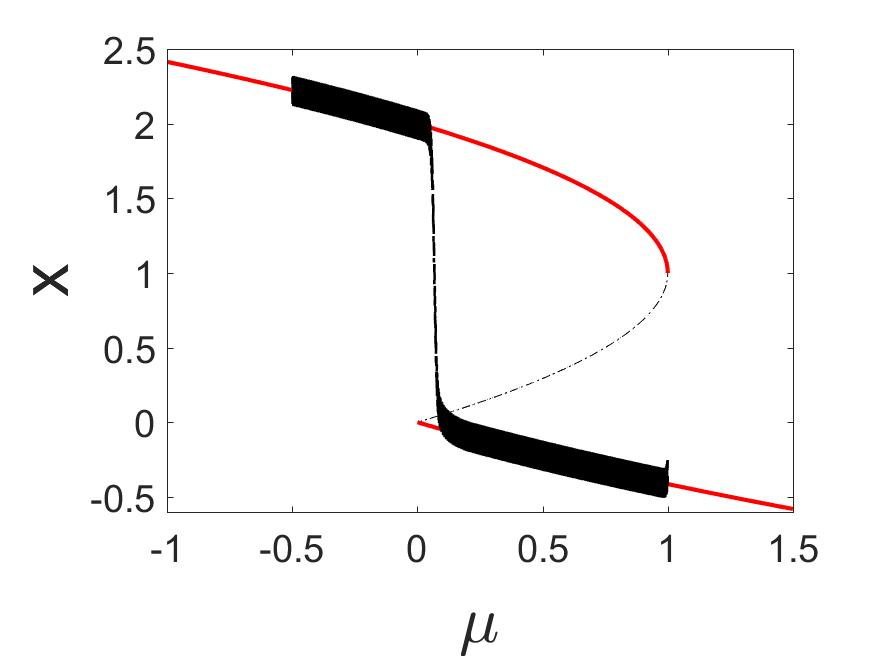
\includegraphics[width=\linewidth]{oneD/slowosc_bif_diagram_small.jpg}
 \caption{}
\end{subfigure}%
\begin{subfigure}{.5\textwidth}
 \centering
 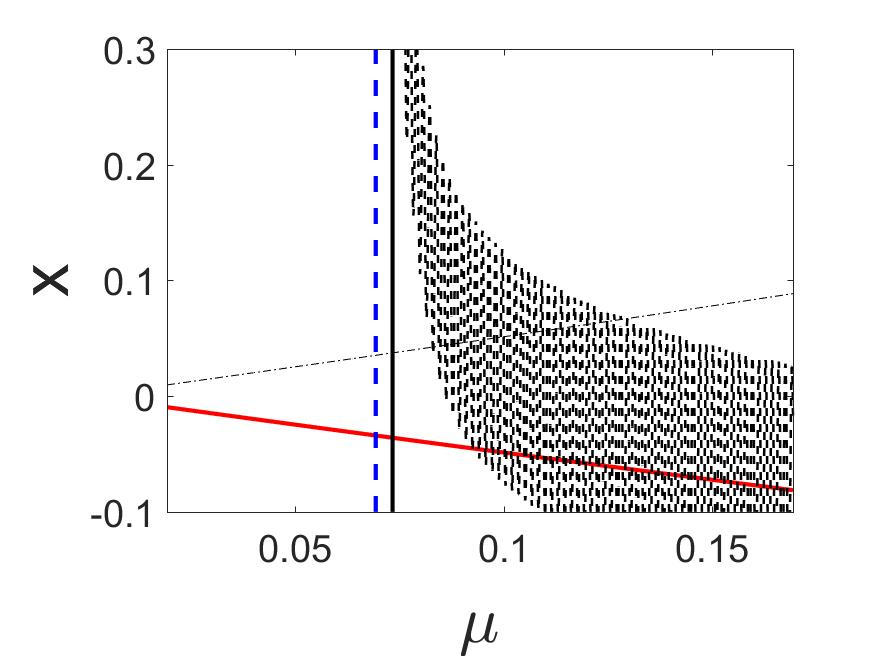
\includegraphics[width=\linewidth]{oneD/slowosc_bif_diagram_small_zoom.jpg}
 \caption{}
\end{subfigure}
\caption{Parameter values are $\epsilon=.05$, $\lambda=.8$ and $A=4$. On the left, this is the bifurcation diagram for the canonical system \eqref{eq:oneD_canonical} with the numerical solution (black dotted line). On the right, this is a zoom in. The dotted vertical line is the tipping point $\mu_{\text{mixed}}$ \eqref{eq:oneD_slowosc_uglymu} (blue). The vertical line (black) is the numerically obtained tipping for $x>.5$.}
\label{fig:oneD_slowosc_numerical_small}
\end{figure}

In figure~\ref{fig:oneD_slowosc_numerical_medium}, we see an example of $\lambda$ falling into Case II but is close enough to 1 that we see mixed behavior in the tipping. Here the slow variation is now dominant and the oscillations are only noticeable in the zoom in. But the green dotted line is the tipping point approximation \eqref{eq:oneD_slow_tipping} from \autoref{sec:oneD_slow} and $\mu_{\text{mixed}}$ is approximating the tipping point well.

\begin{figure}[H]
\centering
\begin{subfigure}{.5\textwidth}
 \centering
 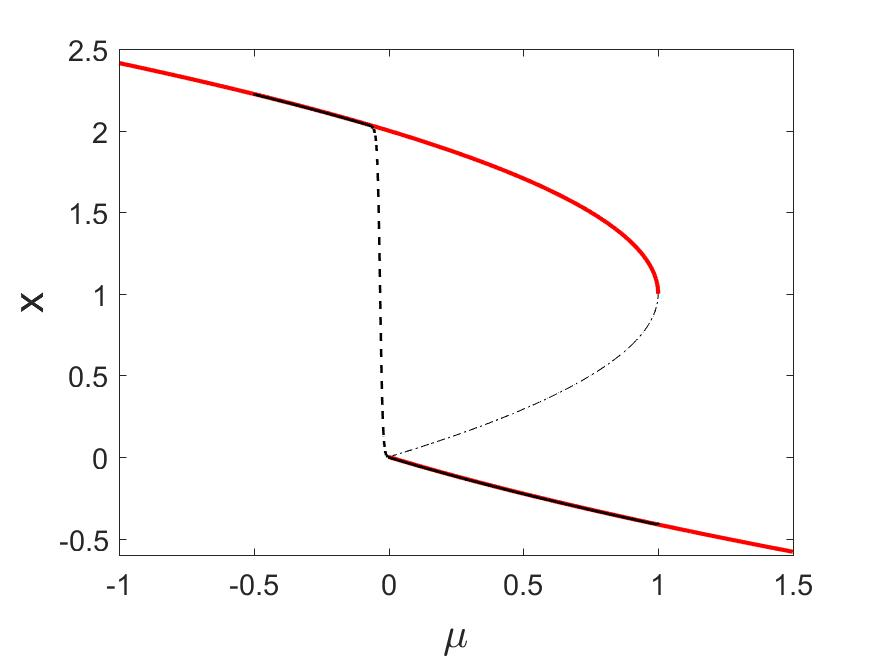
\includegraphics[width=\linewidth]{oneD/slowosc_bif_diagram_medium.jpg}
 \caption{}
\end{subfigure}%
\begin{subfigure}{.5\textwidth}
 \centering
 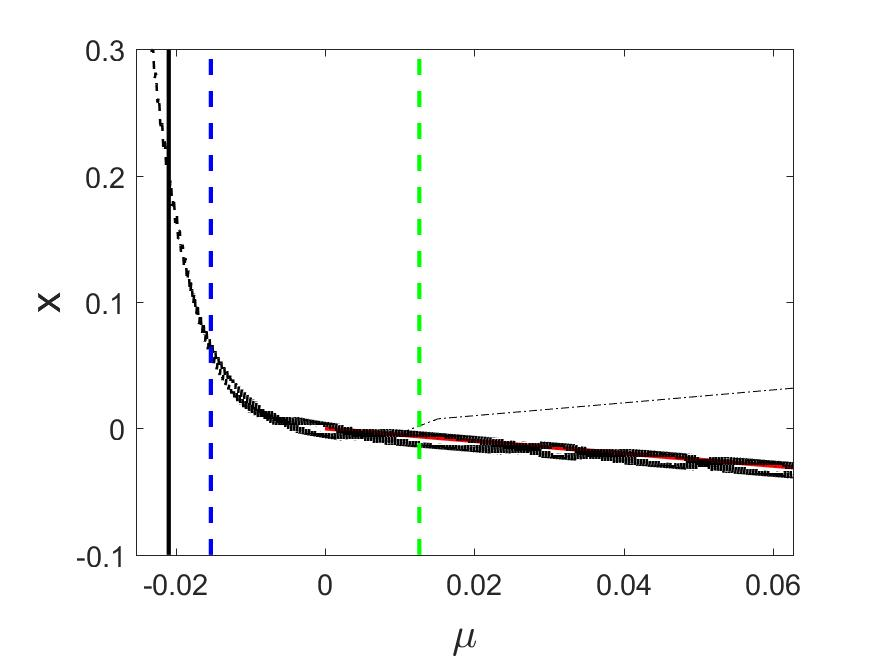
\includegraphics[width=\linewidth]{oneD/slowosc_bif_diagram_medium_zoom.jpg}
 \caption{}
\end{subfigure}
\caption{Parameter values are $\epsilon=.05$, $\lambda=1.05$ and $A=4$. On the left, this is the bifurcation diagram for the canonical system \eqref{eq:oneD_canonical} with the numerical solution (black dotted line). On the right, this is a zoom in. The dotted vertical lines are the tipping point $\mu_{\text{mixed}}$ \eqref{eq:oneD_slowosc_uglymu} (blue) and slowly varying tipping $\mu_{\text{slow}}$ \eqref{eq:oneD_slow_tipping} (green). The vertical line (black) is the numerically obtained tipping for $x>.5$.}
\label{fig:oneD_slowosc_numerical_medium}
\end{figure}

In figure~\ref{fig:oneD_slowosc_numerical_large}, we see an example of $\lambda$ falling into Case II but is far enough from 1 that we see almost entirely slow behavior in the tipping. Even upon closer inspection there it is hardly noticeable that oscillations are present in the model. The green dotted line is the tipping approximation \eqref{eq:oneD_slow_tipping} from \autoref{sec:oneD_slow}, and it is clear that this is a better approximation than the mixed tipping point.

\begin{figure}[H]
\centering
\begin{subfigure}{.5\textwidth}
 \centering
 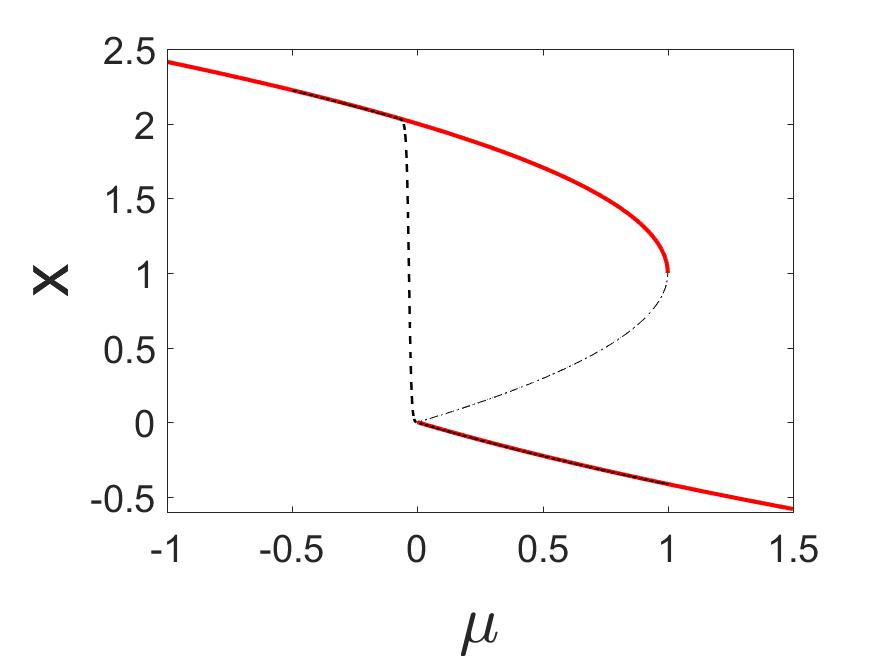
\includegraphics[width=\linewidth]{oneD/slowosc_bif_diagram_large.jpg}
 \caption{}
\end{subfigure}%
\begin{subfigure}{.5\textwidth}
 \centering
 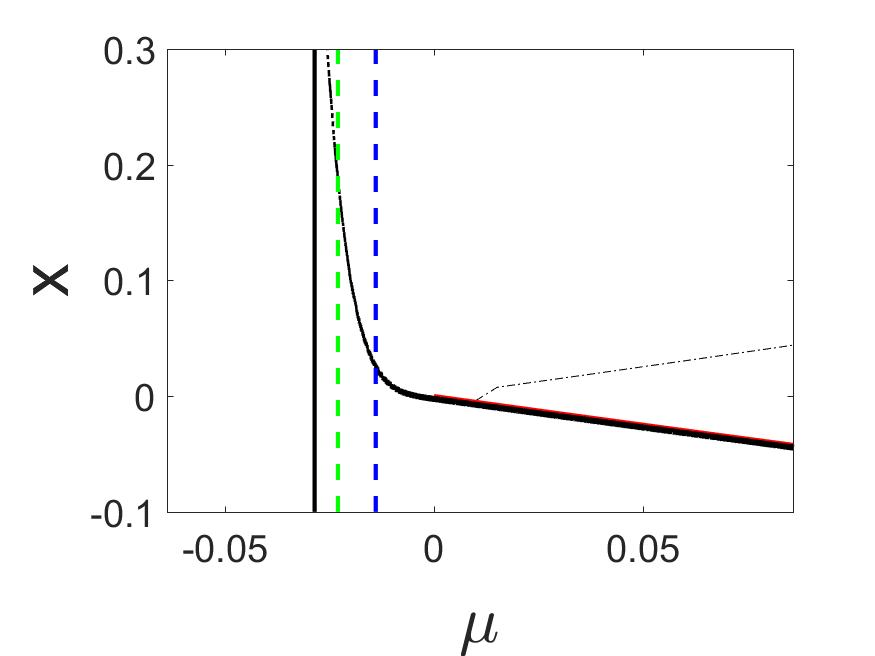
\includegraphics[width=\linewidth]{oneD/slowosc_bif_diagram_large_zoom.jpg}
 \caption{}
\end{subfigure}
\caption{Parameter values are $\epsilon=.05$, $\lambda=1.6$ and $A=4$. On the left, this is the bifurcation diagram for the canonical system \eqref{eq:oneD_canonical} with the numerical solution(black dotted line). On the right, this is a zoom in. The dotted vertical lines are the tipping point $\mu_{\text{mixed}}$ \eqref{eq:oneD_slowosc_uglymu} (blue) and slowly varying tipping $\mu_{\text{slow}}$ \eqref{eq:oneD_slow_tipping} (green). The vertical line (black) is the numerically obtained tipping for $x>.5$.}
\label{fig:oneD_slowosc_numerical_large}
\end{figure}

In figure~\ref{fig:oneD_slowosc_lambdacomp} we compare the tipping between Case I and Case II with the numerical tipping. For smaller $\lambda$, the frequency $\Omega$ gets smaller and the Case I tipping becomes more predominant. But for the analysis performed in this section, $\Omega\gg 1$ and for $\lambda\le\frac{1}{2}$ we have $\Omega\sim O(1)$. We do not consider low frequency corresponding to $\lambda\le\frac{1}{2}$ in this section. The larger $\lambda$ becomes, the less effect we see from the oscillatory forcing until it is negligible for some $\lambda>1$. This is also seen in the asymptotic solution for each case, \eqref{eq:oneD_slowosc_outersoln}, \eqref{eq:oneD_slowosc_caseIsoln}, and \eqref{eq:oneD_slowosc_caseIIsoln} where the oscillatory component of the term has a $\epsilon^\lambda$ coefficient and shrinks the effects as $\lambda$ grows.

\begin{figure}[H]
\centering
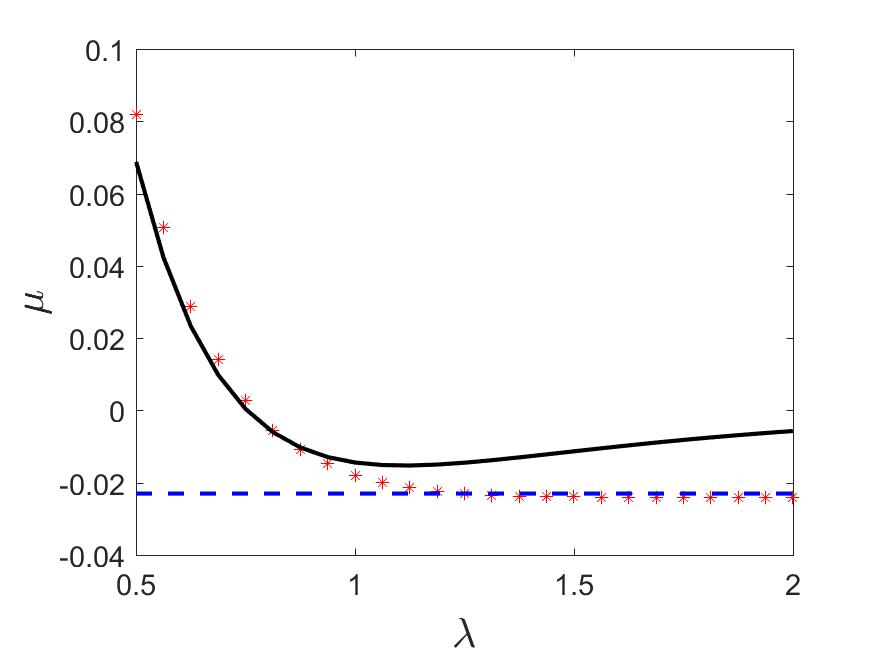
\includegraphics[width=0.7\textwidth]{oneD/slowosc_lambdacomp.jpg}
\caption{An example of numerical tipping (red stars) as the numerical solution to \eqref{eq:oneD_canonical} passes $x=.5$ for the last time. Parameter values are $\epsilon=.01$ and $A=4$. The lines are the Case I tipping estimate \eqref{eq:oneD_slowosc_uglymu} (black solid line) and the Case II tipping estimate \eqref{eq:oneD_slow_tipping} (blue dotted line).}
\label{fig:oneD_slowosc_lambdacomp}
\end{figure} 

The performance of our estimates are seen in figure~\ref{fig:oneD_slowosc_epscomp}. For Case I tipping, the range of appropriate $\epsilon$ is highly dependent on the choice in $\lambda$. Often, the range is very small to get accurate estimates. Both case approximations have good performance over a reasonable range of $\epsilon$.


\begin{figure}[H]
\centering
\begin{subfigure}{.5\textwidth}
 \centering
 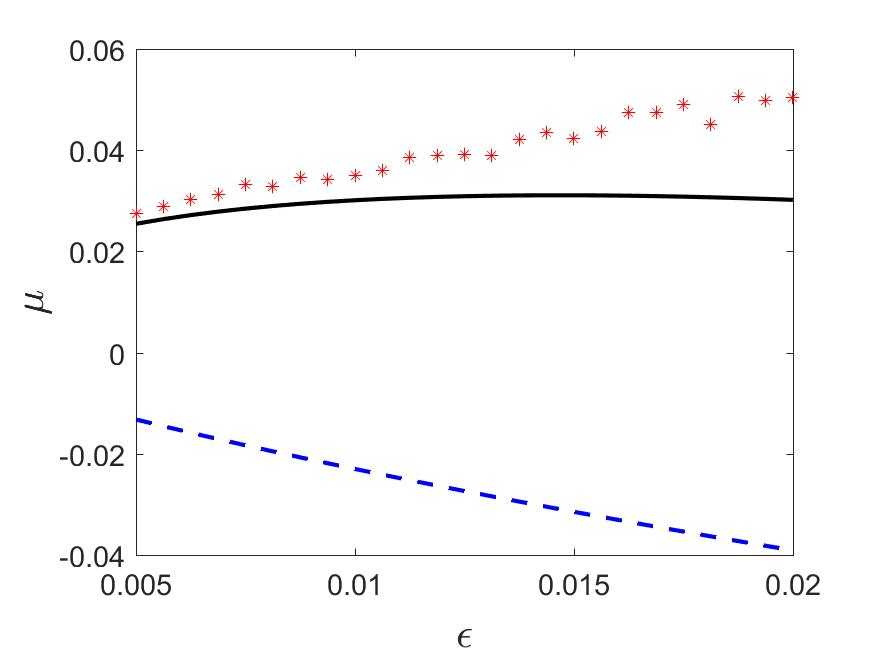
\includegraphics[width=\linewidth]{oneD/slowosc_epscomp_case2.jpg}
 \caption{$\lambda=.8$}
\end{subfigure}%
\begin{subfigure}{.5\textwidth}
 \centering
 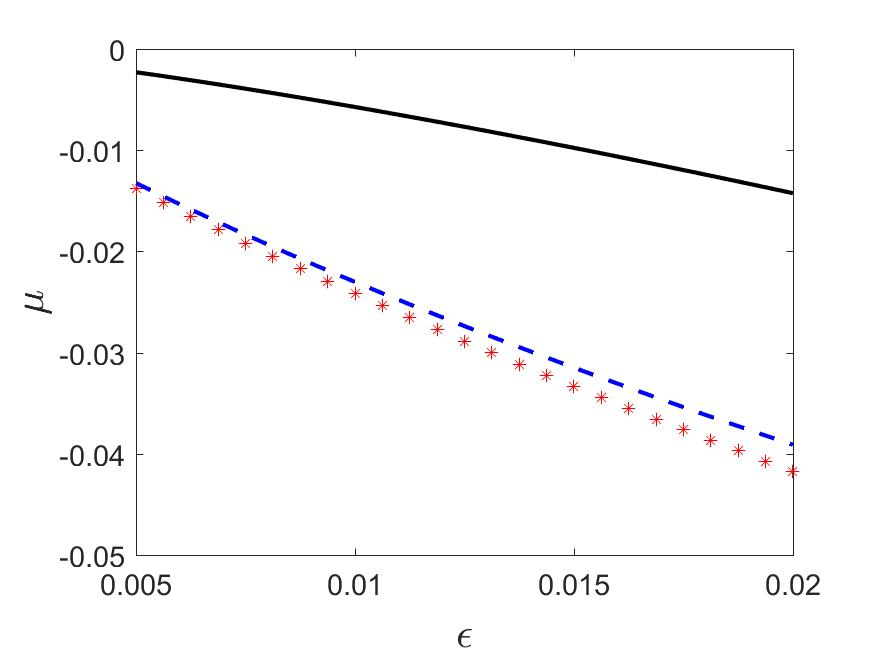
\includegraphics[width=\linewidth]{oneD/slowosc_epscomp_case3.jpg}
 \caption{$\lambda=1.3$}
\end{subfigure}
\caption{The numerical tipping (red stars) follows the appropriate case depending on $\lambda$. The Case I tipping estimate (black solid line) and the Case II tipping estimate (blue dotted line) are shown.}
\label{fig:oneD_slowosc_epscomp}
\end{figure}

\subsection{Stability}

Similarly to \autoref{sec:oneD_highfreqosc}, there are two ranges for $\lambda$ that govern the stability of solutions found in our analysis, $\lambda\le 1$ and $\lambda>1$.

\subsubsection{Case I: $\lambda\le 1$}

Recall for this case, we must have $\lambda\in (\frac{1}{2},1]$ and for this range, we found the inner equation

\begin{equation}\label{eq:oneD_slowosc_innerintegral}
{v_0}_t= -\epsilon^{1-\lambda}m(t)+\frac{1}{\pi}\int_0^{2\pi}| v_0(t)- A\cos(T)|\,dT=f(t,v_0).
\end{equation}

As in our analysis, we consider two regions of the solution $v_0(t)$ for this integral, in \autoref{subsec:oneD_slowosc_caseI} with Sub-Case I: $v_0(t)\le - |A|$ and in \autoref{subsec:oneD_slowosc_caseII} with Sub-Case II: $|v_0(t)|\le |A|$ where each these sub-cases deal with the respective size of $v_0(t)$ to the amplitude of the effective oscillations.

\subsubsection*{Sub-Case I: $v_0(t)\le - |A|$}

Recall from the analysis that the equation \eqref{eq:oneD_slowosc_innerintegral} simplifies in this region of $v_0(t)$ and has the following inner equation and pseudo-equilibrium $z^0(t)$

\begin{equation}\label{eq:oneD_slowosc_stabilitysubcaseI}
{v_0}_t= -\epsilon^{1-\lambda}m(t) -2v_0=f(t,v_0), \quad z^0(t)=-\epsilon^{1-\lambda}\frac{m(t)}{2}.
\end{equation}

As we saw in \autoref{sec:oneD_slow}, special treatment of the pseudo-equilibrium stability analysis is needed with linear perturbations $v_0(t)=z^0(t)+u(t)$ where $\lVert u(t)\rVert \ll 1$ and $z^0_t = -\epsilon^{1-\lambda}\frac{m_t}{2}=\frac{\epsilon^{1-\lambda}}{2}$. The resulting Taylor expansion is thus

\begin{equation*}
\begin{aligned}
{v_0}_t =& f(t,z^0)+f_{v_0}(t,v_0)(v_0(t)-z^0(t))+O(\lVert v_0(t)-z^0(t) \rVert^2),\\
u_t =&-\frac{\epsilon^{1-\lambda}}{2}-2u.
\end{aligned}
\end{equation*}

This leads to the conclusion that equation \eqref{eq:oneD_slowosc_stabilitysubcaseI} causes perturbations to decay exponentially to just below the pseudo-equilibrium. Hence we find the pseudo-equilibrium to be a hyperbolic and asymptotically attracting solution.

\subsubsection*{Sub-Case II: $v_0(t)\le |A|$}

With the Taylor approximation from the analysis \eqref{eq:oneD_slowosc_subcaseIItaylor}, we have the following inner equation and pseudo-equilibrium $z^0(t)$

\begin{equation}\label{eq:oneD_slowosc_stabilitysubcaseII}
{v_0}_t= -\epsilon^{1-\lambda}m(t) +\frac{4|A|}{\pi}+\frac{2}{\pi |A|}v_0^2=f(t,v_0),\quad z^0(t)=-C \sqrt{\epsilon^{1-\lambda}m(t)-\frac{4|A|}{\pi}}
\end{equation}

We consider simple linear perturbations to this pseudo-equilibrium \eqref{eq:oneD_slowosc_stabilitysubcaseII}, $v_0(t)=z^0(t)+u(t)$ with $\lVert u(t) \rVert \ll 1$. Treating the pseudo-equilibrium carefully, we find that the slowly varying component of the equilibrium contributes to the derivative. Thus we have

\begin{equation}
\begin{aligned}
{v_0}_t =& z^0_t(t) +u_t,\\
z^0_t(t) = & \begin{cases}
\frac{\epsilon^{1-\lambda}}{2C\sqrt{\epsilon^{1-\lambda}m(t)-\frac{4|A|}{\pi}}} & \epsilon^{1-\lambda}m(t)> \frac{4|A|}{\pi},\\
0 & \epsilon^{1-\lambda}m(t) =\frac{4|A|}{\pi}.
\end{cases}
\end{aligned}
\end{equation}

Now applying a Taylor expansion, we find the following behavior of perturbations

\begin{equation}\label{eq:oneD_slowosc_stabilitysubcaseIIeq}
\begin{aligned}
{v_0}_t =& f(t,z^0)+f_{v_0}(t,z^0)(v_0-z^0(t))+O(\lVert v_0(t)-z^0(t) \rVert),\\
u_t =&\begin{cases}
-\frac{\epsilon^{1-\lambda}}{2C\sqrt{\epsilon^{1-\lambda}m(t)-\frac{4|A|}{\pi}}}-2\sqrt{\epsilon^{1-\lambda}m(t)-\frac{4|A|}{\pi}} u & \epsilon^{1-\lambda}m(t)>\frac{4|A|}{\pi},\\
0 & \epsilon^{1-\lambda}m(t)=\frac{4|A|}{\pi}.
\end{cases}
\end{aligned}
\end{equation}

From \eqref{eq:oneD_slowosc_stabilitysubcaseIIeq}, we find that the perturbations decay to a fixed negative quantity. This indicates, much like \autoref{sec:oneD_slow}, that there is an attracting solution below the pseudo-equilibrium. The negative sign describes exponential decay and hence this equilibrium is hyperbolic and asymptotically stable for $\epsilon^{1-\lambda}m(t)>\frac{4|A|}{\pi}$ or $\mu(t)>\frac{4|A|}{\pi \Omega}$. But for $\epsilon^{1-\lambda}m(t)=\frac{4|A|}{\pi}$ or $\mu(t) =\mu_{\text{osc}}$, the stability of \eqref{eq:oneD_slowosc_stabilitysubcaseIIeq} suddenly becomes non-hyperbolic. This tells us that we lose stability at the oscillatory bifurcation but the tipping point occurs afterwards, which agrees with the conclusion in the tipping approximation from \eqref{eq:oneD_slowosc_caseItipping}.

\subsubsection{Case II: $\lambda>1$}

From the analysis, we discovered that for as long as $\epsilon^{\lambda-1}A\sim O(1)$, then we have very similar behavior in the tipping for this case. With the Taylor approximation from the analysis \eqref{eq:oneD_slowosc_caseII_integral}, the inner equation and pseudo-equilibrium $z^0(t)$ is

\begin{equation}\label{eq:oneD_slowosc_stabilitycaseII}
\begin{aligned}
y_0=&-m(t) +\epsilon^{\lambda-1}\frac{2|A|}{\pi}+\epsilon^{1-\lambda}\frac{2}{\pi |A|}y_0^2=f(t,y),\\
z^0(t)=&-\epsilon^{\lambda-1}C\sqrt{m(t)-\epsilon^{\lambda-1}\frac{4|A|}{\pi}}.
\end{aligned}
\end{equation}

Similarly to Case I, we consider simple linear perturbations to this pseudo-equilibrium \eqref{eq:oneD_slowosc_stabilitycaseII}, $y_0(t)=z^0(t)+u(t)$ with $\lVert u(t) \rVert \ll 1$. Treating the pseudo-equilibrium carefully, we find that the slowly varying component of the equilibrium contributes to the derivative. Thus we have

\begin{equation}
\begin{aligned}
{y_0}_t =& z^0_t(t) +u_t,\\
z^0_t(t) = & \begin{cases}
\frac{\epsilon^{\lambda-1}}{2C\sqrt{m(t)-\epsilon^{\lambda-1}\frac{4|A|}{\pi}}} & m(t)> \epsilon^{\lambda-1}\frac{4|A|}{\pi},\\
0 & m(t) =\epsilon^{\lambda-1}\frac{4|A|}{\pi}.
\end{cases}
\end{aligned}
\end{equation}

Now applying a Taylor expansion, we find the following behavior of perturbations

\begin{equation}\label{eq:oneD_slowosc_stabilitycaseIIeq}
\begin{aligned}
{y_0}_t =& f(t,z^0)+f_{y_0}(t,z^0)(y_0-z^0(t))+O(\lVert y_0-z^0(t) \rVert^2),\\
u_t =&\begin{cases}
-\frac{\epsilon^{\lambda-1}}{2C\sqrt{m(t)-\epsilon^{\lambda-1}\frac{4|A|}{\pi}}}-2\sqrt{m(t)-\epsilon^{\lambda-1}\frac{4|A|}{\pi}} u & m(t)>\epsilon^{\lambda-1}\frac{4|A|}{\pi},\\
0 & m(t)=\epsilon^{\lambda-1}\frac{4|A|}{\pi}.
\end{cases}
\end{aligned}
\end{equation}

But the conclusions from Case I still apply to \eqref{eq:oneD_slowosc_stabilitycaseIIeq} and thus we still have an attracting solution until $\mu(t)=\mu_{\text{osc}}$ and expect to see tipping occurring after the oscillatory bifurcation which is consistent with our tipping approximation for this case.

On the other hand, for large $\lambda$, the integral \eqref{eq:oneD_slowosc_caseII_integral} approaches

\begin{equation}\label{eq:oneD_slowosc_stabilitycaseII}
{y_0}_t=-m(t)+2|y_0|.
\end{equation}
But this is the same type of behavior from \autoref{sec:oneD_slow}, where we found that for $m(t)\ge 0$ our pseudo-equilibrium was attracting and for $m(t)<0$ that searching for the pseudo-equilibrium causes a contradiction. Thus, we conclude that the tipping point occurs in the region of $m(t)<0$ which agrees with \eqref{eq:oneD_slow_tipping}.


\chapter{Two Component Model}
\label{chap:twoD}
With the methods and approaches developed in \autoref{chap:oneD} for the one-dimensional model, we have an expectation of the behavior of the two-dimensional Stommel model around the non-smooth bifurcation under similar conditions. With the bifurcation structure we explored in \autoref{chap:introduction}, we consider a generalization of the Stommel model with

\begin{equation}\label{eq:twoD_canonical}
  \begin{aligned}
   \dot{V} & =  \eta_1-\eta_2+\eta_3(T-V)-T-V|V|+A\sin(\Omega t), \\
   \dot{T}     & =  \eta_1-T(1+|V|)+B\sin(\Omega t),  \\
  \dot{\eta_2}  & =  -\epsilon\\
  V(0)=&V^0,\quad T(0)=T^0, \quad \eta_2(0)={\eta_2}^0>\eta_1\eta_3,
  \end{aligned}
\end{equation}

with slow variation $\epsilon\ll 1$, high frequency $\Omega\gg 1$, amplitudes of oscillation $A$ and $B$, and model parameters $\eta_1$ and $\eta_3$ as positive constants. We assume the initial conditions $V^0$, $T^0$ and $\eta_2^0$ are along the lower equilibrium branch which puts emphasis on the non-smooth behavior of the Stommel model with two additional features. First, we allow for slow variation in the bifurcation parameter which has been shown to be realistic since the $\eta_2$ is related to the freshwater flux and therefore not a fixed parameter; the same assumption is made in Roberts \cite{roberts2017relaxation}. Second, we consider periodic forcing in the additive parameters $\eta_1$ and $\eta_2$ to account for oscillations in the observed behavior in Huybers \cite{huybers2005obliquity}. To fully understand the effects of each component on the model, we consider them individually before putting them together.

For the remainder of this paper, we make two assumptions: first that $\eta_3<1$ locates the smooth bifurcation of \eqref{eq:twoD_canonical}  in the positive $V$ region. The value of $\eta_3$ describes the relative strength of the temperature relaxation to that of salinity, and it is frequently assumed that salinity has a slower relaxation, giving $\eta_3<1$. We restrict our attention to $\eta_3<1$, since the case of $\eta_3>1$ follows similarly. The second assumption we make is that even though we have a model in terms of $V$ and $T$, the variable $V$ is driving the dynamics of the system as confirmed in the analysis below. This assumption means that we want to understand the non-smooth behavior in $V$ where $T$ follows in response to the effects of $V$. The evidence below shows changes in temperature respond to changes in salinity. This assumption allows for a reduced model, expressing the behavior of $T$ in terms of $V$ to find equations in only one variable.

\section{Slowly Varying Bifurcation Parameter}
\label{sec:twoD_slow}

We consider the slow variation mechanism to understand the effects on the Stommel model \eqref{eq:twoD_canonical} with $\epsilon>0$ and $A=B=0$, where the bifurcation parameter $\eta_2$ slowly varies without oscillatory forcing. Then we expect to find a tipping point in the neighborhood of the aforementioned non-smooth bifurcation at $\eta_2=\eta_1\eta_3$. With the choice of $\eta_3<1$, the lower branch with $V<0$ is the branch we focus on in order to approach the non-smooth behavior, thus \eqref{eq:twoD_canonical} is

\begin{equation}\label{eq:twoD_slow_negative}
 \begin{aligned}
   \dot{V} & =  \eta_1-\eta_2(t)+\eta_3(T-V)-T+V^2, \\
   \dot{T} & =  \eta_1-T(1-V),  \\
  \dot{\eta_2}  & =  -\epsilon.
  \end{aligned}
\end{equation}

From \autoref{sec:oneD_slow}, we learned that the one-dimensional model had a solution that displayed one type of behavior away from the non-smooth $x=0$ and another type close to $x=0$ and a local analysis gave insight into the tipping. Here we search for an outer solution to \eqref{eq:twoD_slow_negative} that helps us understand the behavior of system away from the non-smooth $V=0$.  Since we have slow variation in $\eta_2$, we choose to scale the system \eqref{eq:twoD_slow_negative} with the 'slow' time $\tau=\epsilon t$

\begin{equation}\label{eq:twoD_slow_slowsystem}
\begin{aligned}
\epsilon V_\tau =&\eta_1-\eta_2(\tau)+\eta_3(T-V)-T+V^2, \\
\epsilon T_\tau & =  \eta_1-T(1-V),  \\
  {\eta_2}_\tau  & =  -1.
\end{aligned}
\end{equation}

We use asymptotic expansions in terms of the small quantity $\epsilon$ to look for slowly varying solutions. Here we choose

\begin{equation}\label{eq:twoD_slow_outerexpansion}
\begin{aligned}
V(\tau)\sim &V_0(\tau)+\epsilon V_1(\tau)+\epsilon^2 V_2(\tau)+\ldots\\
T(\tau)\sim & T_0(\tau)+\epsilon T_1(\tau)+\epsilon^2 T_2(\tau)+\ldots
\end{aligned}
\end{equation}

and substitute \eqref{eq:twoD_slow_outerexpansion} into \eqref{eq:twoD_slow_slowsystem} to find

\begin{equation*}
\begin{aligned}
 \epsilon{V_0}_\tau+\epsilon^2{V_1}_\tau+\ldots =&\begin{aligned}[t]
\eta_1-&\eta_2(\tau)+\eta_3(T_0-V_0)-T_0+V_0^2\\
&+\epsilon(\eta_3(T_1-V_1)-T_1-2V_1V_0)+\ldots
\end{aligned}\\
\epsilon{T_0}_\tau+\epsilon^2{T_1}_\tau+\ldots=&\eta_1-T_0(1-V_0)+\epsilon(-T_1(1-V_0)+V_1T_0)+\ldots
\end{aligned}
\end{equation*}

Here we separate at each order of $\epsilon$ to find the following system of equations

\begin{align}
\label{eq:twoD_slow_outerO1}
O(1):\quad & \begin{cases}
	0 =& \eta_1-\eta_2(\tau)+\eta_3(T_0-V_0)-T_0+V_0^2 , \\
	0 =&  \eta_1-T_0(1-V_0),\\
\end{cases}\\
\label{eq:twoD_slow_outerO2}
O(\epsilon):\quad & \begin{cases}
	{V_0}_\tau = & \eta_3(T_1-V_1)-T_1+2V_1V_0,\\
	{T_0}_\tau =&  -T_1(1-V_0)+V_1T_0,
\end{cases}
\end{align}

We then solve \eqref{eq:twoD_slow_outerO1} simultaneously for the pseudo-equilibria noting that $T_0$ is explicitly in terms of $V_0$ 

\begin{equation}\label{eq:twoD_slow_equilibria}
\begin{aligned}
T_0(V_0)=&\frac{\eta_1}{1-V_0},\\
0=\eta_1-\eta_2(\tau)-T_0(V_0)&+\eta_3(T_0(V_0)-V_0)+V_0^2.
\end{aligned}
\end{equation}

With $T_0$ and $V_0$ found, we solve \eqref{eq:twoD_slow_outerO2} for $T_1$ explicitly in terms of $V_1$ 

\begin{equation}\label{eq:twoD_slow_equilcorrec}
\begin{aligned}
&T_1(V_1) = \frac{{T_0}_\tau-T_0(V_0)V_1}{1-V_0},\\
V_1 =& \frac{-(1-V_0){V_0}_\tau+(1-\eta_3){T_0}_\tau({V_0}_\tau)}{(1-\eta_3)T_0(V_0)+(\eta_3-2V_0)(1-V_0)}.
\end{aligned}
\end{equation}

This gives the first few terms of the asymptotic expansion \eqref{eq:twoD_slow_outerexpansion} with \eqref{eq:twoD_slow_equilibria} and \eqref{eq:twoD_slow_equilcorrec}. Given these expressions, it is not immediately obvious in the two-dimensional problem when the outer solution breaks down. However, noting that for $V_0\to 0$ the asymptotic expansion for $V$ is no longer valid, we rescale the system to find an inner equation in this region. 

Analogous to \autoref{sec:oneD_slow}, this corresponds to the non-smooth bifurcation at $\eta_2=\eta_1\eta_3$ when $V=0$ and $T=\eta_1$, so it makes the most sense to rescale \eqref{eq:twoD_canonical} around these values. This results in the rescaled variables

\begin{equation}\label{eq:twoD_slow_rescale}
\begin{aligned}
\eta_2=&\eta_1\eta_3+\epsilon n,\\
V=&\epsilon X,\\
T=&\eta_1+\epsilon Y.
\end{aligned}
\end{equation}

Then we introduce these local variables \eqref{eq:twoD_slow_rescale} into the canonical system \eqref{eq:twoD_canonical} to find the following inner system

\begin{equation}\label{eq:twoD_slow_inner}
\begin{aligned}
   \dot{X} & =  -n(t)-\eta_3 X-(1-\eta_3)Y-\epsilon X|X|, \\
   \dot{Y} & =  -\eta_1 |X|-Y-\epsilon |X|Y,  \\
  \dot{n}  & =  -1.
  \end{aligned}
\end{equation}

We outline the influence of the parameters $\eta_1$ and $\eta_3$ on the behavior of a solution. We already determined from the introduction that $\eta_3$ determines the orientation of the problem, but here we find a relationship between the parameters $\eta_1$ and $\eta_3$ by viewing \eqref{eq:twoD_slow_inner} as a $2\times 2$ system of spatial coordinates and linearizing. This results in 

\begin{equation}\label{eq:twoD_slow_innermatrix}
\begin{pmatrix}
\dot{X}\\
\dot{Y}
\end{pmatrix}=
\begin{pmatrix}
-\eta_3 & -(1-\eta_3) \\ 
-\eta_1\text{sgn}(X) & -1
\end{pmatrix}
\begin{pmatrix}
X\\
Y
\end{pmatrix}-
\begin{pmatrix}
n(t)\\
0
\end{pmatrix}.
\end{equation}

Here a linearized stability analysis about the pseudo-equilibria similar to \cite{seydel2009practical} is needed to determine the stability of the lower pseudo-equilibria. This is performed in Dijkstra \cite{dijkstra2013nonlinear} and hence we note that both stability of the lower branch and non-hyperbolic behavior at $({\eta_2}_{ns},V_{ns})=(\eta_1\eta_3,0)$ is observed. Thus we expect our tipping point to occur just after the standard non-smooth bifurcation. With this in mind, we consider $V>0$ and with \eqref{eq:twoD_slow_innermatrix} we find the inner system

\begin{equation}\label{eq:twoD_slow_positiveinner}
 \begin{aligned}
   \dot{X} & =  -n(t)-\eta_3 X-(1-\eta_3)Y-\epsilon X^2, \\
   \dot{Y} & =  -\eta_1 X-Y-\epsilon XY,  \\
  \dot{n}  & =  -1.
  \end{aligned}
\end{equation}

Following the approach from \autoref{sec:oneD_slow}, we change the differentiation to be in terms of $n$ to find

\begin{equation*}
\begin{pmatrix}
X_n\\
Y_n
\end{pmatrix}=
\begin{pmatrix}
\eta_3 & 1-\eta_3 \\ 
\eta_1 & 1
\end{pmatrix}
\begin{pmatrix}
X\\
Y
\end{pmatrix} +
\begin{pmatrix}
n+\epsilon X^2\\
\epsilon XY
\end{pmatrix}.
\end{equation*}

Seeking a leading order solution in this region, we drop the $\epsilon$ order terms to give 

\begin{equation}\label{eq:twoD_slow_uppermatrix}
\begin{pmatrix}
X_n\\
Y_n
\end{pmatrix}=
\begin{pmatrix}
\eta_3 & 1-\eta_3 \\ 
\eta_1 & 1
\end{pmatrix}
\begin{pmatrix}
X\\
Y
\end{pmatrix} +
\begin{pmatrix}
n\\
0
\end{pmatrix}.
\end{equation}

For the system \eqref{eq:twoD_slow_uppermatrix}, we find the following eigenvalues using \eqref{eq:twoD_slow_eigen}

\begin{equation}\label{eq:twoD_slow_uppereigen}
\lambda_{1,2}=\frac{\eta_3+1}{2}\pm\frac{1}{2}\sqrt{(1+\eta_3)^2+4(\eta_1(1-\eta_3)-\eta_3)}.
\end{equation}

These eigenvalues in \eqref{eq:twoD_slow_uppereigen} must be real as $\eta_3<1$ guarantees the discriminant is always positive. But the stability also follows as one of the eigenvalues is positive and the other is negative. This causes the solution to be unstable, which confirms tipping to occur in the region $V>0$. With real eigenvalues, the solution in the $V>0$ region takes the following exponential form with constants $K_{i,j}$ being component $j$ of the corresponding $i$ eigenvector 

\begin{equation}\label{eq:twoD_slow_innersoln}
\begin{aligned}
X(n)\sim& K_{1,1}e^{\lambda_1 n}+K_{2,1}e^{\lambda_2 n}+C_1 n+C_2,\\
Y(n)\sim& K_{1,2}e^{\lambda_1 n}+K_{2,2}e^{\lambda_2 n}+C_3 n+C_4.\\
\end{aligned}
\end{equation}

Translating both solutions in \eqref{eq:twoD_slow_inner} back to our original coordinates we find

\begin{equation}\label{eq:twoD_slow_inneroriginal}
\begin{aligned}
V(t)\sim&  \epsilon K_{1,1}e^{\lambda_1(\eta_2(t)-\eta_1\eta_3)/\epsilon}+\epsilon K_{2,1}e^{\lambda_1(\eta_2(t)-\eta_1\eta_3)/\epsilon}+O(\epsilon),\\
T(t)\sim& \eta_1+ \epsilon K_{1,2}e^{\lambda_1 (\eta_2(t)-\eta_1\eta_3)/\epsilon}+\epsilon K_{2,2}e^{\lambda_2 (\eta_2(t)-\eta_1\eta_3)/\epsilon}+O(\epsilon).
\end{aligned}
\end{equation}

With \eqref{eq:twoD_slow_inneroriginal} admitting the solution in the region $V>0$, we determine the system to tip once one of these exponentials becomes large (i.e $O(1/\epsilon)$), which causes the system to diverge away from our lower branch towards the upper stable branch. Thus the tipping point ${\eta_2}_{\text{slow}}$ is

\begin{equation}\label{eq:twoD_slow_tipping}
{\eta_2}_{\text{slow}}= \min\limits_i\{\eta_1\eta_3-\epsilon\ln\epsilon/\lambda_i\},\quad i=1,2.
\end{equation}

Thus we have the tipping for this problem with \eqref{eq:twoD_slow_tipping} and this has a similar form to the tipping point from \autoref{sec:oneD_slow}. As we found from \eqref{eq:twoD_slow_uppereigen}, one of the eigenvalues is always positive and it is with this we find that the tipping point is less than the bifurcation. This means the slow variation causes a delay in the rapid transition from the lower branch to the upper branch and the solution spends more time around the lower branch. These effects shrink as $\epsilon\to 0$ until we return to the static problem with $\epsilon=0$,

\begin{figure}[H]
\centering
\begin{subfigure}{.5\textwidth}
  \centering
  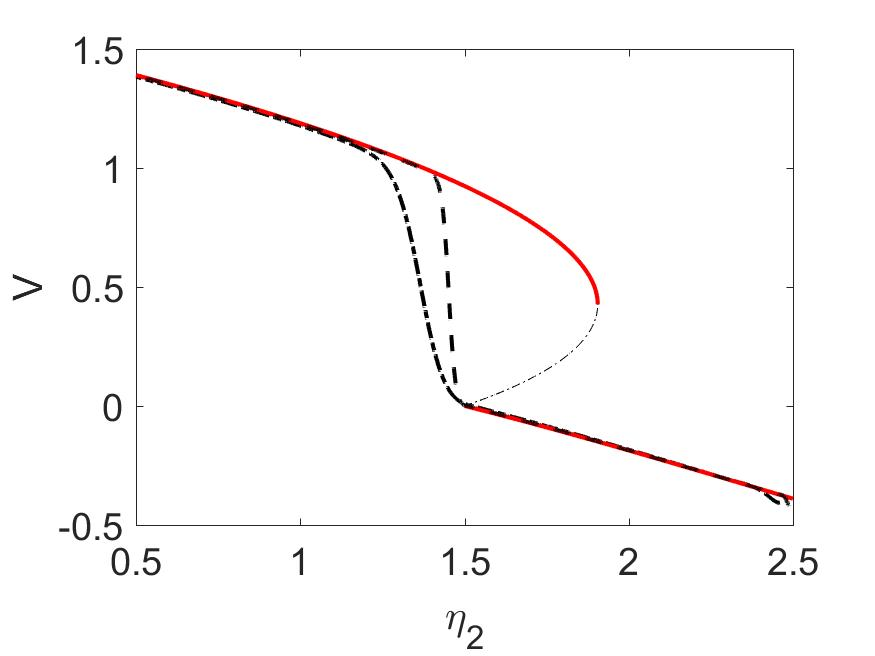
\includegraphics[width=\linewidth]{twoD/slow_bif_diagram.jpg}
  \caption{}
\end{subfigure}%
\begin{subfigure}{.5\textwidth}
  \centering
  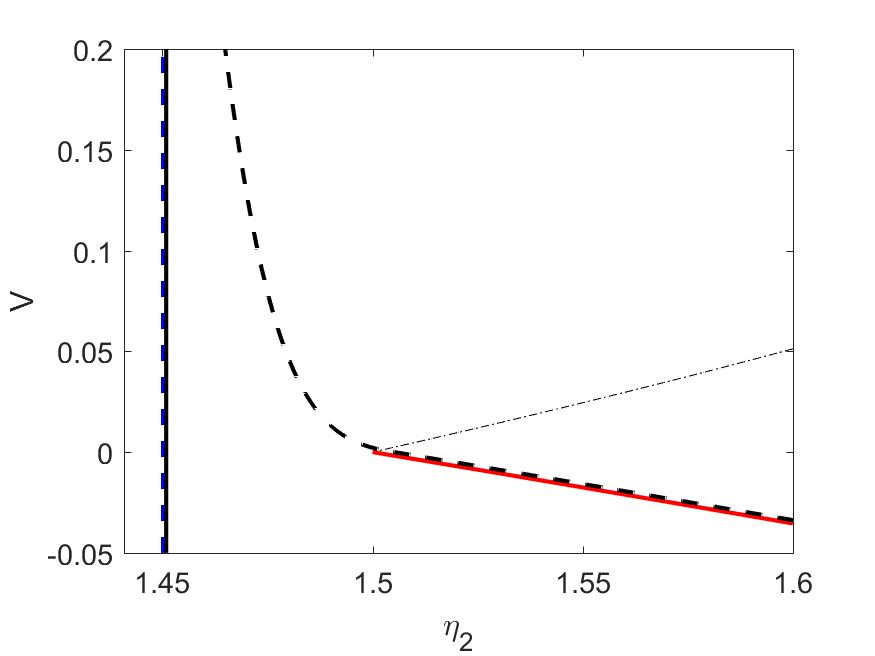
\includegraphics[width=\linewidth]{twoD/slow_bif_diagram_zoom.jpg}
  \caption{}
\end{subfigure}
\caption{In (a) the numerical solution (black dotted line) to \eqref{eq:twoD_canonical} is given with $\eta_1=4$, $\eta_3=.375$, and $\epsilon=.01$. In (b) a zoom in closer to the non-smooth bifurcation region where the blue dotted vertical line is the prediction \eqref{eq:twoD_slow_tipping} against the black solid vertical line which is the numerical tipping point.}
\label{fig:twoD_slow_Vnumerics}
\end{figure}

In figure~\ref{fig:twoD_slow_Vnumerics} an example of a slowly varying $\eta_2$ is given for a choice of $\epsilon$ in (a) and we zoom in around the non-smooth bifurcation in (b). Here we use the tipping criteria to be whenever $V>0.5$, this is large enough that the solution is strongly moving towards the upper branch and is around the point of the smooth bifurcation. The delay in moving towards the upper branch in the $V$ solution causes a similar delay in $T$ seen in figure~\ref{fig:twoD_slow_Tnumerics}. This is best explained in the perturbation equation \eqref{eq:twoD_slow_pertub} where the solution is attracted to below the pseudo-equilibrium. Thus when the tipping point in $V$ is reached, the solution for $T$ has yet to reach the maximum value. Here notice that after the tipping occurs, the numerical solution passes entirely over the unstable branch and even some of the upper stable branch before following the upper branch closely.

\begin{figure}[H]
\centering
\begin{subfigure}{.5\textwidth}
  \centering
  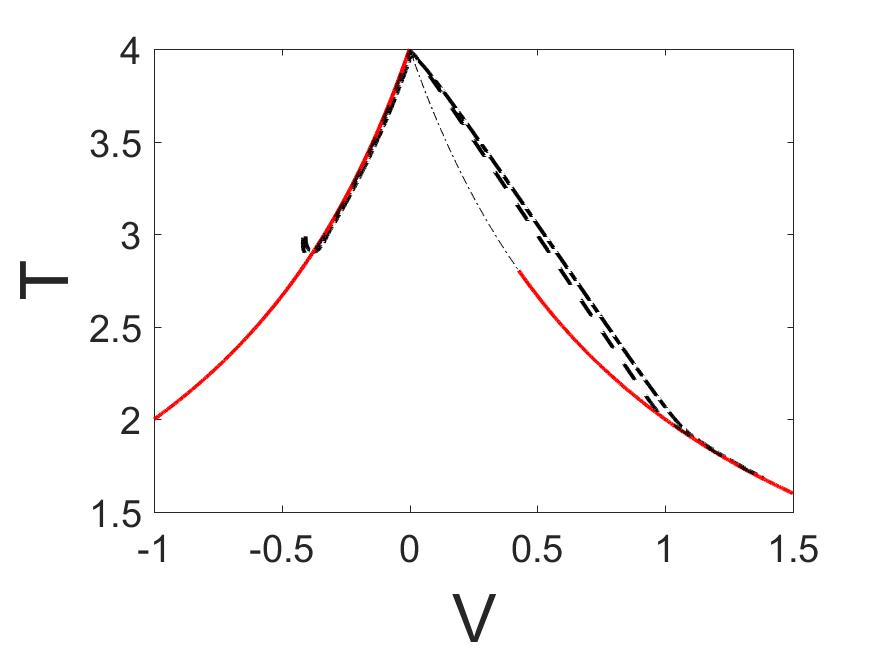
\includegraphics[width=\linewidth]{twoD/slow_bif_Tplot.jpg}
  \caption{}
\end{subfigure}%
\begin{subfigure}{.5\textwidth}
  \centering
  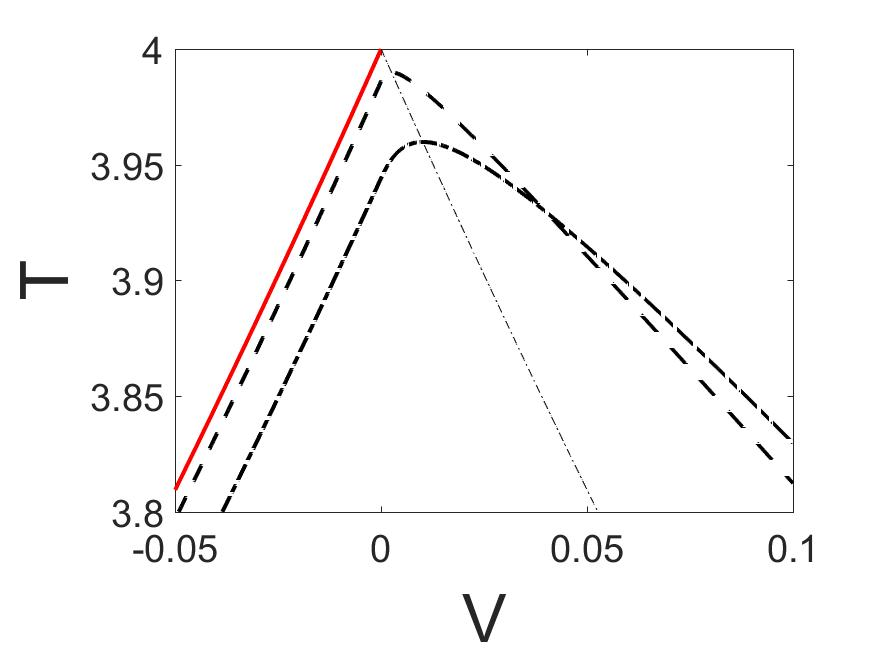
\includegraphics[width=\linewidth]{twoD/slow_bif_Tplot_zoom.jpg}
  \caption{}
\end{subfigure}
\caption{In (a) we have the numerical solution (black dotted) over the standard equilibrium plot for $V$ vs. $T$. In (b) a zoom of the bifurcation area.}
\label{fig:twoD_slow_Tnumerics}
\end{figure}

In figure~\ref{fig:twoD_slow_epscomp} we compare the numerical tipping to the predicted tipping in \eqref{eq:twoD_slow_tipping} over a range of $\epsilon$. Here we see performance even better than in section \autoref{sec:oneD_slow} as even for relatively large $\epsilon$ the prediction has small error. This is an artifact of having a higher dimensional problem, where now two exponentials in \eqref{eq:twoD_slow_inneroriginal} are dominating the behavior of the solution in the $V>0$ region. As in \autoref{sec:oneD_slow}, the concavity of the predicted tipping against the numerical tipping match very well and we can expect the prediction to hold for reasonably small values of $\epsilon$.

\begin{figure}[H]
\centering
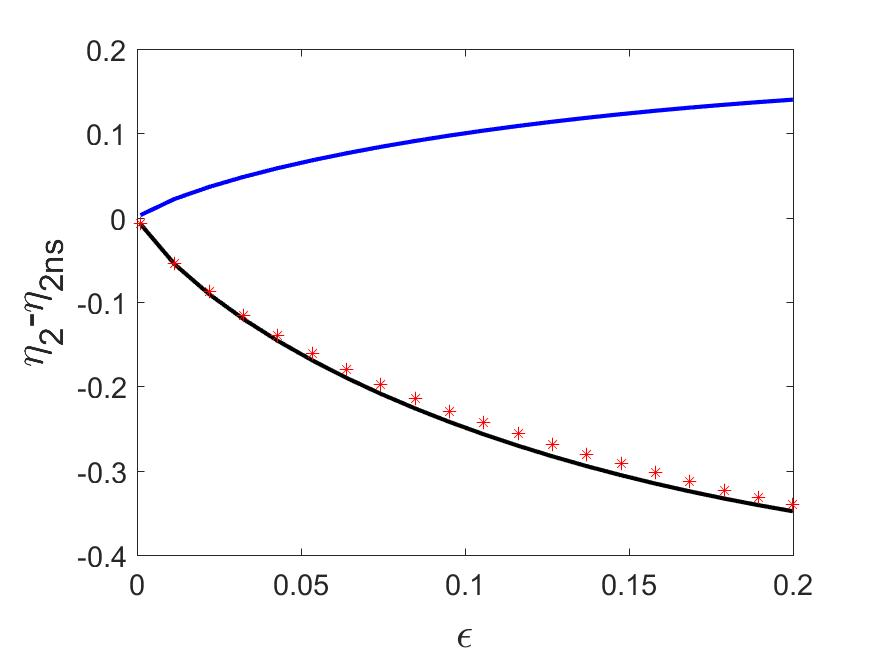
\includegraphics[width=\linewidth]{twoD/slow_epscomp.jpg}
\caption{The numerical tipping vs the estimate with $\eta_1=4$ and $\eta_3=\frac{3}{8}$, where ${\eta_2}_{\text{ns}}=\eta_1\eta_3$. The top blue line is the tipping of the second eigenvalue. The tipping criteria is $V>.5$.}
\label{fig:twoD_slow_epscomp}
\end{figure}

\section{High Frequency Oscillatory Forcing}
\label{sec:twoD_highfreqosc}

We consider oscillations occurring in the dynamics that is not originally encompassed by the Stommel model \cite{alley2003abrupt,huybers2005obliquity,marotzke2000abrupt,rahmstorf2000thermohaline,rahmstorf2002ocean,stastna2007box}. We choose to allow $\eta_1$ and $\eta_2$ to exhibit oscillatory behavior to account for this. As these parameters appear in both equations for $V$ and $T$, here we consider the canonical system \eqref{eq:twoD_canonical} with $A,B\sim O(1)$, $\Omega\gg 1$ and $\epsilon=0$ which is the purely oscillatory forcing problem. Under these conditions, like in the one-dimensional model in \autoref{sec:oneD_highfreqosc}, we expect to find oscillations that are attracting; this stable behavior should act like oscillations about the equilibria of a reduced inner problem. Thus our analysis must locate these equilibria as a function of $\eta_2$ in order to find the bifurcation.

To begin our analysis, we note that the dynamics occur on multiple time scales, a 'slow' $t$ and 'fast' $R = \Omega t$. Following the multiple scales method, we consider $V(t)=V(t,R)$ and $T(t)=T(t,R)$ and substituting this into \eqref{eq:twoD_canonical}, we get the system

\begin{equation}\label{eq:twoD_osc_multiscaleouter}
\begin{aligned}
V_R+\Omega^{-1}V_t = & \Omega^{-1}\left(\eta_1-\eta_2+\eta_3(T-V)-T-V|V|+A\sin(R)\right),\\
T_R+\Omega^{-1}T_t = & \Omega^{-1}\left(\eta_1-T(1+|V|)+B\sin(R)\right).
\end{aligned}
\end{equation}

We follow the lower branch to study dynamics near the non-smooth bifurcation. Thus we consider the system \eqref{eq:twoD_osc_multiscaleouter} with $V<0$

\begin{equation}\label{eq:twoD_osc_multiscaleouterlower}
\begin{aligned}
V_R+\Omega^{-1}V_t = & \Omega^{-1}\left(\eta_1-\eta_2+\eta_3(T-V)-T+V^2+A\sin(R)\right),\\
T_R+\Omega^{-1}T_t = & \Omega^{-1}\left(\eta_1-T(1-V)+B\sin(R)\right).
\end{aligned}
\end{equation}

From \eqref{eq:twoD_osc_multiscaleouterlower}, it makes sense to consider an asymptotic expansion for both $V$ and $T$ in terms of the small quantity that appears, $\Omega^{-1}$, with

\begin{equation}\label{eq:twoD_osc_outerexpansion}
\begin{aligned}
V(t,R)\sim V_0(t,R) +\Omega^{-1}V_1(t,R) +\Omega^{-2}V_2(t,R)+O(\Omega^{-3}),\\
T(t,R)\sim T_0(t,R) +\Omega^{-1}T_1(t,R) +\Omega^{-2}T_2(t,R)+O(\Omega^{-3}).
\end{aligned}
\end{equation}

Substituting \eqref{eq:twoD_osc_outerexpansion} into the system \eqref{eq:twoD_osc_multiscaleouterlower} gives

\begin{equation*}
\begin{aligned}
{V_0}_R+\Omega^{-1}{V_0}_t+\Omega^{-1}{V_1}_R+\ldots=&\begin{aligned}[t]\Omega^{-1}&(\eta_1-\eta_2+\eta_3(T_0-V_0)-T_0+V_0^2+A\sin(R))\\
+&\Omega^{-2}(\eta_3(T_1-V_1)-T_1+2V_1V_0)+\ldots
\end{aligned}\\
{T_0}_R+\Omega^{-1}{T_0}_t+\Omega^{-1}{T_1}_R+\ldots=&\begin{aligned}[t]  \Omega^{-1}&(\eta_1-T_0(1-V_0)+B\sin(R))\\
+&\Omega^{-2}(-T_1(1-V_0)+T_0V_1)+\ldots
\end{aligned}
\end{aligned}
\end{equation*}

Here we find the following equations separated by order of $\Omega^{-1}$ with

\begin{align}
\label{eq:twoD_osc_outerO1}
O(1):\quad & \begin{cases}
	{V_0}_R =&  0, \\
	{T_0}_R =&  0,\\
\end{cases}\\
\label{eq:twoD_osc_outerO2}
O(\Omega^{-1}):\quad & \begin{cases}
	{V_1}_R+{V_0}_t = & \eta_1-\eta_2+\eta_3(T_0-V_0)-T_0+V_0^2+A\sin(R),\\
	 {T_1}_R +{T_0}_t =&  \eta_1-T_0(1-V_0)+B\sin(R),
\end{cases}\\
\label{eq:twoD_osc_outerO3}
O(\Omega^{-2}):\quad & \begin{cases}
	{V_2}_R+{V_1}_t = & \eta_3(T_1-V_1)-T_1+2V_0V_1,\\
	 {T_2}_R +{T_1}_t =&  -T_1(1-V_0)+T_0V_1.
\end{cases}
\end{align}

We learn from \eqref{eq:twoD_osc_outerO1} that both our leading order terms are purely dependent on the slow variable, $V_0=V_0(t)$, $T_0=T_0(t)$. But much like \autoref{sec:oneD_highfreqosc}, we must introduce a solvability condition on the resonant terms to be able to solve for the correction terms, ensuring for the sub-linear growth resulting in a stable solution. Here, we use the Fredholm alternative \eqref{eq:Fredholm} on \eqref{eq:twoD_osc_outerO2}-\eqref{eq:twoD_osc_outerO3} and search for the equilibrium solutions, this is shown in \autoref{app:twoD}. This leads to the outer solution in original coordinates

\begin{equation}\label{eq:twoD_osc_outersoln}
\begin{aligned}
V\sim& V_0-\Omega^{-1} A\cos(\Omega t)+\dots\\
%\Omega^{-2}\left(V_2(t)+\left(A(\eta_3-2V_0)+B(1-\eta_3)\right)\sin(\Omega t)\right),\\
T\sim& T_0-\Omega^{-1} B\cos(\Omega t)+\ldots%\Omega^{-2}\left(T_2(t)+(1-V_0)B-T_0A)\sin(\Omega t)\right).
\end{aligned}
\end{equation}

Here both $V_0$ and $T_0$ are the same equilibrium solutions from the static model in the introduction with

\begin{equation*} \label{eq:twoD_lowerleadingorder}
\begin{aligned}
T_0(V_0)=&\frac{\eta_1}{1-V_0},\\
0=\eta_1-\eta_2+\eta_3&(T_0(V_0)-V_0)-T_0(V_0)+V_0^2.
\end{aligned}
\end{equation*}

For the one-dimensional model in \autoref{sec:oneD_highfreqosc}, we had to use a local expansion so we needed to scale both the coordinate $x$ as well as the parameter $\mu$ and analyze the local behavior around the axis $x=0$. Since we again have non-smooth dynamics at the axis $V=0$, we expect to use a local expansion for the two-dimensional model as well. While the precise scaling of the breakdown of the outer solution \eqref{eq:twoD_osc_outersoln} is too complex for us to search for, we instead observe that once $V_0$ becomes small the oscillations begin to dominate the solution and this is not consisten with our assumptions of the expansion. So we introduce a rescaling analogous to  \autoref{sec:oneD_highfreqosc}

\begin{equation}\label{eq:twoD_osc_scales}
\begin{aligned}
V=&\Omega^{-1}X,\\
T=& \eta_1 +\Omega^{-1}Y,\\
\eta_2=&\eta_1\eta_3+\Omega^{-1} n.
\end{aligned}
\end{equation}

Substituting \eqref{eq:twoD_osc_scales} into \eqref{eq:twoD_canonical} leads to the following inner system

\begin{equation}\label{eq:twoD_osc_innersystem}
\begin{aligned}
\dot{X}=& -n+\eta_3(Y-X)-Y-\Omega^{-1}X|X| +\Omega A\sin(\Omega t),\\
\dot{Y}=& -\eta_1|X|-Y -\Omega^{-1}|X|Y +\Omega A \sin(\Omega t).
\end{aligned}
\end{equation}

The form suggests behavior on the same time scales in \eqref{eq:twoD_osc_innersystem}, the 'slow' $t$ and the 'fast' $R=\Omega t$. Considering $X(t)=X(t,R)$ and $Y(t)=Y(t,R)$ gives the multiple scales inner system

\begin{equation}\label{eq:twoD_osc_innermulti}
\begin{aligned}
X_R+\Omega^{-1}X_t =& \Omega^{-1}\left(-n +\eta_3(Y-X)-Y\right)-\Omega^{-2}X|X|+A\sin(R),\\
Y_R+\Omega^{-1}Y_t =& \Omega^{-1}\left(-\eta_1|X|-Y\right)-\Omega^{-2}|X|Y+ B\sin(R).
\end{aligned}
\end{equation}

Once more, as we see the small quantity $\Omega^{-1}$ appearing in \eqref{eq:twoD_osc_innermulti}, we choose an expansion of the form

\begin{equation}\label{eq:twoD_osc_innerexpan}
\begin{aligned}
X(t,R)\sim& X_0(t,R)+\Omega^{-1}X_1(t,R)+O(\Omega^{-2}),\\
Y(t,R)\sim& Y_0(t,R)+\Omega^{-1}Y_1(t,R)+O(\Omega^{-2}),
\end{aligned}
\end{equation}

where we then substitute \eqref{eq:twoD_osc_innerexpan} into \eqref{eq:twoD_osc_innermulti} to give

\begin{equation*}
\begin{aligned}
{X_0}_R+\Omega^{-1}{X_0}_t+\Omega^{-1}{X_1}_R+\ldots=&\begin{aligned}[t]\Omega^{-1}&(-n+\eta_3(Y_0-X_0)-Y_0)+A\sin(R)\\
+&\Omega^{-2}(X_0|X_0+\Omega^{-1}X_1+\ldots|+\eta_3(Y_1-X_1)-Y_1)+\ldots
\end{aligned}\\
{Y_0}_R+\Omega^{-1}{Y_0}_t+\Omega^{-1}{Y_1}_R+\ldots=&\begin{aligned}[t]\Omega^{-1}&(-\eta_1|X_0+\Omega^{-1}X_1+\ldots|-Y_0)+B\sin(R)\\
+&\Omega^{-2}(-|X_0+\Omega^{-1}X_1+\ldots|Y_0-Y_1)+\ldots
\end{aligned}
\end{aligned}
\end{equation*}

We then separate the terms by their orders of $\Omega^{-1}$, to find the following equations

\begin{align}
\label{eq:twoD_osc_innerO1}
O(1):\quad & \begin{cases}
	{X_0}_R =& A\sin(R), \\
	{Y_0}_R =& B\sin(R),\\
\end{cases}\\
\label{eq:twoD_osc_innerO2}
O(\Omega^{-1}):\quad & \begin{cases}
	{X_1}_R+{X_0}_t =& -n-\eta_3X_0-(1-\eta_3)Y_0, \\
	{Y_1}_R+{Y_0}_t =& -\eta_1|X_0|-Y_0.\\
\end{cases}
\end{align}

From \eqref{eq:twoD_osc_innerO1} we find that the leading order terms of \eqref{eq:twoD_osc_innerexpan} have the form 

\begin{equation}\label{eq:twoD_osc_innerO1soln}
X_0=P_0(t)-A\cos(R),\quad Y_0=Q_0(t)-B\cos(R).
\end{equation}
 
Substituting \eqref{eq:twoD_osc_innerO1soln} into \eqref{eq:twoD_osc_innerO2}, we apply the Fredholm alternative \eqref{eq:Fredholm} to derive equations for the slow functions $P_0(t)$ and $Q_0(t)$. We find

\begin{equation}\label{eq:twoD_osc_innerintegral}
\begin{aligned}
{P_0}_t =& -n -\eta_3P_0-(1-\eta_3)Q_0,\\
{Q_0}_t =& -\frac{\eta_1}{2\pi}\int_0^{2\pi}|P_0-A\cos(R)|dR-Q_0.
\end{aligned}
\end{equation}

As we are concerned with finding the bifurcation, we search for the equilibrium solutions to \eqref{eq:twoD_osc_innerintegral}, in the equation for $Q_0$ we find a similar integral equation to the inner equation \eqref{eq:oneD_osc_integral} in \autoref{sec:oneD_highfreqosc}. This leads us again to two cases, Case I: $|P_0(t)|\le -|A|$ where the sign of the integrand does not change, and Case II: $|P_0(t)|<|A|$ where the integrand changes and the integral has a non-trivial solution. These cases can be seen in figure~\ref{fig:twoD_osc_cases}.

\begin{figure}[H]
\centering
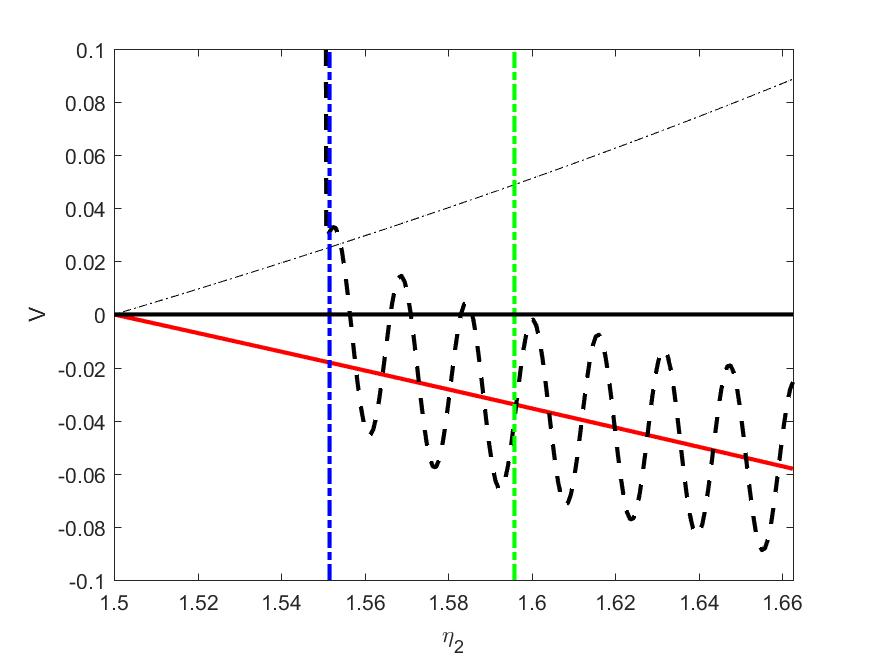
\includegraphics[scale=.25]{twoD/osc_cases.jpg}
\caption{Here we have the parameter ranges for Case I and Case II shown as the right most green vertical line and the bifurcation at the left blue vertical line respectfully.}
\label{fig:twoD_osc_cases}
\end{figure}

\subsection{Case I: $P_0(t)\le -|A|$}
\label{subsec:twoD_highfreqosc_caseI}

We call this the entirely below axis case, with the solution $X_0$ below the axis $V=0$ so that there is no bifurcation. This case helps to simplify the integration in \eqref{eq:twoD_osc_innerintegral} but also helps us to determine when the solution acts differently. Here we use the equilibria of $X$ and $Y$ to define a boundary between Case I and Case II. Under the conditions of this case, the system \eqref{eq:twoD_osc_innerintegral} simplifies to

\begin{equation}\label{eq:twoD_osc_caseIsystem}
\begin{aligned}
{P_0}_t(t) =& -n -\eta_3P_0(t)-(1-\eta_3)Q_0(t),\\
{Q_0}_t(t) =& \eta_1P_0(t)-Q_0(t).
\end{aligned}
\end{equation}

Solving for the equilibria in \eqref{eq:twoD_osc_caseIsystem} results in

\begin{equation*}
Q_0(P_0)=\eta_1P_0,\quad P_0=-\frac{n}{\eta_1(1-\eta_3)+\eta_3}. 
\end{equation*}

Together with these equilibria and with the condition $P_0(t)\le -|A|$, we find the parameter range that distinguishes between Case I and Case II in terms of our inner parameter, which we then rewrite in original coordinates with

\begin{equation}\label{eq:twoD_osc_boundary}
\begin{aligned}
n\ge& (\eta_1(1-\eta_3)+\eta_3)|A|,\\
\eta_2\ge&\eta_1\eta_3+ \frac{(\eta_1(1-\eta_3)+\eta_3)|A|}{\Omega}.
\end{aligned}
\end{equation}

For values of $\eta_2$ below the values given in \eqref{eq:twoD_osc_boundary}, we see the oscillations crossing above the axis $V=0$ and hence use a separate case to deal with this behavior.

\subsection{Case II: $|P_0(t)|<|A|$}
\label{subsec:twoD_highfreqosc_caseII}

We call this the crossing case; here the solution oscillates about the axis $V=0$ while the center of the oscillations approach the axis. With this behavior, we expect a bifurcation to occur in this region and thus we find the equilibria for \eqref{eq:twoD_osc_innerintegral} that determines the location. While this problem is two-dimensional in nature, the integral in \eqref{eq:twoD_osc_innerintegral} is nearly identical to the integral \eqref{eq:oneD_osc_integral} in \autoref{sec:oneD_highfreqosc}. So we may use the ideas of that section here to get an approximate solution. Thus, under the assumptions of this case, we fix a value of $P_0$ and integrate \eqref{eq:twoD_osc_innerintegral} over the regions defined by

\begin{equation*}
R_1=\arccos(P_0/A),\quad R_2=2\pi-\arccos(P_0/A).
\end{equation*}

As in \autoref{sec:oneD_highfreqosc}, the solution to \eqref{eq:twoD_osc_innerintegral} is negative for $P_0(t)$ the region $R\in[0,R_1]$ and alternates sign for the regions $R\in (R_1,R_2]$ and $R\in (R_2,2\pi]$. We follow the same procedure of integrating over each region to get the exact form for \eqref{eq:twoD_osc_innerintegral} with

\begin{equation}\label{eq:twoD_osc_caseIIexact}
\begin{aligned}
{P_0}_t=&-n- \eta_3 P_0(t)-(1-\eta_3)Q_0,\\
{Q_0}_t=&-\frac{2\eta_1}{\pi}\left(\arcsin(P_0/A)P_0+\sqrt{A^2-P_0^2}\right)-Q_0.
\end{aligned}
\end{equation}

Although this is the explicit inner equation from \eqref{eq:twoD_osc_caseIIexact}, this is analytically too complex to find an explicit form for a bifurcation and thus we use a second order Taylor approximation to give an approximate system

\begin{equation}\label{eq:twoD_osc_taylor}
\begin{aligned}
{P_0}_t=&-n -\eta_3 P_0-(1-\eta_3)Q_0,\\
{Q_0}_t=&-\frac{2\eta_1|A|}{\pi}-Q_0-\frac{\eta_1}{\pi|A|}P_0^2.
\end{aligned}
\end{equation}

We solve for the equilibria of \eqref{eq:twoD_osc_taylor} in order to locate the bifurcation. For simplicity, we define $a=\frac{\eta_1}{\pi|A|}$, and $ c=\frac{2\eta_1|A|}{\pi}$, then the equilibria satisfy

\begin{equation}\label{eq:twoD_osc_equilibria}
\begin{aligned}
Q_0(P_0)=&-aP_0^2-c,\\
0=-n+(1-\eta_3)c&-\eta_3 P_0+aP_0^2.
\end{aligned}
\end{equation}

Here the equation for $P_0$ in \eqref{eq:twoD_osc_equilibria} is a quadratic that would have two solutions, with the situation of following the lower branch given by negative solution with

\begin{equation}\label{eq:twoD_osc_innersolution}
P_0=\frac{\eta_3}{2a(1-\eta_3)}- \frac{1}{2a(1-\eta_3)}\sqrt{\eta_3^2+4a(1-\eta_3)(n-c(1-\eta_3))}.
\end{equation}

The equilibrium for $P_0$ in \eqref{eq:twoD_osc_innersolution} are real only for positive discriminant. Then the inner bifurcation, $n_{\text{osc}}$, is given for vanishing discriminant 

\begin{equation}\label{eq:twoD_osc_innerbif}
n_{osc} = \frac{\eta_1(1-\eta_3)|A|}{\pi}\left[2-\left(\frac{\pi\eta_3}{2\eta_1(1-\eta_3)}\right)^2\right].
\end{equation}

Here the equilibria in \eqref{eq:twoD_osc_equilibria} are given in terms of the inner variables. We write the solution for $V$, $T$ and bifurcation, ${\eta_2}_{\text{osc}}$, in the original coordinates

\begin{equation}\label{eq:twoD_osc_innersolnoriginal}
\begin{aligned}
V(t)\sim& \Omega^{-1}\left(P_0-A\cos(\Omega t)\right),\\
T(t)\sim& \eta_1-\Omega^{-1}\left(\frac{\eta_1}{\pi|A|}P_0^2+\frac{2\eta_1|A|}{\pi}+B\cos(\Omega t)\right),
\end{aligned}
\end{equation}

\begin{equation}\label{eq:twoD_osc_bifurcation}
{\eta_2}_{osc} = \eta_1\eta_3+\frac{\eta_1(1-\eta_3)|A|}{\pi\Omega}\left[2-\left(\frac{\pi\eta_3}{2\eta_1(1-\eta_3)}\right)^2\right].
\end{equation}

With \eqref{eq:twoD_osc_bifurcation} we have found the bifurcation induced by the addition of oscillatory forcing in the Stommel model. As we learned from the one-dimensional model in \autoref{sec:oneD_highfreqosc}, the effect of oscillatory forcing is bifurcations where ${\eta_2}_{\text{osc}}>{\eta_2}_{\text{ns}}$. Our result in \eqref{eq:twoD_osc_bifurcation} under the caveat that we restrict the parameters with 

\begin{equation*}
\eta_3 <\frac{2\sqrt{2}\eta_1}{\pi+2\sqrt{2}\eta_1},
\end{equation*}

which is the condition to guarantee the second term in \eqref{eq:twoD_osc_bifurcation} is positive. This restriction is reasonable as generally the parameters have the behaviors of $\eta_3<1$ and $\eta_3\ll \eta_1$ where the thermal variation is much larger in real ocean dynamics than the ratio of relaxation times.

In figure~\ref{fig:twoD_osc_Vnumerics} the numerical solution to \eqref{eq:twoD_canonical} for $V$ and a zoom of the solution around the numerical bifurcation is shown. The static bifurcation diagram is underlayed as well for comparison. We contrast the result in \eqref{eq:twoD_osc_bifurcation} to these numerics and find the bifurcation prediction from our analysis agrees. Notice that there is a bifurcation for $\eta_2>{eta_2}_{\text{ns}}$ with the oscillations present. This causes a region of the static lower branch in $V$ to never be followed.
In figure~\ref{fig:twoD_osc_Tnumerics} the numerical solution to \eqref{eq:twoD_canonical} for $T$ and a zoom in around the bifurcation is shown. Once more, the static bifurcation diagram is underlayed and we have two interesting features to note. Due to the bifurcation in $V$ for $\eta_2>{\eta_2}_{\text{ns}}$, the maximum value of $T$ is never reached in (b).

\begin{figure}[H]
\centering
\begin{subfigure}{.5\textwidth}
  \centering
  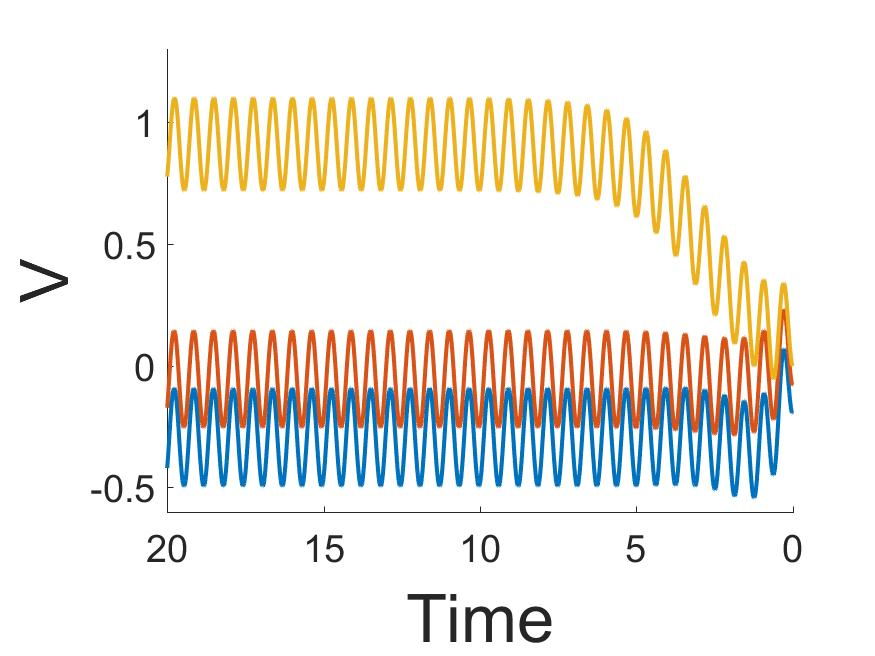
\includegraphics[width=\linewidth]{twoD/osc_Vtimeseries.jpg}
  \caption{}
\end{subfigure}%
\begin{subfigure}{.5\textwidth}
  \centering
  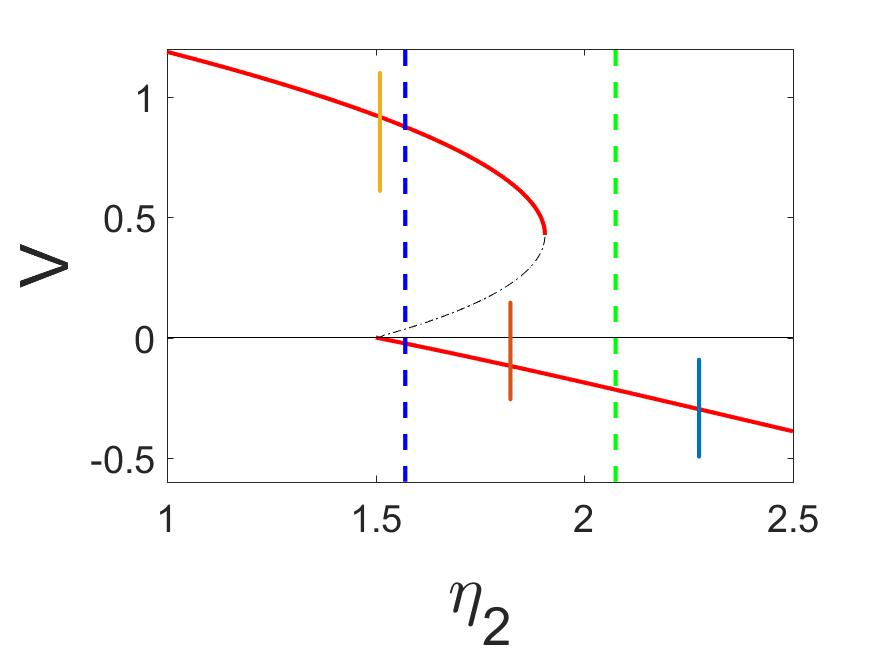
\includegraphics[width=\linewidth]{twoD/osc_bif_diagram.jpg}
  \caption{}
\end{subfigure}
\begin{subfigure}{.5\textwidth}
  \centering
  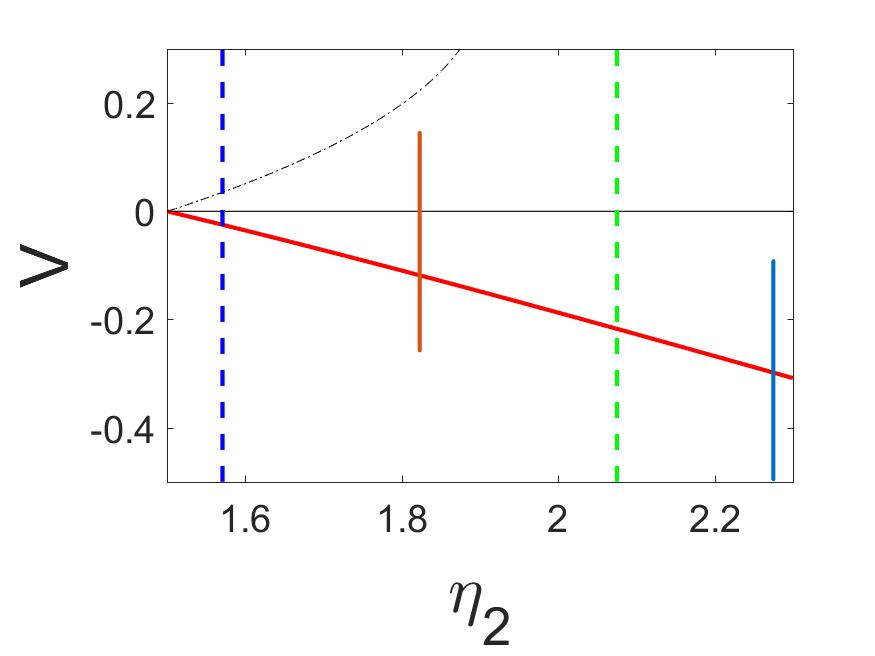
\includegraphics[width=\linewidth]{twoD/osc_bif_diagram_zoom.jpg}
  \caption{}
\end{subfigure}
\caption{In (a) the numerical time series solutions to \eqref{eq:twoD_canonical} is given with parameters in each qualitatively different case of $\eta_2=\{2.3,1.8,1.51\}$ with $\eta_1=4$, $\eta_3=.375$, $A=10$ and $\Omega = 10$. In (b) these same solutions are shown on the bifurcation diagram. In (c) a zoom in closer to the non-smooth bifurcation region where the blue vertical line is the prediction \eqref{eq:twoD_osc_bifurcation} against the black dotted vertical line which is the numerical bifurcation.}
\label{fig:twoD_osc_Vnumerics}
\end{figure}

\begin{figure}[H]
\centering
\begin{subfigure}{.5\textwidth}
  \centering
  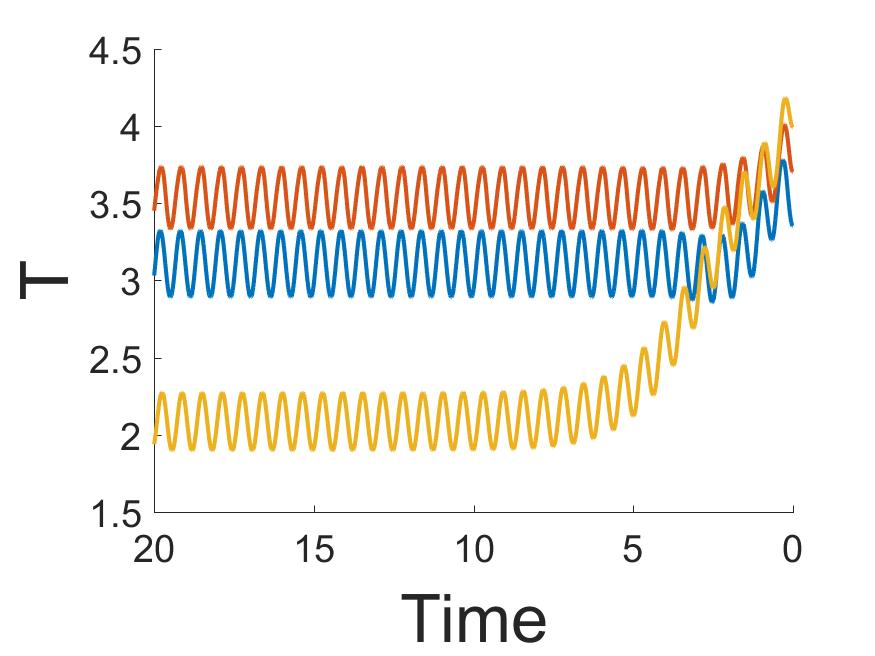
\includegraphics[width=\linewidth]{twoD/osc_Ttimeseries.jpg}
  \caption{}
\end{subfigure}%
\begin{subfigure}{.5\textwidth}
  \centering
  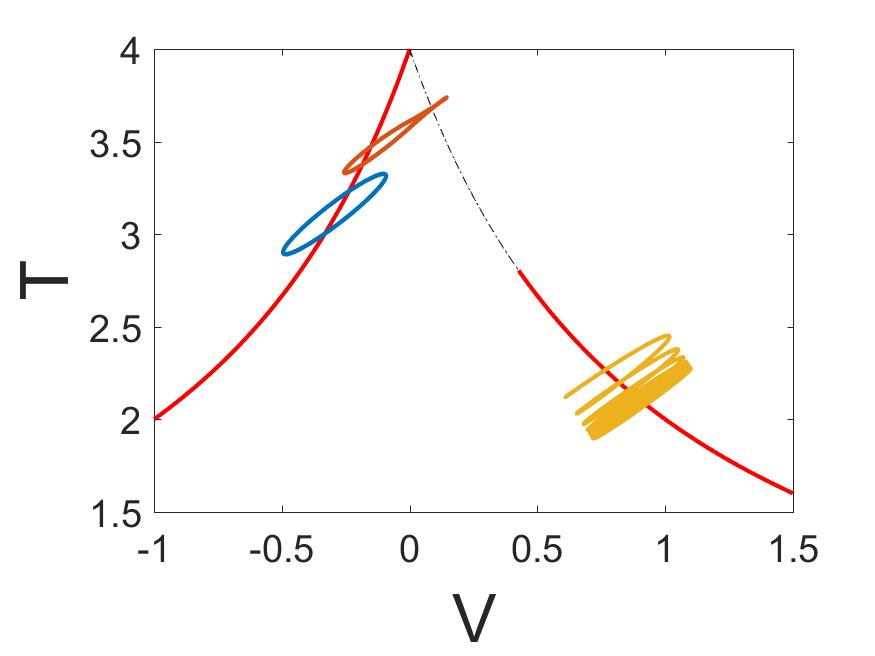
\includegraphics[width=\linewidth]{twoD/osc_bif_Tplot.jpg}
  \caption{}
\end{subfigure}
\begin{subfigure}{.5\textwidth}
  \centering
  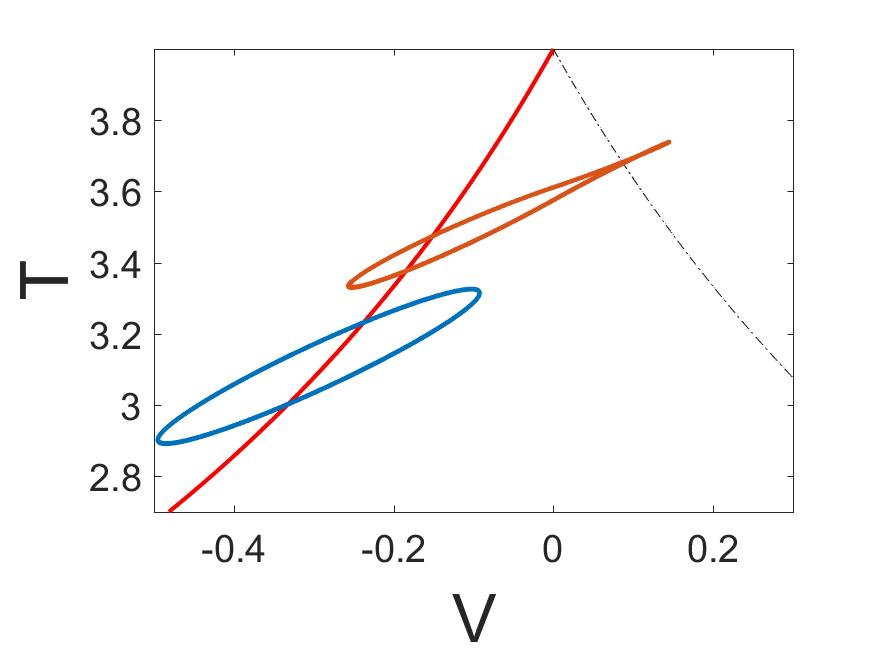
\includegraphics[width=\linewidth]{twoD/osc_bif_Tplot_zoom.jpg}
  \caption{}
\end{subfigure}
\caption{In (a) we have the numerical time series solutions for a qualitatively different cases $\eta_2=\{2.3,1.8,1.51\}$. In (b) we plot these solutions over the standard equilibrium plot for $V$ vs. $T$. In (c) a zoom of the bifurcation area.}
\label{fig:twoD_osc_Tnumerics}
\end{figure}

To evaluate the performance of this prediction, we compare \eqref{eq:twoD_osc_bifurcation} to the numerical bifurcation over a range of $\Omega^{-1}$. In figure~\ref{fig:twoD_osc_epscomp} we allow for this range to be $\Omega^{-1}\in (0,.5)$. For small values, the two agree very well and as we expect, they begin to diverge once the values of $\Omega^{-1}$ become too large from the assumption that $\Omega\gg 1$ and the asymptotics cannot capture the behavior for low frequency oscillations. But under our assumptions, the prediction is performing quite well and resembles the performance of \autoref{sec:oneD_highfreqosc}.

\begin{figure}[H]
\centering
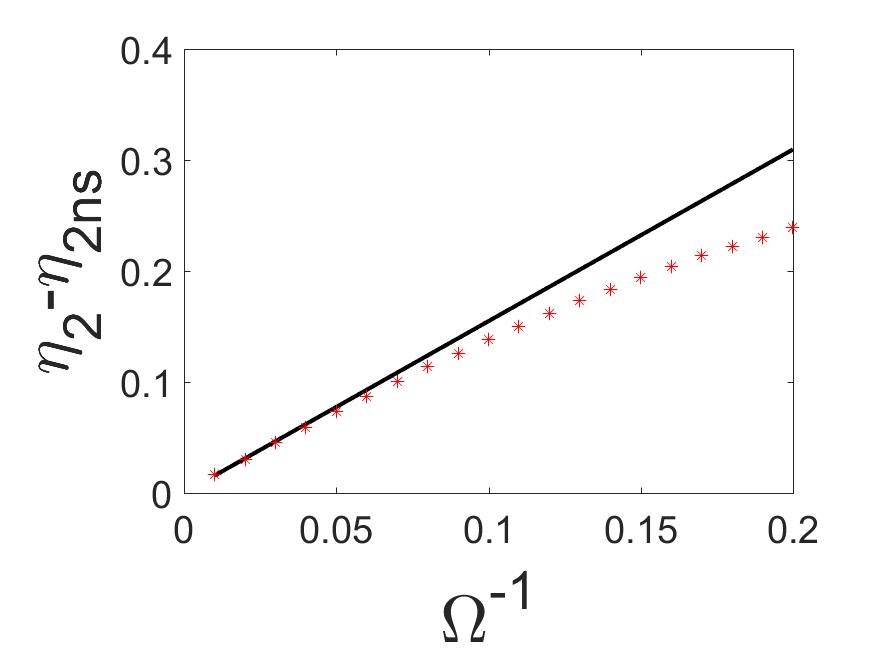
\includegraphics[scale=.25]{twoD/osc_Omegacomp.jpg}
\caption{The numerical tipping vs the estimate with $\eta_1=4$ and $\eta_3=\frac{3}{8}$. The bifurcation is when $V>.5$.}
\label{fig:twoD_osc_epscomp}
\end{figure}

\subsection{Stability}

Since we have a non-autonomous system when $A\not=0$, we approach the stability with a linearized analysis about the equilibria much like in \autoref{sec:oneD_highfreqosc}. To do this, recall from \eqref{eq:twoD_osc_innerintegral} that we found the system

\begin{equation}\label{eq:twoD_osc_stabilityequation}
\begin{aligned}
{P_0}_t =& -n -\eta_3 P_0-(1-\eta_3)Q_0,\\
{Q_0}_t =& -\frac{\eta_1}{2\pi}\int_0^{2\pi}|P_0-A\cos(R)|\, dR - Q_0.
\end{aligned}
\end{equation}

We must consider the stability of solutions over the relative sizes of $P_0(t)$ with Case I: $P_0(t)\le -|A|$ and Case II: $|P_0(t)|\le |A|$.

\subsubsection{Case I: $v_0(t)\le -|A|$}

For this case the entirely below-axis case where the solution spends most of its time away from the axis $V=0$. We expected attraction around the lower branch and thus we expect stability here. Under these conditions, the inner equation \eqref{eq:twoD_osc_stabilityequation} simplifies to the equations

\begin{equation}\label{eq:twoD_osc_stability_caseI_fullinner}
\begin{aligned}
{P_0}_t =& -m -\eta_3 P_0-(1-\eta_3)Q_0,\\
{Q_0}_t =& \eta_1 P_0 - Q_0.
\end{aligned}
\end{equation}

The equilibria of \eqref{eq:twoD_osc_stability_caseI_fullinner} is found with $Q_0(P_0)=\eta_1 P_0$, and thus we find the following one-dimensional equation and equilibrium

\begin{equation}\label{eq:twoD_osc_stability_caseI_red}
{P_0}_t = -n -(\eta_3 +(1-\eta_3))Q_0=f(P_0),\quad Z^0 = -\frac{n}{\eta_3+\eta_1(1-\eta_3)}.
\end{equation}

Now we consider a simple linear perturbation about this equilibrium with $P_0(t)= Z^0+U(t)$ where $\lVert U(t) \rVert \ll 1$. Our standard Taylor expansion about the equilibrium $Z^0$ results in

\begin{equation}\label{eq:twoD_osc_stability_caseI_perteq}
\begin{aligned}
f(P_0)=&f(Z^0)+f_{P_0}(Z^0)(P_0-Z^0)+O((P_0-Z^0)^2),\\
U_t =& -(\eta_3+\eta_1(1-\eta_3))U
\end{aligned}
\end{equation}

From \eqref{eq:twoD_osc_stability_caseI_perteq} we now conclude the equilibrium $Z^0$ is hyperbolic and asymptotically stable due to the exponential decay in perturbations. Thus we find that no bifurcation occurs for this case which agrees with our findings for this case in the analysis for $\eta_2$ in \eqref{eq:twoD_osc_boundary}

\begin{equation*}
\eta_2 \ge \eta_1\eta_3 +\frac{(\eta_3+\eta_1(1-\eta_3))|A|}{\Omega}.
\end{equation*}


\subsubsection{Case II: $|P_0(t)|<|A|$}

We called this case the crossing case and here the solution experiences the non-smooth behavior when it crosses $V=0$. We expect the stability to fail under these conditions and we discovered in the analysis that the crossing $V=0$ gives \eqref{eq:twoD_osc_stabilityequation} in the form

\begin{equation}\label{eq:twoD_osc_stability_caseII_full}
\begin{aligned}
{P_0}_t =& -n-\eta_3 P_0-(1-\eta_3)Q_0,\\
{Q_0}_t =& -\frac{2\eta_1|A|}{\pi}-\frac{\eta_1}{\pi |A|}P_0^2-Q_0.
\end{aligned}
\end{equation}

As we search for the equilibria of \eqref{eq:twoD_osc_stability_caseII_full}, we find the equilibrium for $Q_0$ in terms of $P_0$  

\begin{equation*}
Q_0(P_0)=-\frac{2\eta_1|A|}{\pi}-\frac{\eta_1}{\pi |A|}P_0^2
\end{equation*}

which then gives the following inner equation with the chosen equilibrium for $P_0<0$

\begin{equation}\label{eq:twoD_osc_stability_caseII_inner}
\begin{aligned}
{P_0}_t=&-n+\frac{2\eta_1(|A|}{\pi}-\eta_3 P_0+\frac{\eta_1}{\pi |A|}P_0^2=f(P_0),\\
Z^0=&\frac{\pi |A|}{2\eta_1(1-\eta_3)}\left(\eta_3-\sqrt{\frac{4\eta_1(1-\eta_3)}{\pi|A|}(n-n_{\text{osc}})}\right).
\end{aligned}
\end{equation}

For simplicity we write $Z^0$ in terms of the inner bifurcation $n_{text{osc}}$ we found in the analysis with \eqref{eq:twoD_osc_innerbif}. We now consider a simple linear perturbation about this equilibrium in \eqref{eq:twoD_osc_stability_caseII_inner} with $P_0(t)=Z^0+U(t)$ where $\lVert U(t)\rVert\ll 1$. The standard Taylor expansion about the equilibrium is thus

\begin{equation}\label{eqLtwoD_osc_stability_caseII_perturb}
\begin{aligned}
f(P_0)=&f(Z^0)+f_{P_0}(Z^0)(P_0-Z^0)+O((P_0-Z^0)^2),\\
U_t=&- 2\sqrt{\frac{\eta_1(1-\eta_3)}{\pi|A|}(n-n_{\text{osc}})}U.
\end{aligned}
\end{equation}

Thus with \eqref{eqLtwoD_osc_stability_caseII_perturb} we learn that the perturbations $U(t)$ decay exponentially as long as the square-root is non-zero and we restrict our attention to real solutions so that our perturbations are real. Thus we have that $Z^0$ is a hyperbolic and asymptotically stable equilibrium for $P_0$ and thus we find stability in $Q_0$ as well. This gives stability for this region but we lose this stability once the square-root becomes zero, here when

\begin{equation*}
n_{osc} = \frac{\eta_1(1-\eta_3)|A|}{\pi}\left[2-\left(\frac{\pi\eta_3}{2\eta_1(1-\eta_3)}\right)^2\right].
\end{equation*}

This says the equilibrium $Z^0$ at this point is non-hyperbolic which is indicative of a bifurcation. This is in agreement with our analysis and thus we can say that the value found in \eqref{eq:twoD_osc_bifurcation} is the bifurcation under the oscillatory forcing.


\section{Slow Variation with Oscillatory Forcing}
\label{sec:twoD_slowosc}

With the one-dimensional model solved and both the slowly varying and high oscillatory two-dimensional components analyzed, we have all of the tools needed to analyze the full system \eqref{eq:twoD_canonical} with both $\epsilon \ll 1$ and $A,B\sim O(1)$ simultaneously. This is the most general setting we discuss in this thesis where we account for both a slowly varying $\eta_2$ that leads to abrupt changes seen in \cite{alley2003abrupt,marotzke2000abrupt,rahmstorf2000thermohaline} as well as oscillatory forcing in both equations in \eqref{eq:twoD_canonical} seen in \cite{roberts2017relaxation,huybers2005obliquity}. We search for the interaction of these mechanisms in the physical Stommel model. Under the framework of slowly varying parameters we expect to find tipping instead of a bifurcation and hence our method for finding the tipping point follows a mixture of both \autoref{sec:twoD_slow} and \autoref{sec:twoD_highfreqosc}. This procedure dictates that we search for inner behavior about the non-smooth bifurcation and to do so we need to solve the inner equation and estimate when this solution abruptly transitions towards the upper branch. Ultimately, we provide a solution that captures the abrupt change from the lower stable branch to the upper branch in the full Stommel model.

To begin, we take our standard approach of following the lower branch towards the non-smooth behavior with $V<0$ in \eqref{eq:twoD_canonical} which gives the following system  

\begin{equation}\label{eq:twoD_slowosc_outereqs}
 \begin{aligned}
   \dot{V} & =  \eta_1-\eta_2-T+\eta_3(T-V)+V^2+A\sin(\Omega t), \\
   \dot{T} & =  \eta_1-T(1-V)+B\sin(\Omega t),  \\
  \dot{\eta_2}  & =  -\epsilon.
  \end{aligned}
\end{equation}

As in \autoref{sec:oneD_slowosc}, we write the frequency in terms of the slow variation, $\Omega = \epsilon^{-\lambda}$ with exponent $\lambda>0$. This assumption allows us to find the irelative influence of the slowly varying parameter and fast oscillations on the tipping. We notice in \eqref{eq:twoD_slowosc_outereqs} that there is variation on a slow scale in $\eta_2(t)$ and on a fast scale in $\sin(\Omega t)$, so this suggests a multiple scales approach with 'slow' time $\tau = \epsilon t$ and 'fast' time $R=\epsilon^{-\lambda}t$. Using this approach in \eqref{eq:twoD_slowosc_outereqs} yields

\begin{equation}\label{eq:twoD_slowosc_multiouter}
 \begin{aligned}
V_R+\epsilon^{\lambda+1}V_\tau & = \epsilon^{\lambda} \left(\eta_1-\eta_2-		T+\eta_3(T-V)+V^2+A\sin(R)\right), \\
T_R+\epsilon^{\lambda+1}T_\tau & = \epsilon^{\lambda}\left( \eta_1-T(1-		  V)+B\sin(R)\right),  \\
	{\eta_2}_\tau  & =  -1.
\end{aligned}
\end{equation}
  
To approach the solution to the outer equations in \eqref{eq:twoD_slowosc_multiouter}, we use an asymptotic expansion using both $\epsilon^\lambda$ and integer powers as we have not specified the range of $\lambda$ and both could be significant. Thus our expansion is

\begin{equation}\label{eq:twoD_slowosc_outerexpansion}
	\begin{aligned}
		V(\tau,R)\sim& V_0(\tau,R)+\epsilon^\lambda 	V_1(\tau,R)+O(\epsilon^{2\lambda},\epsilon^{\lambda+1}),\\
        T(\tau,R)\sim& T_0(\tau,R)+\epsilon^\lambda T_1(\tau,R)+O(\epsilon^{2\lambda},\epsilon^{\lambda+1}).
	\end{aligned}
\end{equation}

Here we substitute \eqref{eq:twoD_slowosc_outerexpansion} into \eqref{eq:twoD_slowosc_multiouter} to give

\begin{equation*}
\begin{aligned}
{V_0}_R+\epsilon^{\lambda+1}{V_0}_\tau+\epsilon^\lambda {V_1}_R+\ldots=&\begin{aligned}[t]&
\epsilon^\lambda \left(\eta_1-\eta_2-T+\eta_3(T_0-V_0)+V_0^2+A\sin(R)\right)\\
&+\epsilon^{2\lambda}\left(-\eta_3 V_1-(1-\eta_3)T_1+2V_0V_1\right)+\ldots
\end{aligned}\\
{T_0}_R+\epsilon^{\lambda+1}{T_0}_\tau+\epsilon^\lambda {T_1}_R+\ldots=&\begin{aligned}[t]&
\epsilon^\lambda\left( \eta_1-T_0(1-V_0)+B\sin(R)\right)\\
&+\epsilon^{2\lambda}\left(-T_1+T_0V_1+T_1V_0\right)+\ldots
\end{aligned}
\end{aligned}
\end{equation*}

Separating the equation at each order of $\epsilon$ then gives the following sets of equations

\begin{align}
\label{eq:twoD_slowosc_outerO1}
O(1):\quad & \begin{cases}
	{V_0}_R =&  0, \\
	{T_0}_R =&  0,\\
\end{cases}\\
\label{eq:twoD_slowosc_outerO2}
O(\epsilon^\lambda):\quad & \begin{cases}
	{V_1}_R = & \eta_1-\eta_2(\tau) +\eta_3(T_0-V_0)-T_0+V_0^2+A\sin(R),\\
	{T_1}_R =&  \eta_1-T_0(1-V_0)+B\sin(R),
\end{cases}\\
\label{eq:twoD_slowosc_outerO3}
O(\epsilon^{2\lambda}):\quad & \begin{cases}
	{V_2}_R+\epsilon^{1-\lambda}{V_0}_\tau = & \eta_3(T_1-V_1)-T_1+2V_0V_1,\\
	{T_2}_R +\epsilon^{1-\lambda}{T_0}_\tau =&  -T_1(1-V_0)+T_0V_1,
\end{cases}
\end{align}

Here we consider a $\lambda$ where the next order in \eqref{eq:twoD_slowosc_outerexpansion} is $O(\epsilon^{2\lambda})$. Similar results follow from a choice in $\lambda$ where $O(\epsilon^{\lambda+1})<O(\epsilon^{2\lambda})$. From \eqref{eq:twoD_slowosc_outerO1} the leading order terms in our expansion are only dependent on 'slow' time, $V_0=V_0(\tau)$ and $T_0=T_0(\tau)$. The solutions of \eqref{eq:twoD_slowosc_outerO2} and \eqref{eq:twoD_slowosc_outerO3} are found in \autoref{app:twoD}, giving the outer solution 

\begin{equation}\label{eq:twoD_slowosc_outersoln}
\begin{aligned}
V\sim& V_0 + \frac{\epsilon({V_0}_\tau(1-V_0)+(1-\eta_3){T_0}_\tau)}{(1-\eta_3)T_0+(2V_0-\eta_3)(1-V_0)}-\epsilon^\lambda A \cos(\Omega t),\\
T\sim& T_0 + \frac{\epsilon {T_0}_\tau}{1-V_0}-\frac{\epsilon T_0({V_0}_\tau(1-V_0)+(1-\eta_3){T_0}_\tau)}{(1-\eta_3)T_0(1-V_0)+(2V_0-\eta_3)(1-V_0)^2}-\epsilon^\lambda B \cos(\Omega t),
\end{aligned}
\end{equation}

where $V_0$ and $T_0$ are the same leading order solutions from the slowly varying Stommel model in \autoref{sec:twoD_slow}. Unfortunately the common theme of the Stommel model is that these outer solutions are complex but it is clear the outer expansion breaks down for $V_0\ll 1$. Thus we derive a scaling for the inner equations analogous to that of \autoref{sec:oneD_slowosc}.

For simplicity, we assume that the scaling for both $V$ and $T$ are the same, but this isn't necessary to arrive at the same conclusion. Hence we rescale about the bifurcation point $(V,T,\eta_2)=(0,\eta_1,\eta_1\eta_3)$ with

\begin{equation}\label{eq:twoD_slowosc_general_scaling}
V=\epsilon^\alpha X, \quad T=\eta_1+\epsilon^\alpha Y ,\quad \eta_2(t)=\eta_1\eta_3+\epsilon^\beta n(t),
\end{equation}

where both $\alpha>0$ and $\beta>0$ allow for this to be a local scaling. Applying the scalings in \eqref{eq:twoD_slowosc_general_scaling} to the full Stommel model \eqref{eq:twoD_canonical} gives

\begin{equation}\label{eq:twoD_slowosc_innerscaled}
\begin{aligned}
\epsilon^\alpha \dot{X}=& -\epsilon^\beta n(t)-\epsilon^\alpha (X+(1-\eta_3)Y) - \epsilon^{2\alpha}X|X| +A\sin(\epsilon^{-\lambda}t),\\
\epsilon^\alpha \dot{Y}=&-\epsilon^\alpha(\eta_1|X|+Y)+\epsilon^{2\alpha}|X|Y +B\sin(\epsilon^{-\lambda} t)\\
\dot{n}=&-\epsilon^{1-\beta}.
\end{aligned}
\end{equation}

From \eqref{eq:twoD_slowosc_innerscaled} it is apparent that there is still 'fast' behavior within the oscillations. Also note that due to the scaling in \eqref{eq:twoD_slowosc_general_scaling}, the local variables 'slow' behavior has been moved into the regular time $t$. To flesh out the particular choice in $\alpha$, we then take a multiple scales approach to capture the oscillations with $t$ and $R=\epsilon^{-\lambda}t$.  This choice comes with the ambiguity in $\beta$ and is discussed further below. Applying the multiple scales in \eqref{eq:twoD_slowosc_innerscaled} results in

\begin{equation}\label{eq:twoD_slowosc_innergeneral}
\begin{aligned}
\epsilon^{\alpha-\lambda} X_R+\epsilon^{\alpha}X_t=& -\epsilon^{\beta}n(t)-\epsilon^{\alpha}(X+(1-\eta_3)Y)-\epsilon^{2\alpha}X|X|+A\sin(R),\\
\epsilon^{\alpha-\lambda}Y_R + \epsilon^{\alpha}Y_t =&- \epsilon^\alpha(\eta_1|X|+Y)-\epsilon^{2\alpha}|X|Y +B\sin(R)\\
n_t=&-\epsilon^{1-\beta}.
\end{aligned}
\end{equation}

Here we balance the leading order terms in each equation of \eqref{eq:twoD_slowosc_innergeneral}, $\epsilon^{\alpha-\lambda}X_R$ and $A\sin(R)$ as well as $\epsilon^{\alpha-\lambda}Y_R$ with $B\sin(R)$, which gives us that $\alpha=\lambda$ and confirms that the scales $V$ and $T$ are the same. The scaling for $\eta_2$ has yet to be determined and could have multiple possibilities depending on $\lambda$, but due to this choice in $\alpha$ we expect the oscillatory term to persist in the inner asymptotic expansion of \eqref{eq:twoD_canonical} regardless of choice in $\lambda$.

We use a multiple scales approach with $t$ and $R=\epsilon^{-\lambda}t$ on the full Stommel model \eqref{eq:twoD_canonical} along with the general scaling \eqref{eq:twoD_slowosc_general_scaling} on $\eta_2$ which gives

\begin{equation}\label{eq:twoD_slowosc_general_outermulti}
\begin{aligned}
V_R+\epsilon^{\lambda}V_t =& -\epsilon^{\lambda+\beta}n(t)-\epsilon^{\lambda}(\eta_1-\eta_1\eta_3+\eta_3(T-V)-T-V|V|+A\sin(R)),\\
T_R+\epsilon^{\lambda}T_t =& \epsilon^\lambda(\eta_1-T(1+|V|)+B\sin(R)),\\
n_t =&-\epsilon^{1-\beta}.
\end{aligned}
\end{equation}

In \autoref{sec:oneD_slowosc} the results depended on the relative size of the slow variation with respect to the oscillations. The distinction in that case was when $\lambda\le1$ where a mixture between the slow variation and oscillations influence the tipping or $\lambda>1$ where the slow variation dominates the tipping. We find a similar distinction here and hence consider a separate asymptotic expansion for the following Case I: $\lambda\le 1$ and Case II: $\lambda >1$ to find an accurate classification of behavior for the full Stommel model.

\subsection{Case I: $\lambda \le 1$}

We call this the mixed effects case where there is significant influence from both slow variation and fast oscillations due to the size of $\lambda$. Here we cannot determine what the next term in the expansion should be and thus we choose a general expansion with

\begin{equation}\label{eq:twoD_slowosc_caseI_expansion}
\begin{aligned}
V(t,R)\sim& \epsilon^{\lambda} X_0(t,R)+\epsilon^q X_1(t,R)+\ldots\\
T(t,R)\sim& \eta_1+\epsilon^{\lambda} Y_0(t,R)+\epsilon^q Y_1(t,R)+\ldots
\end{aligned}
\end{equation}

with $q>\lambda$ to be consist with our analysis thus far. Substituting \eqref{eq:twoD_slowosc_caseI_expansion} into \eqref{eq:twoD_slowosc_general_outermulti} then gives the governing dynamics for this case

\begin{equation*}
\begin{aligned}
 {X_0}_R+\epsilon^{\lambda}{X_0}_t+\epsilon^{q-\lambda} {X_1}_R\ldots={} & -\epsilon^{\beta}n(t)-\epsilon^{\lambda} (\eta_3X_0+(1-\eta_3)Y_0) \\
&-\epsilon^{2\lambda}(X_0+\epsilon^{q-\lambda} X_1+\ldots)|X_0+\epsilon^{q-\lambda} X_1+\ldots|\\
& - \epsilon^{q}(\eta_3X_1+(1-\eta_3)Y_1) + A\sin(R) +\ldots
\end{aligned}
\end{equation*}

\begin{equation*}
\begin{aligned}
{Y_0}_R+\epsilon^{\lambda}{Y_0}_t+\epsilon^{q-\lambda} {Y_1}_R+\ldots= &-\epsilon^\lambda(\eta_1| X_0 +\epsilon^{q-\lambda} X_1+\ldots|+ Y_0+\epsilon^{q-\lambda} Y_1+\ldots)\\
&+\epsilon^{2\lambda}|X_0 +\epsilon^{q-\lambda} X_1+\ldots|(Y_0+\epsilon^{q-\lambda} Y_1+\ldots)\\
&+ B\sin (R)+\ldots
\end{aligned}
\end{equation*}

We separate by the distinct orders of $\epsilon$ to find the following equations at each order

\begin{align} \label{eq:twoD_slowosc_caseI_O1}
O(1):\, &\begin{cases}
	{X_0}_R =&  A\sin(R), \\
	{Y_0}_R =&  B\sin(R),\\
\end{cases}\\ \label{eq:twoD_slowosc_caseI_O2}
O(\epsilon^\lambda): \, & \begin{cases}
	\epsilon^{q-2\lambda}{X_1}_R+{X_0}_t =&  -\epsilon^{\beta-\lambda} n(t) -\eta_3 X_0-(1-\eta_3)X_0, \\
	\epsilon^{q-2\lambda}{Y_1}_R+{Y_0}_t =&  -\eta_1|X_0|-Y_0.\\
\end{cases}
\end{align}

We learn from \eqref{eq:twoD_slowosc_caseI_O2} that $q= 2\lambda$ balances the terms, which implies that $\lambda> \frac{1}{2}$ for an expansion to be found. If $\lambda\le \frac{1}{2}$ then we would need to include the quadratic terms in $O(\epsilon^\lambda)$ and our equations would just be the same as the full Stommel model \eqref{eq:twoD_canonical}. This indicated that our local approximation would no longer hold and that the high frequency assumption is failing. Without this, the physical behavior of the problem is qualitatively different and this we explore in the conclusion in \autoref{chap:conclusion}. On this range of $\lambda$, there are two choices for the scaling of $\eta_2$ with $\beta=1$ or $\beta=\lambda$. The advantage to choosing $\beta=\lambda$ is that the equation \eqref{eq:twoD_slowosc_caseI_O2} is simple, but the slow variation equation has the form $n_t = -\epsilon^{1-\lambda}$ and implies a slower time scale. On the other hand, $\beta=1$ keeps a small coefficient on $n$ in \eqref{eq:twoD_slowosc_caseI_O2} but gives the slow variation equation as $n_t=-1$, which allows the time scale $t$ to be used. Both of these choices result in the same approximation of the tipping point in original coordinates, so here we choose $\beta=1$ for convenience. From \eqref{eq:twoD_slowosc_caseI_O1} we find the appropriate form of the leading order terms, $X_0=P_0(t)-A\cos(R)$ and $Y_0=Q_0(t)-B\cos(R)$. Using these forms for the leading order term and applying the Fredholm alternative \eqref{eq:Fredholm} to \eqref{eq:twoD_slowosc_caseI_O2} we find 

\begin{equation}\label{eq:twoD_slowosc_caseI_fullinner}
\begin{aligned}
{P_0}_t =&  -\epsilon^{1-\lambda} n(t) -\eta_3 P_0-(1-\eta_3)Q_0, \\
{Q_0}_t =&  -\frac{\eta_1}{2\pi}\int_0^{2\pi}|P_0(t)-A\cos(R)|\,dR-Q_0,\\
n_t =& -1.
\end{aligned}
\end{equation}

We learned in \autoref{sec:twoD_highfreqosc} that we must approach the integration with the relative size of $P_0(t)$ to the amplitude of oscillation $A$ in mind as these sizes determine the contributions of the integral in \eqref{eq:twoD_slowosc_caseI_fullinner}. We consider these sizes of $P_0(t)$ as Sub-Case I: $P_0(t)\le -|A|$ and Sub-Case II:$|P_0(t)|<|A|$ similar to \autoref{sec:twoD_highfreqosc}. These cases let $P_0-A\cos(R)$ either stay entirely below $V=0$ or change signs respectively and allow the integration to have two distinct forms.

\subsubsection{Sub-Case I: $P_0(t)\le -|A|$}

We call this the below-axis sub-case where the solution $P_0(t)$ is entirely below the axis $V=0$ and this means the full solution $X_0$ has oscillations far from crossing. Under these conditions we don't expect any tipping behavior as the solution is far from $V=0$, but we may use this size of $P_0(t)$ to find the range of $\eta_2$ that distinguishes these cases. With $P_0(t)\le -|A|$, we find \eqref{eq:twoD_slowosc_caseI_fullinner} simplifies to

\begin{equation}\label{eq:twoD_slowosc_subcaseI_full}
\begin{aligned}
{P_0}_t =&  -\epsilon^{1-\lambda} n(t) -\eta_3 P_0-(1-\eta_3)Q_0, \\
{Q_0}_t =&  \eta_1 P_0-Q_0.
\end{aligned}
\end{equation}

We have the means available to solve \eqref{eq:twoD_slowosc_subcaseI_full} as it takes the form of an equation we have seen in \autoref{sec:twoD_slow}, but instead we search for when the pseudo-equilibrium fails the assumption of this sub-case. This results in the parameter range between these sub-cases and taking this approach is more convenient than solving the system. Here the form of the pseudo-equilibria is simple to find as $Q_0(P_0) = \eta_1P_0$ and thus 

\begin{equation*}
P_0(t) = -\epsilon^{1-\lambda}\frac{n(t)}{\eta_3+\eta_1(1-\eta_3)}.
\end{equation*}

But we recall that for this sub-case $P_0(t)\le -|A|$, which gives the range for $n$ and we rewrite this in the original coordinates of $\eta_2$ with

\begin{equation}\label{eq:twoD_slowosc_subcaseboundary}
\begin{aligned}
\epsilon n \ge & \epsilon^\lambda (\eta_3+\eta_1(1-\eta_3))|A|,\\
\eta_2 \ge& \eta_1\eta_3 +\frac{(\eta_3+\eta_1(1-\eta_3))|A|}{\Omega}.
\end{aligned}
\end{equation}

With the parameter range \eqref{eq:twoD_slowosc_subcaseboundary}, we now have an effective region for Sub-Case I and have the range for Sub-Case II in terms of the parameter $\eta_2$.

\subsubsection{Sub-Case II: $|P_0(t)|\le |A|$}

We call this the crossing sub-case and under these conditions we see the integral in \eqref{eq:twoD_slowosc_caseI_fullinner} is more complex. As this contribution changes, there is an increasing effect on the system and it is here that we anticipate the tipping to occur. In \autoref{sec:oneD_slowosc}, we found a similar integral to \eqref{eq:twoD_slowosc_caseI_fullinner} that we could evaluate with the assumption that $A\sim O(1)$. We find that the assumptions that allowed for evaluation of the integral in \eqref{eq:oneD_slowosc_caseIintegral} from \autoref{sec:oneD_slowosc} still hold here with a 'fast' time $R$ that is sufficiently large due to the high frequency. We then follow the approach from \autoref{sec:oneD_slowosc} by integrating with $R_1=\arccos(P_0/A)$ and $R_2 = 2\pi-\arccos(P_0/A)$ analogous to $T_1$ and $T_2$ from \autoref{sec:oneD_slowosc} Case I and then taking a quadratic Taylor approximation as in \eqref{eq:oneD_slowosc_subcaseIItaylor} gives

\begin{equation}\label{eq:twoD_slowosc_subcaseII_taylor}
\begin{aligned}
{P_0}_t =& -\epsilon^{1-\lambda}n(t)-\eta_3 P_0(s)-(1-\eta_3)Q_0\\
{Q_0}_t =&-\frac{2\eta_1|A|}{\pi}-\frac{\eta_1}{\pi|A|}P_0^2-Q_0.
\end{aligned}
\end{equation}

Here the form in \eqref{eq:twoD_slowosc_subcaseII_taylor} is known as a quadratic two-dimensional Riccati-type equation. We recall the assumption that the solution to the equation for $T$ to be in terms of $V$ was realistic to the THC, so any behavior that we are interested in lies within the dynamics for $V$, or it's inner counterpart $X$. For this reason, we choose to approximate by reducing \eqref{eq:twoD_slowosc_subcaseII_taylor} to a one-dimensional model by assuming our equation for $Q_0$ is in pseudo-equilibrium with 

\begin{equation}\label{eq:twoD_slowosc_subcaseII_equilreduction}
{Q_0}(P_0) =  -\frac{2\eta_1|A|}{\pi}-\frac{\eta_1}{\pi|A|}P_0^2.
\end{equation}

The resulting reduced system from introducing the equilibrium \eqref{eq:twoD_slowosc_subcaseII_equilreduction} into the leading order inner equation \eqref{eq:twoD_slowosc_subcaseII_taylor} is then

\begin{equation}\label{eq:twoD_slowosc_subcaseII_reducedeq}
\begin{aligned}
{P_0}_t =& -\epsilon^{1-\lambda}n(t)+\frac{2\eta_1(1-\eta_3)|A|}{\pi}-\eta_3P_0+\frac{\eta_1}{\pi|A|}P_0^2,\\
n_t=&-1.
\end{aligned}
\end{equation}

We rewrite the differentiation in \eqref{eq:twoD_slowosc_subcaseII_reducedeq} in terms of parameter $n$ giving 

\begin{equation} \label{eq:twoD_slowosc_subcaseII_reducedn}
\begin{aligned}
{P_0}_n =& \epsilon^{1-\lambda} n -\frac{2\eta_1(1-\eta_3)|A|}{\pi}+\eta_3 P_0-\frac{\eta_1(1-\eta_3)}{\pi|A|}P_0^2.\\
\end{aligned}
\end{equation}

Now \eqref{eq:twoD_slowosc_subcaseII_reducedn} is in a form when the result from Zhu \& Kuske \eqref{eq:intro_Zhueq} applies. Thus we determine that \eqref{eq:twoD_slowosc_subcaseII_reducedn} is an Airy-type equation and that the tipping point follows with \eqref{eq:intro_Zhuresult}. We write the solution in original coordinates and obtain results similar to previous sections with

\begin{equation}\label{eq:twoD_slowosc_subcaseII_tipping}
\begin{aligned}
n_{\text{tip}} =& -\epsilon^{(\lambda-1)/3}\left(\frac{\pi|A|}{\eta_1(1-\eta_3)}\right)^{1/3}(2.33810)+\epsilon^{\lambda-1}\frac{\eta_1(1-\eta_3)|A|}{\pi}\left(2-\left(\frac{\pi\eta_3}{2\eta_1(1-\eta_3)}\right)^2\right),\\
{\eta_2}_{\text{tip}} =& \epsilon^{(\lambda-1)/3}\left(\frac{\pi|A|}{\eta_1(1-\eta_3)}\right)^{1/3}\mu_{\text{smooth}}+{\eta_2}_{\text{osc}}
\end{aligned}
\end{equation}

We conclude that the tipping point in \eqref{eq:twoD_slowosc_subcaseII_tipping} has a similar fom as the tipping point found with \eqref{eq:oneD_slowosc_caseItipping} in \autoref{sec:oneD_slowosc} where we found a weighted average between the smooth tipping and the oscillatory bifurcation for this range of $\lambda$. We also found in \eqref{eq:twoD_slowosc_caseI_O2} that any choice for $\lambda\le\frac{1}{2}$ gave equations that can not be studied using the multiple scales approach in this section. This heuristically makes sense since for $\lambda\le \frac{1}{2}$ we have low frequency oscillations with our polynomial relationship and the contributions to the dynamics from this behavior require a different approach than presented in this paper. For more, see Zhu \& Kuske \cite{zhu2015tipping} for an example of a low-frequency method.

\subsection{Case II: $\lambda>1$}

We call this case the slow dominant case; here we expect integer powers of $\epsilon$ to appear due to the $O(\epsilon^\lambda)$ being quite small for this range of $\lambda$ and thus we choose the expansion 

\begin{equation}\label{eq:twoD_slowosc_caseII_expansion}
\begin{aligned}
V(t,R) \sim& \epsilon X_0(t,R)+\epsilon^\lambda X_1(t,R)+\epsilon^q X_2(t,R)+\ldots\\
T(t,R) \sim& \epsilon Y_0(s,R) + \epsilon^\lambda Y_1(t,R) +\epsilon^q Y_2(t,R)+\ldots
\end{aligned}
\end{equation}

Substituting \eqref{eq:twoD_slowosc_caseII_expansion} into \eqref{eq:twoD_slowosc_general_outermulti} then gives

\begin{equation*}
\begin{aligned}
\epsilon {X_0}_R+\epsilon^{\lambda+1}{X_0}_t+\epsilon^\lambda {X_1}_R+\ldots={} & -\epsilon^{\lambda+\beta}n(t)-\epsilon^{\lambda+1} (\eta_3X_0+(1-\eta_3)Y_0) \\
&-\epsilon^{\lambda+2}(X_0+\epsilon^{q-\lambda} X_1+\ldots)|X_0+\epsilon^{q-\lambda} X_1+\ldots|\\
& - \epsilon^{2\lambda}(\eta_3X_1+(1-\eta_3)Y_1) + \epsilon^\lambda A\sin(R),
\end{aligned}
\end{equation*}

\begin{equation*}
\begin{aligned}
\epsilon {Y_0}_R+\epsilon^{\lambda+1}{Y_0}_t+\epsilon^\lambda {Y_1}_R+\ldots=& -\epsilon^{\lambda+1}(\eta_1|X_0 +\epsilon^{\lambda-1} X_1+\epsilon^{q-1} X_2+\ldots|- Y_0-\epsilon^{\lambda-1} Y_1+\ldots)\\
&+\epsilon^2|X_0 +\epsilon^{\lambda-1} X_1+\epsilon^{q-1} X_2+\ldots|(Y_0 +\epsilon^{\lambda-1} Y_1+\ldots)\\
&+\epsilon^\lambda B \sin (R).
\end{aligned}
\end{equation*}

Here we separate by each distinct order of $\epsilon$ to find the following equations at each order of $\epsilon$

\begin{align} \label{eq:twoD_slowosc_caseII_O1}
O(\epsilon):\, &\begin{cases}
	{X_0}_R =& 0, \\
	{Y_0}_R =& 0,\\
\end{cases}\\ \label{eq:twoD_slowosc_caseII_O2}
O(\epsilon^\lambda): \, & \begin{cases}
	{X_1}_R =& A\sin(R), \\
	{Y_1}_R =& B\sin(R),\\
\end{cases}\\
\label{eq:twoD_slowosc_caseII_O3}
O(\epsilon^{\lambda+1}):\, &\begin{cases}
	\epsilon^{q-\lambda-1}{X_2}_R+{X_0}_t =& -\epsilon^{\beta-1}n(t)-\eta_3X_0-(1-\eta_3)Y_0, \\
	\epsilon^{q-\lambda-1}{Y_2}_R+{Y_0}_t =& -\eta_1|\epsilon^{\lambda}|X_0+\epsilon^{\lambda-1}X_1|-Y_0,\\
\end{cases}
\end{align}

We learn in \eqref{eq:twoD_slowosc_caseII_O3} that $q=\lambda+1$ balances terms in the expansion. We also find that $\beta =1$ gives both simple expressions in \eqref{eq:twoD_slowosc_caseII_O3} but also $n_t=-1$. Here a single choice is clear as opposed to Case I where we chose the value of $\beta$ for convenience. In \eqref{eq:twoD_slowosc_caseII_O1} we find that the leading order behavior for this case depends only on 'slow' time, $X_0=X_0(t)$ and $Y_0=Y_0(t)$, thus giving dominant behavior in this case. With \eqref{eq:twoD_slowosc_caseII_O2} we find the correction terms are given by $X_1=P_1(t)-A\cos(R)$ and $Y_1=Q_1(t)-B\cos(R)$ and since the slow behavior in $X_1$ and $Y_1$ are just next order corrections to the purely slow $X_0$ and $Y_0$, without loss of generality we set $P_1\equiv Q_1\equiv 0$; thus we have purely oscillatory corrections, $X_1=-A\cos(R)$ and $Y_1=-B\cos(R)$. Applying Fredholm \eqref{eq:Fredholm} to \eqref{eq:twoD_slowosc_caseII_O3} then gives

\begin{equation}\label{eq:twoD_slowosc_caseII_fullinner}
\begin{aligned}
{X_0}_t =& -n(t) -\eta_3 X_0- (1-\eta_3)Y_0,\\
{Y_0}_t =& -\frac{\eta_1}{2\pi}\int_0^{2\pi}|X_0(t)-\epsilon^{\lambda-1}A\cos(R)|\,dR -Y_0,\\
n_t=& -1.
\end{aligned}
\end{equation}

From Case I, we used the pseudo-equilibrium of $Q_0$ for an integral of this type regardless of the size of the oscillations to find a solvable equation. Here we expect \eqref{eq:twoD_slowosc_caseII_fullinner} to have some kind of quadratic form as Case I, so we choose a priori to use a similar reduction by assuming the equation for $Y_0$ is in it's pseudo-equilibrium with

\begin{equation}\label{eq:twoD_slowosc_caseII_equilreduction}
{Y_0}(X_0)= -\frac{\eta_1}{2\pi}\int_0^{2\pi}|X_0-\epsilon^{\lambda-1}A\cos(R)|\,dR.
\end{equation}

We find the resulting reduced one-dimensional equation by introducing \eqref{eq:twoD_slowosc_caseII_equilreduction} into the inner equation \eqref{eq:twoD_slowosc_caseII_fullinner} with

\begin{equation}\label{eq:twoD_slowosc_caseII_reducedeq}
{X_0}_t = -n(t)-\eta_3 X_0+\frac{\eta_1(1-\eta_3)}{2\pi}\int_0^{2\pi}|X_0(t)-\epsilon^{\lambda-1}A\cos(R)|\,dR.
\end{equation}

Here with \eqref{eq:twoD_slowosc_caseII_reducedeq} the behavior is very similar to Case I as long as the amplitude of oscillations inside the integral are consistent with the assumptions from that case, $\epsilon^{\lambda-1}A \sim O(1)$. With this assumption we have that $\lambda \approx 1$ to see mixed behavior of Case I and thus we once more follow the method of \autoref{sec:oneD_slowosc}. Our assumption on the size of the oscillations allow us to integrate \eqref{eq:twoD_slowosc_caseII_reducedeq} with $R_1= \arccos(x_0/\epsilon^{\lambda-1}A)$ and $R_2 = 2\pi - \arccos(x_0/\epsilon^{\lambda-1}A)$ analogous to $T_1$ and $T_2$ from \autoref{sec:oneD_slowosc} Case II. Another application of a quadratic Taylor approximation as in \eqref{eq:oneD_slowosc_caseII_taylor} then yields

\begin{equation}\label{eq:twoD_slowosc_caseII_taylor}
\begin{aligned}
{X_0}_t = -n(t) +\epsilon^{\lambda-1}\frac{2\eta_1(1-\eta_3)|A|}{\pi}-\eta_3 X_0 +\epsilon^{1-\lambda}\frac{\eta_1(1-\eta_3)}{\pi |A|}X_0^2.
\end{aligned}
\end{equation}

Once more, we find a form to which we apply the result from Zhu \& Kuske in \eqref{eq:intro_Zhueq} to. Thus we find the tipping point for the scaled parameter $n$ with \eqref{eq:intro_Zhuresult} and then transform back into the original coordinates for tipping in $\eta_2$ with

\begin{equation}
\begin{aligned}
n_{\text{mixed}}=&-\epsilon^{(\lambda-1)/3}\left(\frac{\pi|A|}{\eta_1(1-\eta_3)}\right)^{1/3}(2.33810)+\epsilon^{\lambda-1}\frac{\eta_1(1-\eta_3)|A|}{\pi}\left(2-\left(\frac{\pi\eta_3}{2\eta_1(1-\eta_3)}\right)^2\right),\\
{\eta_2}_{\text{mixed}}=& \epsilon^{(\lambda-1)/3}\left(\frac{\pi|A|}{\eta_1(1-\eta_3)}\right)^{1/3}\mu_{\text{smooth}}+{\eta_2}_{\text{osc}}.
\end{aligned}
\end{equation}

For $\lambda>1$ and away from 1, the amplitude of the oscillations is smaller, and inside the integral in \eqref{eq:twoD_slowosc_innergeneral} their contribution from the oscillations is reduced. Although no exact cut off exists and depending on the choice in other model parameters $\eta_1$ and $\eta_3$ we find that typically for $\lambda\ge 1.5$ the system \eqref{eq:twoD_slowosc_caseII_fullinner} is approximated by

\begin{equation}\label{eq:twoD_slowosc_caseII_sloweq}
\begin{aligned}
{X_0}_t =& -n(t)-\eta_3 X_0 -(1-\eta_3)Y_0,\\
{Y_0}_t =&-\eta_3|X_0|-Y_0,\\
n_t  =&-1.
\end{aligned}
\end{equation}

Here \eqref{eq:twoD_slowosc_caseII_sloweq} is the same system as the slowly varying model in \autoref{sec:twoD_slow}. With the same inner equation and slowly varying $n$, we are able to use the approximation found in \autoref{sec:twoD_slow} for the tipping point \eqref{eq:twoD_slow_tipping} here as well. This indicates that the amplitude of the oscillations are small for larger $\lambda$, so that only the slow variation affects the tipping of the Stommel model.

With both Case I and Case II, we have the tipping behavior for any choice in $\lambda$. For $\lambda\le1$, we found a similar combination of contributions from the oscillatory bifurcation and the smooth tipping in the Airy equation as in \autoref{sec:oneD_slowosc}. This behavior is observed for both $\lambda\le 1$ and $\lambda>1$ but the oscillatory behavior contributes less to the advance of the tipping point for larger $\lambda$. For $\lambda$ sufficiently large, the oscillations have a negligible contribution and we recover the tipping point for the purely slowly varying model. The results for the tipping point in the Stommel model with slowly varying parameter $\eta_2$ and oscillatory forcing is summarized in the following table.

\begin{table}[H]
\begin{center}
\begin{tabular}{|c|c|}
\hline 
 \multicolumn{2}{|c|}{Two-Dimensional Tipping} \\ 
\hline
$\epsilon>0$ and $A=0$ & ${\eta_2}_{\text{slow}}=\min(\eta_1\eta_3 -\epsilon\log(\epsilon)/\lambda_i)$ for $i\in\{1,2\}$ \\ 
\hline 
$\epsilon=0$ and $A\not=0$ with $\Omega\gg 1$ & ${\eta_2}_{\text{osc}}=\eta_1\eta_3+\frac{\eta_1(1-\eta_3)|A|}{\pi\Omega}\left(2-\left(\frac{\pi\eta_3}{2\eta_1(1-\eta_3)}\right)^2\right)$ \\ 
\hline 
$\epsilon>0$, $A\not=0$ and $\frac{1}{2}<\lambda\le 1$: & ${\eta_2}_{\text{mixed}}=\epsilon^{(\lambda-1)/3}\left(\frac{\pi |A|}{\eta_1(1-\eta_3)}\right)^{1/3} \mu_{\text{smooth}}+{\eta_2}_{\text{osc}}$ \\ 
\hline 
$\epsilon>0$, $A\not=0$ and $\lambda >1$ with $\lambda \approx 1$: &${\eta_2}_{\text{mixed}}=\epsilon^{(\lambda-1)/3}\left(\frac{\pi |A|}{\eta_1(1-\eta_3)}\right)^{1/3} \mu_{\text{smooth}}+{\eta_2}_{\text{osc}}$ \\ 
\hline 
$\epsilon>0$, $A\not=0$ and $\lambda>1$:
 & ${\eta_2}_{\text{slow}}=\min(\eta_1\eta_3 -\epsilon\log(\epsilon)/\lambda_i)$ for $i\in\{1,2\}$ \\
\hline
\end{tabular} 
\caption{The tipping of the two-dimensional model for each mechanism and case.}
\end{center}
\end{table}

In figure~\ref{fig:twoD_slowosc_Vnumerics_small}, we see an example of the numerical solution of $V$ to the Stommel model \eqref{eq:twoD_canonical} with slow variation and oscillatory forcing. This example illustrates tipping for Case I with $\lambda\in (\frac{1}{2},1]$, so that both the slow variation and oscillations influence tipping. The vertical lines are the tipping, black solid for the numerical and blue dotted for the approximation for this case \eqref{eq:twoD_slowosc_subcaseII_tipping}. Although there is a mixture of effects, the tipping gives a value near the oscillatory bifurcation. This tells us that for these choices in the model parameters that the strongest effect is the oscillatory forcing. The results are shown in figure \eqref{fig:twoD_slowosc_Tnumerics_small} in the $V-T$ plane. Here we see that due to the early tipping in $V$, the solution for $T$ also never achieves it's maximum and there is early tipping here as well, which agrees with the assumptions we had made of considering $T$ responding to $V$.

\begin{figure}[H]
\centering
\begin{subfigure}{.5\textwidth}
  \centering
  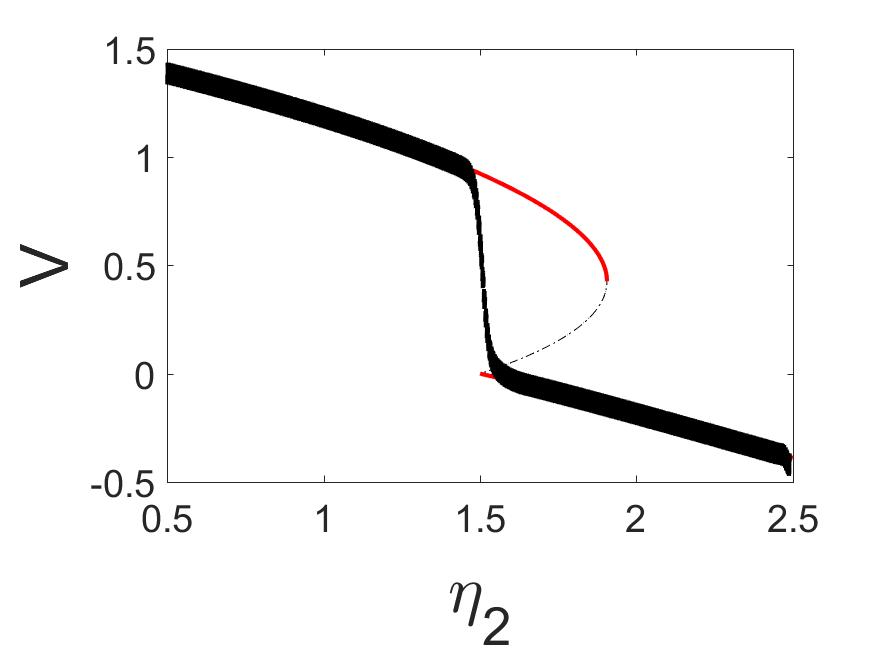
\includegraphics[width=\linewidth]{twoD/slowosc_bif_diagram_small.jpg}
  \caption{}
\end{subfigure}%
\begin{subfigure}{.5\textwidth}
  \centering
  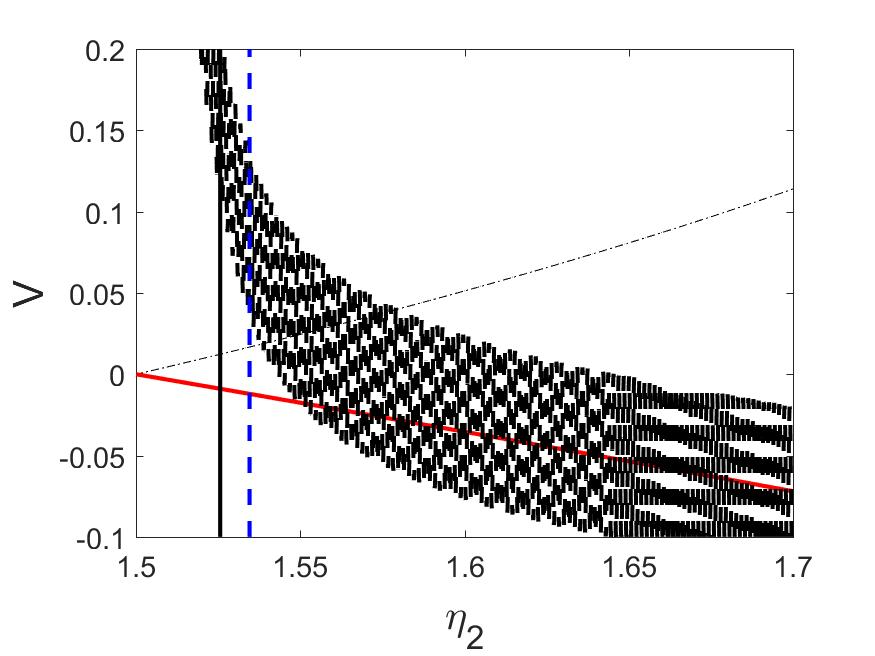
\includegraphics[width=\linewidth]{twoD/slowosc_bif_diagram_small_zoom.jpg}
  \caption{}
\end{subfigure}
\caption{Model values are $\lambda=.8$, $\epsilon=.01$ with $A=B=2$. In (a) the numerical solution (black dotted line) to \eqref{eq:twoD_canonical} is given with $\eta_1=4$, $\eta_3=.375$. In (b) a zoom in closer to the non-smooth bifurcation region where the blue dotted vertical line is the tipping point \eqref{eq:twoD_slowosc_subcaseII_tipping} and the black vertical line is the numerically obtained tipping for $V>V_{\text{smooth}}$.}
\label{fig:twoD_slowosc_Vnumerics_small}
\end{figure}

\begin{figure}[H]
\centering
\begin{subfigure}{.5\textwidth}
  \centering
  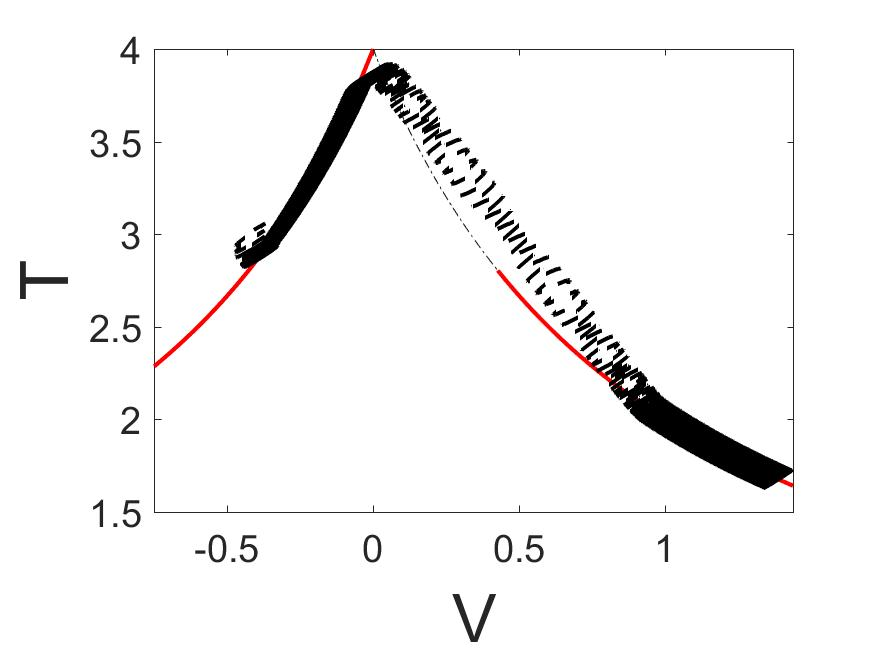
\includegraphics[width=\linewidth]{twoD/slowosc_Tplot_small.jpg}
  \caption{}
\end{subfigure}%
\begin{subfigure}{.5\textwidth}
  \centering
  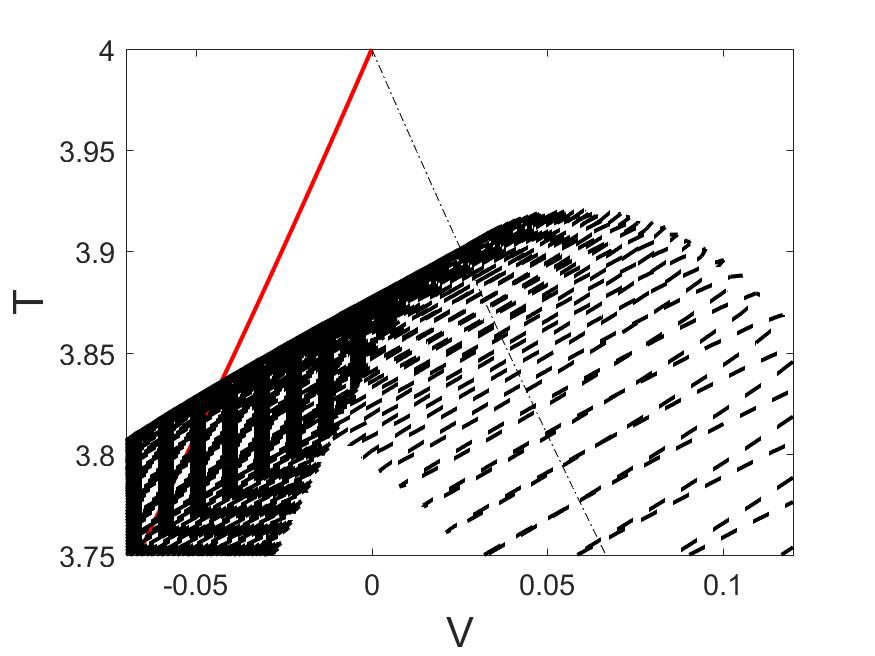
\includegraphics[width=\linewidth]{twoD/slowosc_Tplot_small_zoom.jpg}
  \caption{}
\end{subfigure}
\caption{Model values are $\lambda=.8$, $\epsilon=.01$ with $A=B=2$. In (a) we have the numerical solution (black dotted) over the static equilibrium plot for $V$ vs. $T$. In (b) a zoom of the bifurcation area.}
\label{fig:twoD_slowosc_Tnumerics_small}
\end{figure}

In figure~\ref{fig:twoD_slowosc_Vnumerics_medium} we have chosen a value of $\lambda$ in Case II as $\lambda>1$ but this choice is close to 1. Thus we see comparable behavior to Case I with the addition that the slow variation is now dominant. Upon a zoom in, it is apparent that oscillations are still present and we see the mixture of effects that cause a similar tipping to Case I to take place. We've plotted the tipping point for the slowly varying model \eqref{eq:twoD_slow_tipping} as the green vertical dotted line for comparison. As the numerical tipping point is moving towards the slowly varying tipping point this confirms that the slow variation is indeed dominating the tipping. In figure~\ref{fig:twoD_slowosc_Tnumerics_medium} we again see very similar behavior to the slowly varying model in \autoref{sec:twoD_slow} but the zoom in further reveals the oscillations are present and have minor influence by forcing the solution to cross the $V=0$ axis near the tipping.

\begin{figure}[H]
\centering
\begin{subfigure}{.5\textwidth}
  \centering
  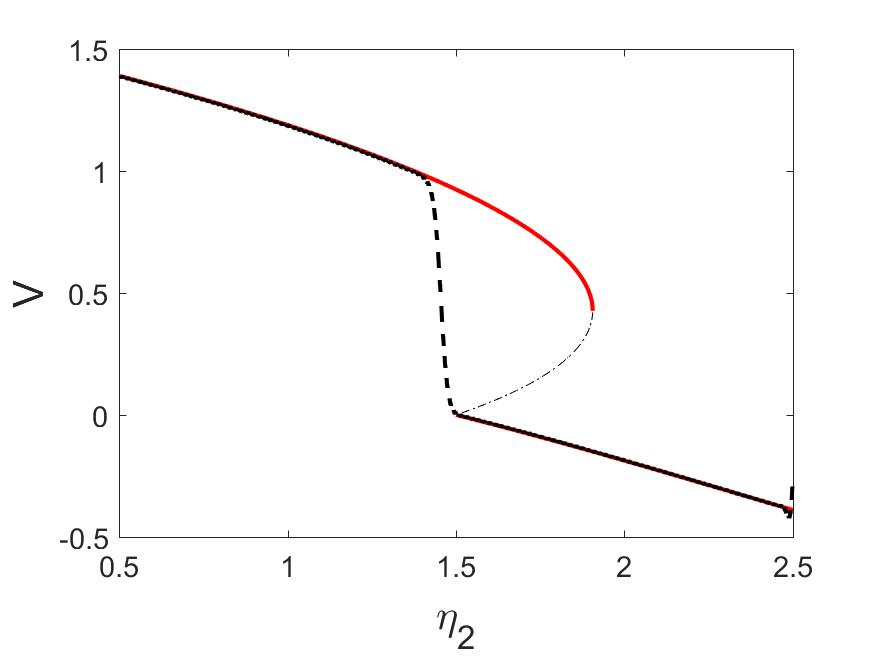
\includegraphics[width=\linewidth]{twoD/slowosc_bif_diagram_medium.jpg}
  \caption{}
\end{subfigure}%
\begin{subfigure}{.5\textwidth}
  \centering
  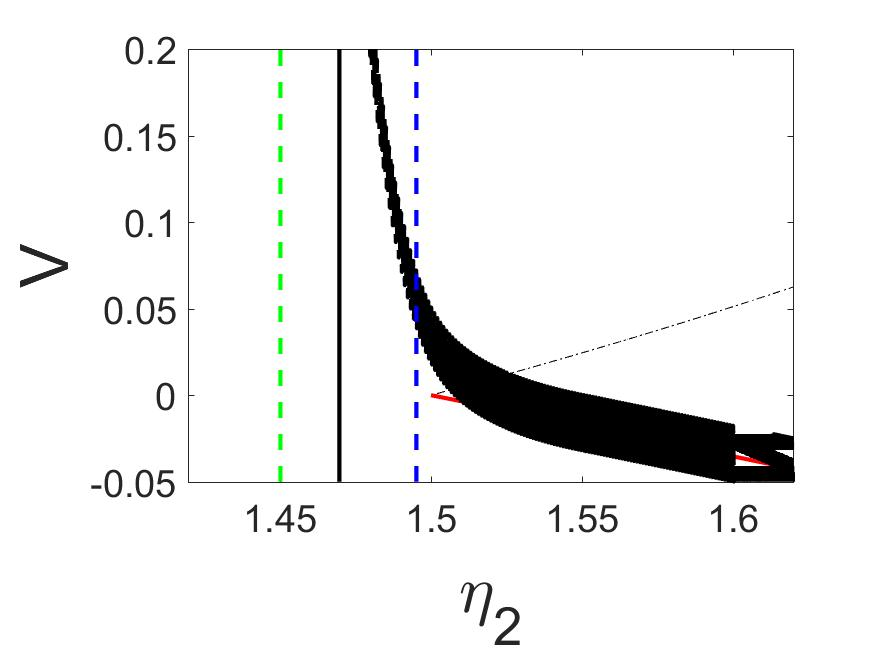
\includegraphics[width=\linewidth]{twoD/slowosc_bif_diagram_medium_zoom.jpg}
  \caption{}
\end{subfigure}
\caption{Model values are $\lambda=1.05$, $\epsilon=.01$ with $A=B=2$. In (a) the numerical solution (black dotted line) to \eqref{eq:twoD_canonical} is given with $\eta_1=4$ and $\eta_3=.375$. In (b) a zoom in closer to the non-smooth bifurcation region where the blue dotted vertical line is the mixed tipping point \eqref{eq:twoD_slowosc_subcaseII_tipping}, green dotted verticle line is the slow tipping point \eqref{eq:twoD_slow_tipping} and the black solid vertical line is the numerically obtained tipping for $V>V_{\text{smooth}}$.}
\label{fig:twoD_slowosc_Vnumerics_medium}
\end{figure}

\begin{figure}[H]
\centering
\begin{subfigure}{.5\textwidth}
  \centering
  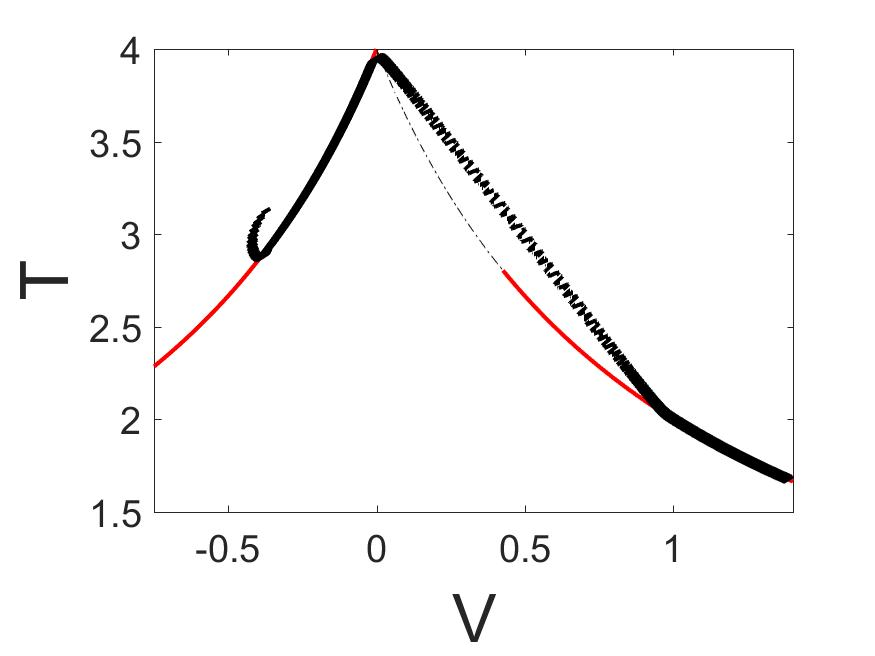
\includegraphics[width=\linewidth]{twoD/slowosc_Tplot_medium.jpg}
  \caption{}
\end{subfigure}%
\begin{subfigure}{.5\textwidth}
  \centering
  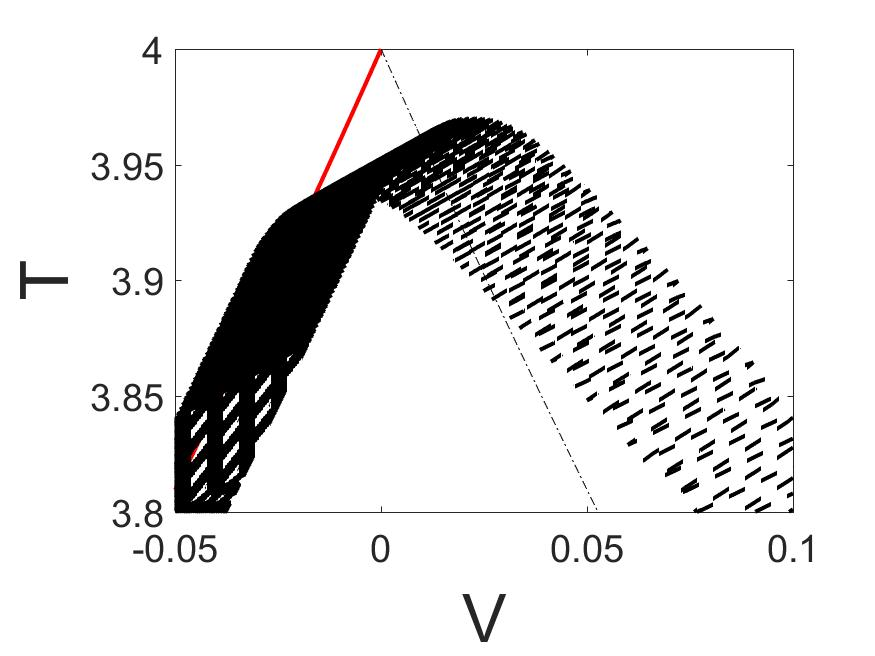
\includegraphics[width=\linewidth]{twoD/slowosc_Tplot_medium_zoom.jpg}
  \caption{}
\end{subfigure}
\caption{Model values are $\lambda=1.05$, $\epsilon=.01$ with $A=B=2$. In (a) we have the numerical solution (black dotted) over the static equilibrium plot for $V$ vs. $T$. In (b) a zoom of the bifurcation area.}
\label{fig:twoD_slowosc_Tnumerics_medium}
\end{figure}

In figure~\ref{fig:twoD_slowosc_Vnumerics_large} we show the numerics for a $\lambda$ large enough so that the oscillations are negligible and we recover the slowly varying model in \autoref{sec:twoD_slow}. Even upon a zoom it is almost impossible to see oscillations in this solution. The green dotted vertical line is the slowly varying tipping estimate \eqref{eq:twoD_slow_tipping} where the blue dotted is the mixed approximation \eqref{eq:twoD_slowosc_subcaseII_tipping}. Further evidence is seen in figure~\ref{fig:twoD_slowosc_Tnumerics_large} where this figure resembles the slowly varying $V-T$ plot \eqref{fig:twoD_slow_Tnumerics}.

\begin{figure}[H]
\centering
\begin{subfigure}{.5\textwidth}
  \centering
  \includegraphics[width=\linewidth]{twoD/slowosc_bif_diagram_large.jpg}
  \caption{}
\end{subfigure}%
\begin{subfigure}{.5\textwidth}
  \centering
  \includegraphics[width=\linewidth]{twoD/slowosc_bif_diagram_large_zoom.jpg}
  \caption{}
\end{subfigure}
\caption{ Model values are $\lambda=2$, $\epsilon=.01$ with $A=B=2$. In (a) the numerical solution (black dotted line) to \eqref{eq:twoD_canonical} is given with $\eta_1=4$ and $\eta_3=.375$. In (b) a zoom in closer to the non-smooth bifurcation region where the blue dotted vertical line is the mixed tipping point \eqref{eq:twoD_slowosc_subcaseII_tipping}, the green dotted vertical line is the slow tipping point \eqref{eq:twoD_slow_tipping} and the black vertical line is the numerically obtained tipping point for $V>V_{\text{smooth}}$.}
\label{fig:twoD_slowosc_Vnumerics_large}
\end{figure}

\begin{figure}[H]
\centering
\begin{subfigure}{.5\textwidth}
  \centering
  \includegraphics[width=\linewidth]{twoD/slowosc_Tplot_large.jpg}
  \caption{}
\end{subfigure}%
\begin{subfigure}{.5\textwidth}
  \centering
  \includegraphics[width=\linewidth]{twoD/slowosc_Tplot_large_zoom.jpg}
  \caption{}
\end{subfigure}
\caption{Model values are $\lambda=2$, $\epsilon=.01$ with $A=B=2$. In (a) we have the numerical solution (black dotted) over the static equilibrium plot for $V$ vs. $T$. In (b) a zoom of the bifurcation area.}
\label{fig:twoD_slowosc_Tnumerics_large}
\end{figure}

Although the figures above show that we have classified the behavior appropriately for the various cases in $\lambda$ and relative solution sizes, performance of our approximate tipping point needs to be evaluated to compare with numerical results. In figure~\ref{fig:twoD_slowosc_lambdacomp} we compare the tipping points between Case I and Case II with the numerically obtained tipping points across a range of $\lambda$ with a fixed $\epsilon$. For smaller $\lambda$, the frequency $\Omega$ is smaller and the influence of the oscillations on tipping become more predominant. But recall the assumption that $\Omega=\epsilon^{-\lambda}\gg 1$ and for $\lambda\le\frac{1}{2}$ we observe $\Omega\sim O(1)$. We do not consider low frequency corresponding to $\lambda<\frac{1}{2}$ in this section. For larger $\lambda$ becomes, there is a reduced influence for the oscillatory forcing until it is negligible for some $\lambda>1$. We notice that our reduction tipping approximation for $\lambda<1$ has some bias and this can be attributed the information lost from reducing the full two-dimensional Riccati equations to a one-dimensional model. Although we use a one-dimensional reduced equation to get these approximations, they seem to be performing quite well across all $\lambda$ hence validating the method developed for tipping with varying $\lambda$.

\begin{figure}[H]
\centering
\includegraphics[width=0.7\textwidth]{twoD/slowosc_lambdacomp.jpg}
\caption{An example of numerical tipping (red stars) as the numerical solution to \eqref{eq:oneD_canonical} passes $V>V_{\text{smooth}}$. Parameter values are $\epsilon=.01$ and $A=B=3$. The lines are the Case I tipping estimate (black solid line) and the Case II tipping estimate (blue dotted line).}
\label{fig:twoD_slowosc_lambdacomp}
\end{figure} 

We also are interested in the performance of the tipping approximations across values of $\epsilon$ for $\lambda$ fixed. The performance of each estimate is seen in figure~\ref{fig:twoD_slowosc_epscomp}. For Case I tipping, the range of appropriate $\epsilon$ is highly dependent on the choice in $\lambda$. Often, the range is very small to get accurate estimates. Once this range is left, there are interesting phase effects for the tipping which causes oscillations in the numeric tipping points. For Case II tipping, we that there is a transition happening towards the purely slow tipping, similarly to \autoref{sec:twoD_slow}


\begin{figure}[H]
\centering
\begin{subfigure}{.5\textwidth}
  \centering
  \includegraphics[width=\linewidth]{twoD/slowosc_epscomp_mixed.jpg}
  \caption{$\lambda=.8$}
\end{subfigure}%
\begin{subfigure}{.5\textwidth}
  \centering
  \includegraphics[width=\linewidth]{twoD/slowosc_epscomp_slow.jpg}
  \caption{$\lambda=1.3$}
\end{subfigure}
\caption{The numerical tipping (red stars) follows the appropriate case depending on $\lambda$ for $\epsilon=0.01$. The Case I tipping estimate (black solid line) and purely slow tipping estimate (blue dotted line) are shown.}
\label{fig:twoD_slowosc_epscomp}
\end{figure}

With the numerical results agreeing with our results, we may finally conclude that this method is both useful for analyzing the non-smooth behavior in the Stommel model but also results in an approximation that is more accurate in the extremes of the model (i.e $\Omega \gg 1$ or $\epsilon \ll 1$). This gives us a very accessible means of extracting the tipping in the full two-dimensional without needing to solve difficult Riccati equations or other complex systems that appear from the full problem. All that is needed to verify is our solutions remain stable until we arrive at the region of tipping.

\subsection{Stability}

\subsubsection{Case I: $\lambda\le 1$}

From the analysis, we had discovered the inner equations that govern the behavior of the solution for this range of $\lambda$ are

\begin{equation}\label{eq:twoD_slowosc_stability_caseI_full}
\begin{aligned}
{P_0}_t =& -\epsilon^{1-\lambda} n(t)-\eta_2 P_0 -(1-\eta_3)Q_0,\\
{Q_0}_t =& -\frac{\eta_1}{2\pi}\int_0^{2\pi}|P_0-A\cos(R)|\,dR - Q_0.
\end{aligned}
\end{equation}

But we also found that the relative size of $P_0(t)$ dictates the difficulty of \eqref{eq:twoD_slowosc_stability_caseI_full}. In the analysis we treat these as Sub-Case I: $P_0(t)\le-|A|$ and Sub-Case II: $|P_0(t)|<|A|$ which each require a separate analysis due to their differing behavior.

\subsubsection{Sub-Case I: $P_0(t)\le-|A|$}

We called this the entirely below-axis sub-case due to the solution remaining below the axis and hence predictable under these conditions thus we anticipate this sub-case to remain stable. The equation \eqref{eq:twoD_slowosc_stability_caseI_full} simplifies for this sub-case to

\begin{equation}\label{eq:twoD_slowosc_stability_subcaseI_full}
\begin{aligned}
{P_0}_t =& -\epsilon^{1-\lambda} n(t)-\eta_2 P_0 -(1-\eta_3)Q_0,\\
{Q_0}_t =& \eta_1 P_0 - Q_0.
\end{aligned}
\end{equation}

Which from the analysis we choose to reduce \eqref{eq:twoD_slowosc_stability_subcaseI_full} with the pseudo-equilibria $Q_0(P_0)=\eta_1 P_0$. This gives the following one-dimensional equation with it's pseudo-equilibria as 

\begin{equation}\label{eq:twoD_slowosc_stability_subcaseI_reduced}
\begin{aligned}
{P_0}_t =& -\epsilon^{1-\lambda}n(t)-(\eta_3+\eta_1(1-\eta_3))P_0=f(t,P_0),\\ Z^0(t) =& -\epsilon^{1-\lambda}\frac{n(t)}{\eta_3+\eta_1(1-\eta_3)}.
\end{aligned}
\end{equation}

We adopt a similar strategy for analyzing the stability from the one-dimensional model in \autoref{sec:oneD_slowosc} due to \eqref{eq:twoD_slowosc_stability_subcaseI_reduced} being a one-dimensional equation. Hence we take a simple linear perturbation about the pseudo-equilibrium with $P_0(t)=Z^0(t)+U(t)$ and $\lVert U(t)\rVert \ll 1$. Taking special care to note that $Z^0(t)$ also varies in time, we find the Taylor approximation

\begin{equation}\label{eq:twoD_slowosc_subcaseI_perturb}
\begin{aligned}
{P_0}_t=&f(t,Z^0) +f_{P_0}(t,Z^0)(P_0(t)-Z^0(t))+O(\lVert (P_0(t)-Z^0(t))^2\rVert^2),\\
U_t+Z^0_t =& -(\eta_3+\eta_1(1-\eta_3))U,\\
U_t =& -\epsilon^{1-\lambda}\frac{1}{\eta_3+\eta_1(1-\eta_3)}-(\eta_3+\eta_1(1-\eta_3))U.
\end{aligned}
\end{equation}

With \eqref{eq:twoD_slowosc_subcaseI_perturb} we find that the perturbations decay exponentially to a nearby equilibrium. This indicates the solution for this sub-case is hyperbolically stable and further agrees that no tipping will happen for this size of the solution.

\subsubsection{Sub-Case II: $|P_0(t)|<-|A|$}

We called this the crossing case and from the analysis we anticipate the tipping to occur as the solution is gradually becoming uncontrollable with the crossing. Under the conditions of this sub-case, we integrate \eqref{eq:twoD_slowosc_stability_caseI_full} with the $R_1$ and $R_2$ from the analysis and take the same Taylor approximation to find 

\begin{equation}\label{eq:twoD_slowosc_stability_subcaseII,full}
\begin{aligned}
{P_0}_t =& -n(t)-\eta_3 P_0-(1-\eta_3)Q_0,\\
{Q_0}_t =&-\epsilon^{\lambda-1}\frac{2\eta_1|A|}{\pi}-\epsilon^{1-\lambda}\frac{\eta_1(1-\eta_3)}{\pi|A|}P_0^2-Q_0.
\end{aligned}
\end{equation}

Once more, we assume that the equation for $Q_0$ is in pseudo-equilibrium 
to reduce to the following one-dimensional inner equation with equilibrium where here we let $a=\frac{\eta_1(1-\eta_3)}{\pi|A|}$ for simplicity

\begin{equation}\label{eq:twoD_slowosc_stability_subcaseII,reduced}
\begin{aligned}
{P_0}_t =& -\epsilon^{1-\lambda}n(t)+\frac{2\eta_1(1-\eta_3)|A|}{\pi}-\eta_3 P_0+aP_0^2=f(t,P_0),\\
Z^0(t) =& \frac{1}{2a}\left(\eta_3-\sqrt{4a(\epsilon^{1-\lambda}n(t)-n_{\text{osc}})}\right).
\end{aligned}
\end{equation}

Where we choose to write the argument of the square root in terms of the bifurcation found in \eqref{eq:twoD_osc_bifurcation}. We then consider the linear perturbation about the pseudo-equilibrium $P_0(t)= Z^0(t)+U(t)$ with $\lVert U\rVert \ll 1$. We take a Taylor expansion here to find the dynamics of the perturbation, but recall that we have contributions to the derivative from both the perturbation as well as the pseudo-equilibrium. This is seen with

\begin{equation}
\begin{aligned}
{P_0}_t =& Z^0_t+U_t,\\
Z^0_t=&\begin{cases}
\frac{\epsilon^{1-\lambda}}{\sqrt{4a(\epsilon^{1-\lambda}n(t)-n_{\text{osc}})}} & \epsilon^{1-\lambda}n(t)>n_{\text{osc}},\\
0 & \epsilon^{1-\lambda}n(t)=n_{\text{osc}}.
\end{cases}
\end{aligned}
\end{equation}

Thus we find the following Taylor expansion for the perturbations

\begin{equation}\label{eq:twoD_slowosc_stability_subcaseII_perturb}
\begin{aligned}
{P_0}_t =& f(t,Z^0)+f_{P_0}(t,Z^0)(P_0-Z^0)+O(\lVert P_0-Z^0 \rVert^2),\\
U_t+Z^0_t=& -\sqrt{4a(\epsilon^{1-\lambda}n(t)-n_{\text{osc}})} U,\\
 U_t = & \begin{cases}
\frac{\epsilon^{1-\lambda}}{\sqrt{4a(\epsilon^{1-\lambda}n(t)-n_{\text{osc}})}}-\left(\sqrt{4a(\epsilon^{1-\lambda}n(t)-n_{\text{osc}})}\right) U & \epsilon^{1-\lambda}n(t)>n_{\text{osc}},\\
0 & \epsilon^{1-\lambda}n(t)=n_{\text{osc}}.
\end{cases}
\end{aligned}
\end{equation}

From \eqref{eq:twoD_slowosc_stability_subcaseII_perturb} we find exponentially decaying perturbations that give asymptotic stability until we get to the oscillatory bifurcation. The oscillatory bifurcation corresponds to non-hyperbolic behavior and we lose stability shortly after which indicates of the tipping to occur after the bifurcation.

\subsubsection{Case II: $\lambda>1$}

From the analysis we determined this to be the slowly dominant case and we had discovered the inner equations that govern the behavior of the solution for this range of $\lambda$ to be

\begin{equation}\label{eq:twoD_slowosc_caseII_full}
\begin{aligned}
{P_0}_t =& - n(t)-\eta_2 P_0 -(1-\eta_3)Q_0,\\
{Q_0}_t =& -\frac{\eta_1}{2\pi}\int_0^{2\pi}|P_0-\epsilon^{\lambda-1} A\cos(R)|\,dR - Q_0.
\end{aligned}
\end{equation}

The behavior of this case when $\lambda\sim 1$ is very similar to Case I, thus we anticipate the stability to behave similarly as well. Hence we consider the behavior when $|P_0(t)|<\epsilon^{\lambda-1}|A|$ which is where we found tipping to occur in the analysis. As long as we have $\epsilon^{\lambda-1}A\sim O(1)$, we are follow the same approach as Case I where we integrate \eqref{eq:twoD_slowosc_caseII_full} with a similar $R_1$ and $R_2$ and use a Taylor approximation to get

\begin{equation*}
\begin{aligned}
{P_0}_t =& - n(t)-\eta_2 P_0 -(1-\eta_3)Q_0,\\
{Q_0}_t =& -\epsilon^{\lambda-1}\frac{2\eta_1(1-\eta_3)|A|}{\pi}-\epsilon^{1-\lambda}\frac{\eta_1}{\pi|A|}P_0^2- Q_0.
\end{aligned}
\end{equation*}

The analysis gave sufficient reason to reduce the inner equations to a one-dimensional model and thus like in Case I w find the inner equation with pseudo-equilibrium where here we let $a=\frac{\eta_1(1-\eta_3)}{\pi|A|}$ for simplicity

\begin{equation*}
\begin{aligned}
{P_0}_t =& -n(t)+\epsilon^{\lambda-1}\frac{2\eta_1(1-\eta_3)|A|}{\pi}-\eta_3 P_0+\epsilon^{1-\lambda}aP_0^2,\\
Z^0(t) =& \frac{1}{2a}\left(\epsilon^{\lambda-1}\eta_3-\sqrt{\epsilon^{\lambda-1}4a(n(t)-\epsilon^{\lambda-1}n_{\text{osc}})}\right)
\end{aligned}
\end{equation*}

Where we consider the linear perturbation about the pseudo-equilibrium $P_0(t)= Z^0(t)_U(t)$ with $\lVert U\rVert \ll 1$. We take a Taylor expansion here to find the dynamics of the perturbation, but recall that we have contributions to the derivative from both the perturbation as well as the pseudo-equilibrium. This is seen with

\begin{equation}
\begin{aligned}
{P_0}_t =& Z^0_t+U_t,\\
Z^0_t=&\begin{cases}
\frac{\epsilon^{(\lambda-1)/2}}{\sqrt{4a(n(t)-\epsilon^{\lambda-1}n_{\text{osc}})}} & n(t)>\epsilon^{\lambda-1}n_{\text{osc}},\\
0 & n(t)=\epsilon^{\lambda-1}n_{\text{osc}}.
\end{cases}
\end{aligned}
\end{equation}

Thus we find the following Taylor expansion for the perturbations

\begin{equation}\label{eq:twoD_slowosc_stability_caseII_perturb}
\begin{aligned}
{P_0}_t =& f(t,Z^0)+f_{P_0}(t,Z^0)(P_0-Z^0)+O(\lVert P_0-Z^0 \rVert^2),\\
U_t+Z^0_t=& -\left(\sqrt{\epsilon^{1-\lambda}4a(n(t)-\epsilon^{\lambda-1}n_{\text{osc}})}\right) U,\\
U_t = & \begin{cases}
\frac{\epsilon^{(\lambda-1)/2}}{\sqrt{4a(n(t)-\epsilon^{\lambda-1}n_{\text{osc}})}}-\left(\sqrt{\epsilon^{1-\lambda}4a(n(t)-n_{\text{osc}})}\right) U & n(t)>\epsilon^{\lambda-1}n_{\text{osc}},\\
0 & n(t)=\epsilon^{\lambda-1}n_{\text{osc}}.
\end{cases}
\end{aligned}
\end{equation}

From \eqref{eq:twoD_slowosc_stability_caseII_perturb} we find that the perturbations decay exponentially and we have asymptotic stability until we get to the oscillatory bifurcation. The bifurcation found in \eqref{eq:twoD_osc_bifurcation} corresponds to non-hyperbolic behavior and we then lose the stability which indicates of the tipping to occur after the bifurcation. Comparing this to Case I, we see there is small nuances between these perturbations, although the overall stability remains the same. As for when $\lambda$ grows, we already established this behaves like the purely slow model and hence we can use the stability from that section to conclude that our solution is still stable until the slow tipping point, at which we lose stability as anticipated.


Thus the stability for both Case I and Case II agrees with the results found in the analysis. We have that the behavior of the solution is stable from the outer solution, stability holds before the solution begins to cross the axis $V=0$ and once the crossing begins to happen we lose stability at the location of the oscillatory bifurcation. Because there is slow variation in this model, there is still delayed behavior and thus the tipping happens shorty after the oscillatory bifurcation. In both cases we discovered that the pseudo-equilibrium has a contribution to the derivative and this in turn causes the perturbations to decay towards a small constant. This means that there is a small region around the pseudo-equilibrium that attracts the solution and this is seen in the numerical results. 


\chapter{Summary and Future Work}
\label{chap:conclusion}
With the results found in this paper, we have accurately described what kind of behavior is present about the non-smooth bifurcation when new mechanisms are introduced in both the one-dimensional model \eqref{eq:oneD_canonical} and two-dimensional Stommel model \eqref{eq:twoD_canonical}. We had considered the mixture of early bifurcation due to high oscillatory forcing $\Omega\gg 1$ with amplitude $A\sim O(1)$ and the delayed tipping due to slow variation in the bifurcating parameter at rate $\epsilon\ll 1$. The main result being that these mechanisms have opposite effects on the tipping point and do mix with a kind of weighted average to produce an effective tipping approximation. These results give insight into the hysteresis behavior of the Stommel model and the understudied realm of non-smooth dynamics. The main approach used asymptotic expansions as well as the methods of multiple scales to identify reduced equations and find asymptotic solutions to the systems of differential equations. We found that depending on the region and mechanism, the reduced equations have differing expressions depending on the size of the solution. We also discover that linking the slow variation $\epsilon$ and the frequency $\Omega$ gives important insight into how the system will behave. 

The method developed in the one-dimensional model was to find an outer asymptotic expansion by separating the order of dynamics by a common small value, typically in terms of $\epsilon$. With the outer dynamics explicitly written, we scaled the model to find the inner equations to a reduced problem. From the inner equations, we solve and determine when the solution is no longer controllable. This resulted in the tipping points/bifurcations in the one-dimensional system \eqref{eq:oneD_canonical} which had good agreement with the numerical results from a simple differential equation solver. Due to the many similarities to the two-dimensional system \eqref{eq:twoD_canonical} we were able to modify the same analysis to find the tipping/bifurcations here as well.

Although the work here is not entirely finished where an analysis would need to be done on cases where $\Omega\sim O(1)$ or smaller. This case functions qualitatively different as slow oscillations have more contribution to the dynamics. This is also seen from the analysis where low frequency oscillations no longer allow for asymptotic expansions in terms of $\Omega^{-1}$ and no longer fall under our assumptions to integrate with $T_1$ and $T_2$. Thus this case behaves fundamentally different and can influence tipping in a way we hadn't explored here. This is shown in figure~\ref{fig:low_freq}. Also, large amplitude behavior $A\gg 1$ can force an additional rescaling before any familiar approaches hold. This is seen in figure~\ref{fig:large_amp}. These cases were mentioned but have yet to be performed on this model, although both have been studied around the smooth case in \cite{zhu2015tipping}. It is possible that they could have some surprising results in the non-smooth case. These cases would help further classify the tipping behavior for the variety of cases in real world ocean dynamics.

\begin{figure}[H]
\centering
\begin{subfigure}{.5\textwidth}
 \centering
 \includegraphics[width=\linewidth]{conclusion/low_freq_V.jpg}
 \caption{}
\end{subfigure}%
\begin{subfigure}{.5\textwidth}
 \centering
 \includegraphics[width=\linewidth]{conclusion/low_freq_T.jpg}
 \caption{}
\end{subfigure}
\caption{Low Frequency: Model parameters are $\epsilon=.01$, $A=B=1$ and $\Omega=3$.}
\label{fig:low_freq}
\end{figure}

\begin{figure}[H]
\centering
\begin{subfigure}{.5\textwidth}
 \centering
 \includegraphics[width=\linewidth]{conclusion/large_amp_V.jpg}
 \caption{}
\end{subfigure}%
\begin{subfigure}{.5\textwidth}
 \centering
 \includegraphics[width=\linewidth]{conclusion/large_amp_T.jpg}
 \caption{}
\end{subfigure}
\caption{Large Amplitude: Model parameters are $\epsilon=.01$, $A=B=300$ and $\Omega=1000$.}
\label{fig:large_amp}
\end{figure}

Lastly, we considered all deterministic behavior throughout this analysis but there are many reasons to incorporate stochastic elements into the Stommel model as well, see \cite{lorenzo2012role}. From \cite{zhu2015tipping} it is concluded that stochastic forcing has elements of both early bifurcations and delayed tipping and thus a natural follow-up to the analysis in this paper. We could consider stochastic forcing with

\begin{equation}\label{eq:stochastic}
\begin{aligned}
\dot{V} & = \eta_1-\eta_2+\eta_3(T-V)-T-V|V|+A\xi_1(t), \\
  \dot{T}   & = \eta_1-T(1+|V|)+B\xi_2(t), \\
 \dot{\eta_2} & = -\epsilon\\
 V(0)=&V^0,\quad T(0)=T^0, \quad \eta_2(0)={\eta_2}^0,
\end{aligned}
\end{equation}

where $\xi_i(t)$ is standard Gaussian noise with mean 0 and variance $t$ and initial conditions centered on the lower branch. This is shown in figure~\ref{fig:stochastic} and it is clear a completely separate analysis is needed.

\begin{figure}[H]
\centering
\begin{subfigure}{.5\textwidth}
 \centering
 \includegraphics[width=\linewidth]{conclusion/stochastic_V.jpg}
 \caption{}
\end{subfigure}%
\begin{subfigure}{.5\textwidth}
 \centering
 \includegraphics[width=\linewidth]{conclusion/stochastic_V_zoom.jpg}
 \caption{}
\end{subfigure}
\begin{subfigure}{.5\textwidth}
 \centering
 \includegraphics[width=\linewidth]{conclusion/stochastic_T.jpg}
 \caption{}
\end{subfigure}%
\begin{subfigure}{.5\textwidth}
 \centering
 \includegraphics[width=\linewidth]{conclusion/stochastic_T_zoom.jpg}
 \caption{}
\end{subfigure}
\caption{Stochastic: In (a) many realizations of the numerical solution for $V$ in \eqref{eq:stochastic} is given with model parameters $\eta_1=4$, $\eta_3=.375$, $\epsilon=.01$ and $A=B=.7$. In (b) a zoom in closer to the non-smooth bifurcation region. In (c) we have the realizations over the standard equilibrium plot for $V$ vs. $T$. In (d) a zoom of the bifurcation area.}
\label{fig:stochastic}
\end{figure}

%%% Note: the bibliography must come before the appendices.
\bibliographystyle{plain}
\bibliography{thesis_bib}

%% Use this to reset the appendix counter.  Note that the FoGS
%% requires that the word ``Appendices'' appear in the table of
%% contents either before each appendix lable or as a division
%% denoting the start of the appendices.  We take the latter option
%% here.  This is ensured by making the \texttt{appendicestoc} option
%% a default option to the UBC thesis class.

%%% If you only have one appendix, please uncomment the following line.
% \renewcommand{\appendicesname}{Appendix}
\appendix
\chapter{The Stommel Model}
\label{app:stommel}
\input{chapters/stommelappendix.tex}

\chapter{One Component}
\label{app:oneD}
\section*{High Frequency Oscillatory Forcing}

Here we continue the analysis to explicitly find the solution of the outer equation for the purely oscillatory model. Recall that we found $x_1 = v_1(t)-A\cos(T)$, we then apply the Fredholm alternative \eqref{eq:Fredholm} to the $O(\Omega^{-2})$ equation in \eqref{eq:oneD_osc_outerO3} to get

\begin{equation}\label{eq:oneD_app_osc}
\begin{aligned}
0=&\frac{1}{2\pi}\int_0^{2\pi}-{x_1}_t-2x_1+2x_0x_1\, dT,\\
{v_1}_t=& -2v_1+2(1-\sqrt{1+\mu})v_1,\\
{v_1}_t=& -2\sqrt{1+\mu}v_1.
\end{aligned}
\end{equation}

We search for the equilibrium to find stable behavior on this order but since \eqref{eq:oneD_app_osc} has a very simple form, the equilibrium is $v_1(t)\equiv 0$ and thus we find the correction term to only have oscillatory behavior, $x_1=-A\cos(T)$.

\section*{Slow Variation and Oscillatory Forcing}

Here we continue to find the terms of the outer solution for the slowly varying and oscillatory forcing model. We have thus far found $x_0=x_0(\tau)$ and we have equations at $O(\epsilon^\lambda)$ and $O(\epsilon^{2\lambda})$ that give information about $x_0$ and $x_1$ respectively. We apply the Fredholm alternative \eqref{eq:Fredholm} to the $O(\epsilon^\lambda)$ equation \eqref{eq:oneD_slowosc_outerO2} to find

\begin{equation}\label{eq:oneD_app_slowosc1}
\begin{aligned}
0 = & \frac{1}{2\pi}\int_0^{2\pi} -\mu(\tau) -2x_0(\tau)+x_0(\tau)^2+A\sin(T)\,dT,\\
0=&-\mu(\tau)-2x_0(\tau)+x_0(\tau)^2,\\
x_0(\tau) =& 1-\sqrt{1+\mu(\tau)},\\
{x_1}_T = & A\sin(T).
\end{aligned}
\end{equation}

From \eqref{eq:oneD_app_slowosc1} we find that $x_1=v_1(\tau)-A\cos(T)$, which gives us access to solving the next order equation. Thus we now do the same for the $O(\epsilon^{2\lambda})$ equation \eqref{eq:oneD_slowosc_outerO3} to find

\begin{equation}
\begin{aligned}
0=&\frac{1}{2\pi}\int_0^{2\pi}-\epsilon^{1-\lambda}{x_0}_\tau -2x_1+2x_0x_1\,dT,\\
\epsilon^{1-\lambda}{x_0}_\tau=& -2v_1+2(1-\sqrt{1+\mu(\tau)})v_1,\\
v_1(\tau) =& -\epsilon^{1-\lambda}\frac{{x_0}_\tau}{2\sqrt{1+\mu(\tau)}}.
\end{aligned}
\end{equation}

Recall that $\mu_\tau=-1$ and that ${x_0}_\tau = -\frac{{\mu}_\tau}{2\sqrt{1+\mu(\tau)}}=\frac{1}{2\sqrt{1+\mu(\tau)}}$ and thus we find the form of the next order term in the expansion as

\begin{equation}
x_1(\tau,T) = -\epsilon^{1-\lambda}\frac{1}{4(1+\mu(\tau))}-A\cos(T).
\end{equation}

\chapter{Two Component}
\label{app:twoD}
\section*{High Frequency Oscillatory Forcing}

Here we show that the correction term of the outer solution is purely oscillatory. From the analysis, we found both leading order terms to be purely slow time dependent, i.e. $V_0=V_0(\tau)$ and $T_0=T_0(\tau)$. To find the explicit form for these, we apply Fredholm \eqref{eq:Fredholm} to the $O(\Omega^{-1})$ equations in \eqref{eq:twoD_osc_outerO2} to find

\begin{equation}\label{eq:twoD_app_osc1}
\begin{aligned}
&\begin{cases}
	0 = & \frac{1}{2\pi}\int_0^{2\pi}-{V_0}_t+\eta_1-\eta_2+\eta_3(T_0-V_0)-T_0+V_0^2+A\sin(R)\,dR,\\
	 0 =& \frac{1}{2\pi}\int_0^{2\pi}-{T_0}_t+ \eta_1-T_0(1-V_0)+B\sin(R)\,dR,
\end{cases}\\
&\begin{cases}
	{V_0}_t = & \eta_1-\eta_2+\eta_3(T_0-V_0)-T_0+V_0^2,\\
	 {T_0}_t =&  \eta_1-T_0(1-V_0),
\end{cases}\\
& {V_1}_R = A\sin(R),\quad {T_1}_R = B\cos(R).
\end{aligned}
\end{equation}

Since we have a fixed parameter $\eta_2$, we find the equilibria $V_0$ and $T_0$ as well as the form of the correction terms

\begin{equation*}
\begin{aligned}
T_0&(V_0) = \frac{\eta_1}{1-V_0},\\
0= & \eta_1-\eta_2 +\eta_3(T_0(V_0)-V_0)-T_0(V_0)+V_0^2,\\
V_1 =& X_1(t)-A\cos(R),  \quad T_1 = Y_1(t)-B\cos(R).
\end{aligned}
\end{equation*}

Here we note these equilibria to be the same as in the static problem with no forcing from the introduction. But with the form of the correction terms, we now solve the equation at $O(\Omega^{-2})$ \eqref{eq:twoD_osc_outerO3} by applying Fredholm \eqref{eq:Fredholm}. This results in

\begin{equation}\label{eq:twoD_app_osc2}
\begin{aligned}
&\begin{cases}
	0 = & \frac{1}{2\pi}\int_0^{2\pi}-{V_1}_t+\eta_3(T_1-V_1)-T_1+2V_0V_1\,dR,\\
	 0 =& \frac{1}{2\pi}\int_0^{2\pi}-{T_1}_t+ T_1(1-V_0)+T_0V_1\,dR,
\end{cases}\\
&\begin{cases}
	{X_1}_t = & \eta_3(Y_1-X_1)-Y_1+2X_0X_1,\\
	 {Y_1}_t =&  Y_1(1-X_0)+Y_0X_1.
\end{cases}
\end{aligned}
\end{equation}

We then search for the equilibria of \eqref{eq:twoD_app_osc2} and find

\begin{equation*}
\begin{aligned}
Y_1&(X_1) =-\frac{Y_0X_1}{1-X_0},\\
0 =& \left(\eta_3\left(\frac{Y_0}{1-X_0}-1\right)-\frac{Y_0}{1-X_0}+2X_0\right)X_1.
\end{aligned}
\end{equation*}

Thus we find that the correction terms are purely oscillatory since $X_1\equiv 0$ and $Y_1 \equiv 0$. This gives $V_1=-A\cos(R)$ and $T_1=-B\cos(R)$.

\section*{Slow Variation and Oscillatory Forcing}

Here we continue to find terms of the outer solution by working through the equations \eqref{eq:twoD_slowosc_outerO2}-\eqref{eq:twoD_slowosc_outerO3}. In the analysis, we had already determined that the leading order terms are purely slow time dependent, $V_0=V_0(\tau)$ and $T_0=T_0(\tau)$. To find their exact form, we apply Fredholm \eqref{eq:Fredholm} to the $O(\epsilon^\lambda)$ equation \eqref{eq:twoD_slowosc_outerO2} to find 

\begin{equation}\label{eq:twoD_app_slowosc1}
\begin{aligned}
&\begin{cases}
	0 = & \frac{1}{2\pi}\int_0^{2\pi}\eta_1-\eta_2(\tau)+\eta_3(T_0-V_0)-T_0+V_0^2+A\sin(R)\,dR,\\
	 0 =& \frac{1}{2\pi}\int_0^{2\pi} \eta_1-T_0(1-V_0)+B\sin(R)\,dR,
\end{cases}\\
&\begin{cases}
	0 = & \eta_1-\eta_2(\tau)+\eta_3(T_0-V_0)-T_0+V_0^2,\\
	 0 =&  \eta_1-T_0(1-V_0),
\end{cases}\\
& {V_1}_R = A\sin(R),\quad {T_1}_R = B\cos(R).
\end{aligned}
\end{equation}

The leading order solution to \eqref{eq:twoD_app_slowosc1} is the same as the slowly varying problem from \autoref{sec:twoD_slow} with

\begin{equation*}
\begin{aligned}
T_0&(V_0)=\frac{\eta_3}{1-V_0},\\
0=& \eta_1-\eta_2(\tau)+\eta_3(T_0(V_0)-V_0)-T_0(V_0)+V_0^2.
\end{aligned}
\end{equation*}

We also find the form of the correction terms, $V_1 = X_1(\tau) -A\cos(R)$ and $T_1 = Y_1(\tau)-B\cos(R)$, which allow us to solve the $O(\epsilon^{2\lambda})$ equation \eqref{eq:twoD_slowosc_outerO3}. Applying Fredholm \eqref{eq:Fredholm} here results in 

\begin{equation}\label{eq:twoD_app_slowosc2}
\begin{aligned}
&\begin{cases}
	0 = & \frac{1}{2\pi}\int_0^{2\pi}\left(-\epsilon^{1-\lambda}{V_0}_\tau+\eta_3(T_1-V_1)-T_1+2V_0V_1+A\sin(R)\right)\,dR,\\
	 0 =& \frac{1}{2\pi}\int_0^{2\pi} \left(\epsilon^{1-\lambda}{T_0}_\tau-T_1(1-V_0)+T_0V_1\right)\,dR,
\end{cases}\\
&\begin{cases}
	\epsilon^{1-\lambda}{V_0}_\tau=&\eta_3(Y_1-X_1)-Y_1+2V_0X_1, \\
	 \epsilon^{1-\lambda}{T_0}_\tau =&  Y_1(1-V_0)+T_0X_1.
\end{cases}
\end{aligned}
\end{equation}

Recalling that ${\eta_2}_\tau=-1$ and solving \eqref{eq:twoD_app_slowosc2} requires the derivatives of $V_0$ and $T_0$ which are solvable explicitly as

\begin{equation*}
\begin{aligned}
{T_0}_\tau&({V_0}_\tau) = -\frac{\eta_1{V_0}_\tau}{1-V_0},\\
{V_0}_\tau &=\frac{(1-V_0)}{\eta_1+\eta_3(\eta_1+1-V_0)-2V_0(1-V_0)}. 
\end{aligned}
\end{equation*}

With everything put together, we find the solution to \eqref{eq:twoD_app_slowosc2} as 

\begin{equation*}
\begin{aligned}
Y_1(X_1) =& \frac{\epsilon^{1-\lambda}{T_0}_\tau-T_0X_1}{1-V_0},\\
X_1=&\frac{\epsilon^{1-\lambda}({V_0}_\tau(1-V_0)+(1-\eta_3){T_0}_\tau)}{(1-\eta_3)T_0+(2V_0-\eta_3)(1-V_0)}.
\end{aligned}
\end{equation*}

Here we now have the first correction term as

\begin{equation*}
\begin{aligned}
V_1(\tau,R)=& \frac{\epsilon^{1-\lambda}({V_0}_\tau(1-V_0)+(1-\eta_3){T_0}_\tau)}{(1-\eta_3)T_0+((2V_0-\eta_3)(1-V_0)}-A\cos(R),\\
T_1(\tau,R)=&\frac{\epsilon^{1-\lambda}{T_0}_\tau}{1-V_0}-\frac{\epsilon^{1-\lambda}T_0({V_0}_\tau(1-V_0)+(1-\eta_3){T_0}_\tau)}{(1-\eta_3)T_0(1-V_0)+(2V_0-\eta_3)(1-V_0)^2}-B\cos(R).
\end{aligned}
\end{equation*}

\backmatter

\end{document}
\endinput
%%
%% End of file `ubcsample.tex'.
